%-----------------------------------------------------------------
% Modelo de Tese/Dissertação
% Autora: Fabiana Frata Furlan Peres 
% 2014 
%-----------------------------------------------------------------
%% ADAPTADO DE:
%% modelo de Documento TCC da Unioeste   
%%
%% que por sua vez foi ADAPTADO DE: 
%% abtex2-modelo-trabalho-academico.tex, v-1.6 laurocesar
%% Copyright 2012-2013 by abnTeX2 group at http://abntex2.googlecode.com/ 
% ------------------------------------------------------------------------
% abnTeX2: Modelo de Trabalho Academico (tese de doutorado, dissertacao de
% mestrado e trabalhos monograficos em geral) em conformidade com 
% ABNT NBR 14724:2011: Informacao e documentacao - Trabalhos academicos - Apresentacao
%
% ------------------------------------------------------------------------
%DECLARAÇÃO DO TIPO DE DOCUMENTO, TAMANHO DA FOLHA E FONTE
%-----------------------------------------------------------------
\documentclass[12pt,oneside,a4paper,english,french,spanish,portuges]{abntex2} 
%s,chapter=TITLE,section=TITLE


%-----------------------------------------------------------------
%DEFINIÇÃO DOS PACOTES UTILIZADOS
%-----------------------------------------------------------------
\usepackage{cmap}				% Mapear caracteres especiais no PDF
\usepackage{lmodern}			% Usa a fonte Latin Modern	
%\usepackage{uarial}
\renewcommand{\rmdefault}{phv} % Arial
\renewcommand{\sfdefault}{phv} % Arial		
\usepackage[T1]{fontenc}		% Selecao de codigos de fonte.
\usepackage[utf8]{inputenc}		% Codificacao do documento (conversão automática dos acentos)
\usepackage{lastpage}			% Usado pela Ficha catalográfica
\usepackage{indentfirst}		% Indenta o primeiro parágrafo de cada seção.
\usepackage{color}				% Controle das cores
\usepackage{graphicx}			% Inclusão de gráficos

\usepackage{lipsum}			

\usepackage{amsmath}
\usepackage{amssymb}

\usepackage[format=hang,font={footnotesize,singlespacing}]{caption} %comando da Tássia
\usepackage{appendix} % inseri para criar o apêndice novo


% Pacotes de citações
\usepackage[alf,bibjustif]{abntex2cite}	% Citações padrão ABNT justificadas
\usepackage{float} %para colocaar as figuras no lugar

% ------------------------
% CONFIGURAÇÕES DA APARENCIA DO PDF FINAL
% ------------------------ 
\addto\captionsbrazil{\renewcommand{\listadesiglasname}{LISTA DE ABREVIATURAS}}
\addto\captionsbrazil{\renewcommand{\listfigurename}{LISTA DE ILUSTRAÇÕES}}
\addto\captionsbrazil{\renewcommand{\contentsname}{SUMÁRIO}}
\addto\captionsbrazil{\renewcommand\appendixtocname{APÊNDICES}\renewcommand\appendixpagename{APÊNDICES}}
\addto\captionsbrazil{\renewcommand{\figurename}{FIGURA}}
%\addto\captionsbrazil{\renewcommand*{\legend}{FONTE}}

%\addto\captionsbrazil{\renewcommand{\apendicesenv}{APÊNDICES}}
%\renewcommand{\familydefault}{\sfdefault} %ativa a fonte uarial 
\definecolor{blue}{RGB}{41,5,195}% alterando o aspecto da cor azul
% informações do PDF
\makeatletter
\hypersetup{     	
		pdftitle={\@title}, 
		pdfauthor={\@author},
    	pdfsubject={\imprimirpreambulo},
	    pdfcreator={LaTeX with abnTeX2},
		pdfkeywords={abnt}{latex}{abntex}{abntex2}{trabalho acadêmico}, 
		colorlinks=true,       		% false: boxed links; true: colored links
    	linkcolor=black,          	% color of internal links
    	citecolor=black,        		% color of links to bibliography
    	filecolor=magenta,      		% color of file links
		urlcolor=blue,
		bookmarksdepth=4
}
\makeatother

% ---
% INFORMAÇÕES REFERENTE A DISSERTAÇÃO
% ---
\titulo{TCC sobre Java}
\autor{Jorge Silva \\ Silva Matheus}
\orientador{Msc. Nome do Orientador}
\coorientador{Prof. Esp. Nome do Coorientador}
\data{2016}
% DADOS para CAPA e FOLHA DE ROSTO

% ---
% CAPA
% ---
\renewcommand{\imprimircapa}{%
  \begin{capa}
  	\begin{center}
  		\large{FACULDADE ANGLO-AMERICANO DE FOZ DO IGUAÇU}
  	\end{center}
    \center
    %{\imprimirautor}
        
    %{\ABNTEXchapterfont\large\imprimirautor} % Original
    {\ABNTEXchapterfont\imprimirautor}

    \vspace*{8cm}
    %{\imprimirtitulo}
    \ABNTEXchapterfont\bfseries\large\imprimirtitulo
    \vfill
    
    \imprimirlocal

    \imprimirdata
    
    \vspace*{1cm}
  \end{capa}
}

\makeatletter
% ---
% FOLHA DE ROSTO
% ---
\renewcommand{\folhaderostocontent}{
		\center	
		%{\large\textbf\imprimirautor} %Original
			{\large\imprimirautor}
	
	    \vspace*{8cm}		
		
		
		{\large\textbf\imprimirtitulo}
	
		\vspace*{3cm}	

		\abntex@ifnotempty{\imprimirpreambulo}{
			\hspace{.3\textwidth}
			\begin{minipage}{.55\textwidth}
			
				\SingleSpacing
				\imprimirpreambulo				
				\SingleSpacing				
				{\imprimirorientadorRotulo~\imprimirorientador\par}
				\SingleSpacing	
		        \abntex@ifnotempty{\imprimircoorientador}{
		             {\imprimircoorientadorRotulo~\imprimircoorientador}
		}
		\end{minipage}
		
			\vspace*{\fill}
		}
		
		
		{\large\textbf\imprimirlocal}
		
		{\large\textbf\imprimirdata}		
}

% ---
% OUTRAS CONFIGURAÇÕES
% ---
\setlength{\parindent}{1.3cm} 		% Tamanho do parágrafo
\setlength{\parskip}{0.2cm}  		% Controle do espaçamento entre um parágrafo e outro
	
% Altera o tamanho das fontes dos capítulos e dos apêndices
% ---
\renewcommand{\ABNTEXchapterfont}{\bfseries}
\renewcommand{\ABNTEXchapterfontsize}{\large}
\renewcommand{\ABNTEXsectionfontsize}{\normalfont}

% ---
% SEPARAÇÃO DE PALAVRAS
% ---
%\hyphenation{}
\hyphenation{teorias}
\hyphenation{baseados}
\hyphenation{MATLAB}
\hyphenation{Pyramid}
\hyphenation{Mar-cação}
\hyphenation{lin-guagem}
\hyphenation{matplotlib}
\hyphenation{sociali-zação}
\hyphenation{bi-bli-oteca}
\hyphenation{Notebook}
\hyphenation{profis-si-onais}
\hyphenation{ar-quivos}
\hyphenation{usu-ário}
\hyphenation{fer-ramentas}
\hyphenation{materi-al}
\hyphenation{re-almen-te}
\hyphenation{LinkedIn}
\hyphenation{proces-samento}
\hyphenation{neces-sidades}

% Configura layout para elementos textuais
% -
\makepagestyle{abnt_ufpr}

\makeoddhead{abntchapfirst}{}{}{\ABNTEXfontereduzida\thepage}

\pagestyle{abnt_ufpr}

\newtheorem{theorem}{Teorema}[chapter]
\newtheorem{definition}[theorem]{Defini\c{c}\~{a}o}
\newtheorem{proposition}[theorem]{Proposi\c{c}\~{a}o}

\makeatother

% ---
% CONFIGURAÇÃO DE LISTAS DE CONTEÚDO
% ---
% lista de gráficos
% -
\newcommand{\graficoname}{GRÁFICO}
\newcommand{\listofgraficosname}{LISTA DE GRÁFICOS}

\newfloat[chapter]{grafico}{loq}{\graficoname}
\newlistof{listofgraficos}{loq}{\listofgraficosname}
\newlistentry{grafico}{loq}{0}

\counterwithout{grafico}{chapter}		% configurações para atender às regras da ABNT em listas
\renewcommand{\cftgraficoname}{\graficoname\space}
\renewcommand*{\cftgraficoaftersnum}{\hfill--\hfill}

% lista de códigos
% -
\renewcommand{\lstlistingname}{CÓDIGO}
\renewcommand{\lstlistlistingname}{LISTA DE CÓDIGOS}

\begingroup\makeatletter				% configurações para atender às regras da ABNT em listas
\let\newcounter\@gobble\let\setcounter\@gobbletwo
  \globaldefs\@ne \let\c@loldepth\@ne
  \newlistof{listings}{lol}{\lstlistlistingname}
  \newlistentry{lstlisting}{lol}{0}
\endgroup

\renewcommand{\cftlstlistingaftersnum}{\hfill--\hfill}

\let\oldlstlistoflistings\lstlistoflistings
\renewcommand{\lstlistoflistings}{%
   \begingroup%
   \let\oldnumberline\numberline%
   \renewcommand{\numberline}{\lstlistingname\space\oldnumberline}%
   \oldlstlistoflistings%
   \endgroup}

%\setlength{\parindent}{1.3cm} 			% Tamanho do parágrafo
%\setlength{\parskip}{0.0cm}  			% Controle do espaçamento entre um parágrafo e outro

% Altera o tamanho das fontes dos capítulos e dos apêndices
% -
\renewcommand{\ABNTEXchapterfont}{\normalfont\fontseries{b}\selectfont}
\renewcommand{\ABNTEXchapterfontsize}{\normalsize}
\renewcommand{\ABNTEXpartfont}{\fontseries{b}\selectfont\selectfont}
\renewcommand{\ABNTEXpartfontsize}{\normalsize}
\renewcommand{\ABNTEXsectionfont}{\normalfont\selectfont}
\renewcommand{\ABNTEXsectionfontsize}{\normalsize}
\renewcommand{\ABNTEXsubsectionfont}{\normalfont\selectfont}
\renewcommand{\ABNTEXsubsectionfontsize}{\normalsize}
\renewcommand{\ABNTEXsubsubsectionfont}{\normalfont\selectfont}
\renewcommand{\ABNTEXsubsubsectionfontsize}{\normalsize}
\renewcommand{\ABNTEXsubsubsubsectionfont}{\normalfont\itshape\selectfont}
\renewcommand{\ABNTEXsubsubsubsectionfontsize}{\normalsize}

% ---
% CONFIGURAÇÃO DO SUMÁRIO
% ---
% Sumário
\renewcommand*{\cftsectionfont}{\normalfont}
\renewcommand*{\cftsubsubsectionfont}{\normalfont}
\renewcommand*{\cftsubsectionfont}{\normalfont}
\renewcommand*{\cftparagraphfont}{\normalfont\itshape}

% ---
% Modifica o espaçamento no sumário
% Nao ha espacos, para as entradas de capitulos
% ---
\setlength{\cftbeforeparagraphskip}{0pt}
\setlength{\cftbeforesubsectionskip}{0pt}
\setlength{\cftbeforesectionskip}{0pt}
\setlength{\cftbeforesubsubsectionskip}{0pt}
\setlength{\cftbeforechapterskip}{0pt}

% ---
% CAPITALIZAÇÃO DE LISTAS
% ---

\addto\captionsbrazil{
	\renewcommand{\bibname}{REFER\^ENCIAS}
}
\addto\captionsbrazil{\renewcommand{\listadesiglasname}{LISTA DE ABREVIATURAS}}
\addto\captionsbrazil{\renewcommand{\listfigurename}{LISTA DE ILUSTRAÇÕES}}
\addto\captionsbrazil{\renewcommand{\listtablename}{LISTA DE TABELAS}}
%\addto\captionsbrazil{%
%  \renewcommand*{\lstlistlistingname}{LISTA DE CÓDIGOS}%
%  \renewcommand*{\lstlistingname}{CÓDIGO}%
%}
\addto\captionsbrazil{\renewcommand{\contentsname}{SUMÁRIO}}
\addto\captionsbrazil{\renewcommand\appendixtocname{APÊNDICES}\renewcommand\appendixpagename{APÊNDICES}}
\addto\captionsbrazil{\renewcommand{\figurename}{FIGURA}}
\addto\captionsbrazil{\renewcommand{\tablename}{TABELA}}

% ---
% LAYOUT PARA ELEMENTOS TEXTUAIS
% ---
%\makepagestyle{abnt_ufpr}

%\makeoddhead{abntchapfirst}{}{}{\ABNTEXfontereduzida\thepage}

%\pagestyle{abnt_ufpr}

% ---
% AMBIENTES
% ---
%\newtheorem{teo}{Teorema}[chapter]
%\newtheorem{cor}[teo]{Corol\'{a}rio}
%\newtheorem{lem}[teo]{Lema}
%\newtheorem{prop}[teo]{Proposi\c{c}\~{a}o}
%\newtheorem{defn}[teo]{Defini\c{c}\~{a}o}
%\newtheorem{Ex}[teo]{Exemplo}
%\newtheorem{obs}[teo]{Observa\c{c}\~{a}o}
%\newtheorem{prob}[teo]{Problema}
%\newtheorem{conc}[teo]{Conclusão}
%\newenvironment{dem}{\smallskip \noindent{\bf Demonstra\c{c}\~{a}o}: }
%{\hfill $\Box$\hspace{0in}\medskip}

% ---
% COMANDOS FREQUENTES
% ---
%\newcommand{\eq}{\begin{equation}}
%	\newcommand{\ee}{\end{equation}}
%\newcommand{\R}{{\mathbb R}}
%\newcommand{\N}{{\mathbb N}}
%\newcommand{\K}{{\mathbb K}}
%\newcommand{\Q}{{\mathbb Q}}
%\newcommand{\Z}{{\mathbb Z}}
%\newcommand{\V}{{\mathbb V}}
%\newcommand{\D}{{\mathcal{D}}}
%\newcommand{\C}{{\mathbb C}}
%\newcommand{\di} {\displaystyle}
%\newcommand{\I}{{\displaystyle\int_{0}^{T} \displaystyle\int_{0}^1 }}
%\newcommand{\Ia}{{\displaystyle\int_{0}^{1} \displaystyle\int_{0}^T }}
%\newcommand{\Ii}{{\displaystyle\int_{0}^{t} \displaystyle\int_{0}^1 }}
%\newcommand{\Ib}{{\displaystyle\int_{0}^{1} \displaystyle\int_{0}^t }}

%\makeatother % Configurações DO DOCUMENTO

\makeindex
% ------------------------
% Início do documento
% ------------------------ 
\begin{document}
\frenchspacing % Retira espaço extra obsoleto entre as frases.

\hyphenation{Gramani}
\hyphenation{Anselmo}
\hyphenation{Computaci-onal}
\hyphenation{re-alizado}
\hyphenation{Euler}
\hyphenation{bar-ragem}
\hyphenation{bar-ragens}
\hyphenation{line-arizou}
\hyphenation{Wanderley}
\hyphenation{se-quência}
\hyphenation{vari-ações}
\hyphenation{HENDERSON}
\hyphenation{COR-REÇÃO}
\hyphenation{INCOMPRES-SÍVEIS}
\hyphenation{Zoppou}
% ----------------------------------------------------------
% ELEMENTOS PRÉ-TEXTUAIS
% ----------------------------------------------------------
\imprimircapa
\imprimirfolhaderosto* % (o * indica que haverá a ficha bibliográfica)

%\begin{fichacatalografica}

	\vspace*{15cm}       %  Posição  vertical

	\hrule %  Linha  horizontal

	\begin{center}       %  Minipage  Centralizado

	\begin{minipage}[c]{12.5cm}  %  Largura
	
	SobreNome, Nome1 Nome2 % Nome de referência. Por ex. Silva, João Paulo
 
	\hspace{0.5cm}  \imprimirtitulo~/~\imprimirautor~--~\imprimirlocal,  \imprimirdata.
	
	\hspace{0.5cm}  \pageref{LastPage}  p.  :  il.\\

	\hspace{0.5cm}  \imprimirorientadorRotulo ~\imprimirorientador\\

	\hspace{0.5cm}

	\parbox[t]{\textwidth}{\imprimirtipotrabalho ~--~ \imprimirinstituicao. Curso de Ciência da Computação, \imprimirdata.}\\
	
	\hspace{0.5cm}
		1.  Palavra-chave1.
		2.  Palavra-chave2.
		I.  \imprimirorientador.
		II.  \imprimirinstituicao.
		III. Curso de Ciência da Computação.
		IV. \imprimirtitulo\\
	
	\hspace{8.75cm}  CDU  \\ %02:141:005.7\\

	\end{minipage}
	\end{center}
	\hrule
\end{fichacatalografica}

%% ---
% FOLHA DE APROVAÇÃO
% ---
\begin{folhadeaprovacao}
\begin{center}
	\vspace*{1cm}  
  	\large\textbf{TERMO DE APROVAÇÃO}
  	
  	\vspace*{1cm}
  	%\vspace*{2cm}
  	{\large\textbf\imprimirautor}

   \vspace*{1cm}
   %\vspace*{2cm}
    {\large\textbf\imprimirtitulo}   
 \end{center}     
  
	
	\hspace{.4\textwidth}
	\SingleSpace\noindent\normalsize{Trabalho de conclusão de curso apresentado como requisito obrigatório para obtenção do título de Bacharel em Ciência da Computação da Faculdade Anglo-Americano de Foz do Iguaçu, pela seguinte banca examinadora:}
%	\noindent\paragraphq
   
 %  \end{center}
    
   %\vspace*{1.5cm}
   \vspace*{0.5cm}  %minha modif
   \assinatura{{\imprimirorientador}\\Faculdade Anglo-Americano\\(Orientador)}
   \assinatura{Prof. Banca 2\\Faculdade Anglo-Americano}
   \assinatura{Prof. Banca 3\\Faculdade Anglo-Americano} 
   \vspace*{2.5cm}
   \begin{center}
%   	{\imprimirlocal, \ \imprimirdata}
%   	{Foz do Iguaçu, 12 de junho de 2016}
   	{Foz do Iguaçu, \today}
   \end{center}
   
 
\end{folhadeaprovacao}
% ---
% DEDICATÓRIA
% ---
\begin{dedicatoria}
   \vspace*{\fill}
   \begin{flushright}
   	\textit{Dedico este trabalho a meus pais, \\ Valmir M. de Souza e Maria Emilia M. de Souza \\ que, com muito amor, me ensinaram os valores da vida.}
   	
   \end{flushright}
\end{dedicatoria}

% ---
% Agradecimentos
% ---
\begin{agradecimentos}[AGRADECIMENTOS]
Primeiramente agradeço a Deus por sua graça e salvação.

À minha família, por terem me proporcionado oportunidades únicas e as melhores condições de estudo.

À Elyn Hsu, por me mostrar o caminho da disciplina e amor que me incentivaram durante esta jornada.

Aos meus grandes amigos, Daniel Gonzalez Maciel e Jann Claude Mousquer, por me acompanharem no caminho da vida profissional.

A todos os professores que fizeram parte desta importante etapa da minha vida.

Aos meus orientadores, Valmei Abreu Júnior e João Paulo de Lima Barbosa, por toda a disponibilidade e orientação.


\end{agradecimentos}


% ---
% EPÍGRAFE
% ---
\begin{epigrafe}
    \vspace*{\fill}
	\begin{flushright}
		\textit{
		``Once you have eliminated the impossible, whatever remains,\\
		 however improbable, must be the truth.''\\
		\-- Mr. Spock, Star Trek (2009)	
		}
	\end{flushright}
\end{epigrafe}


\vspace*{-0.65cm}
% resumo em português
\begin{resumo}[RESUMO]	
É natural ao seres humanos a necessidade de se relacionar com outras pessoas e é através de redes sociais que esta relação se torna real no mundo inteiro. \textit{LinkedIn} é uma destas redes sociais e tem a finalidade de desenvolver relacionamentos profissionais. A interação entre as pessoas nesses ambientes \textit{online} acabam gerando muitos dados que, em algum momento, precisão se tornar informação útil. É necessário então trabalhar com esses dados, encontrar meios para automatizar a análise, classificação, sumarização, descobrimento e caracterização destes e também apontar algumas anomalias. \textit{Data mining} surge dessa necessidade. Através da interdisciplinaridade, pesquisadores de diversas áreas, incluindo estatística, engenharia, inteligência artificial e aprendizado de máquina, estão contribuindo e gerando ferramentas para este campo. Python tem sido utilizado como uma ferramenta para \textit{data mining} graças ao seu forte poder de programação e também de suas bibliotecas que permitem a análise e mineração de dados. Por fim, este trabalho tem como objetivo minerar os dados provenientes do \textit{LinkedIn}, com a finalidade de encontrar padrões em perfis de profissionais de Tecnologia da Informação.


 \vspace{\onelineskip}
    
 \noindent
 \textbf{Palavras-chaves}: Dados. Data Mining. LinkedIn. Python.
 % 4 palavras separadas por . (ponto)
\end{resumo}


\vspace*{-0.65cm}
\begin{resumo}[ABSTRACT]
 \begin{otherlanguage*}{english}
This paper aims to analyze and mine the data from the social network \textit{LinkedIn}, in order to find patterns in Information Technology professional's profiles. For this activity will be used Python as the main programming language as well as a tool for the study and practical implementation of machine learning methods for data recognition and presentation.
   
   \vspace{\onelineskip}
 
   \noindent 
   \textbf{Keywords}: Data. Data Mining. LinkedIn. Python.
 \end{otherlanguage*}
\end{resumo}


\pdfbookmark[0]{\listfigurename}{lof}% inserir lista de ilustrações
\listoffigures*
\cleardoublepage

%\pdfbookmark[0]{\listtablename}{lot}% inserir lista de tabelas
%\listoftables*
\cleardoublepage

% ---
% SIGLAS
% ---
\begin{siglas}
	\item[API] \textit{Application Programming Interface} - Interface de Programação de Aplicação
	\item[BMP] \textit{Windows Bitmap}
	\item[CGI] \textit{Common Gateway Interface} - Interface Comum de Entrada\footnote{Tradução do autor}
	\item[CSV] \textit{Comma-Separated Values} - Valores Separados Por Vírgula\footnotemark[1]
	\item[DBA] \textit{Database Administrator} - Administrador de Banco de Dados
	\item[FTP] \textit{File Transfer Protocol} - Protocolo de Transferência de Arquivos
	\item[GIF] \textit{Graphics Interchange Format} - Formato Para Intercâmbio de Gráficos\footnotemark[1]
	\item[GUI] \textit{Graphical User Interface} - Interface Gráfica do Usuário
	\item[HTTP] \textit{Hypertext Transfer Protocol} - Protocolo de Transferência de Hipertexto
	\item[HTTPS] \textit{Hyper Text Transfer Protocol Secure} - Protocolo de Transferência de Hipertexto Seguro
	\item[IETF] \textit{Internet Engineering Task Force}
	\item[IMAP] \textit{Internet Message Access Protocol} - Protocolo de Acesso a Mensagem da Internet
	\item[IP] \textit{Internet Protocol} - Protocolo de Internet
	\item[JPG] \textit{Joint Photographic Experts Group}
	\item[JSON] \textit{JavaScript Object Notation} - Notação de Objeto JavaScript\footnotemark[1] 
	\item[KDD] \textit{Knowledge Discovery From Data} - Descoberta de Conhecimento por Dados
	\item[NLP] \textit{Natural Language Processing} - Processamento de Linguagem Natural
	\item[NLTK] \textit{Natural Language Toolkit} - Ferramentas de Linguagem Natural\footnotemark[1]
	\item[PDF] \textit{Portable Document Format} - Formato de Documento Portátil\footnotemark[1]
	\item[PNG] \textit{Portable Network Graphics} - Rede Portável de Gráficos\footnote{Tradução do autor}
	\item[POP] \textit{Post Office Protocol} - Protocolo dos Correios
	\item[RFC] \textit{Request for Comments} - Pedido Para Comentários
	\item[RPC] \textit{Remote Procedure Call} - Chamada Remota de Procedimento\footnotemark[1]
	\item[RUP] \textit{Rational Unified Process} - Processo Unificado da Rational
	\item[SMTP] \textit{Simple Mail Transfer Protocol} - Protocolo de Transferência de Correio Simples
	\item[SSL] \textit{Secure Sockets Layer} - Camada Segura de Sockets
	\item[SVG] \textit{Scalable Vector Graphics} - Gráficos Vetoriais Escaláveis
	\item[TCP] \textit{Transmission Control Protocol} - Protocolo de Controle de Transmissão
	\item[URI] \textit{Uniform Resource Identifier} - Identificador Uniforme de Recursos
	\item[URL] \textit{Uniform Resource Locator} - Localizador Padrão de Recursos
	\item[XHTML] \textit{eXtensible Hypertext Markup Language} - Linguagem de Marcação de Hipertexto Extensiva
	\item[XML] \textit{eXtensible Markup Language} - Linguagem de Marcação Extensiva
	\item[YML] \textit{Yet Another Markup Language} - Uma Outra Linguagem de Marcação\footnotemark[1]
\end{siglas}

  % inserir lista de abreviaturas e siglas

%\begin{simbolos}
  \item[$ \Gamma $] Letra grega Gama
  \item[$ \Lambda $] Lambda
  \item[$ \zeta $] Letra grega minúscula zeta
  \item[$ \in $] Pertence
\end{simbolos}
% inserir lista de símbolos


\vspace*{0cm}
\pdfbookmark[1]{\contentsname}{toc}% inserir o sumario
\tableofcontents*
\cleardoublepage
%

% ----------------------------------------------------------
% ELEMENTOS TEXTUAIS
% ----------------------------------------------------------
\textual

\chapter{INTRODUÇÃO}\label{ch:introducao}

Redes sociais se tornaram um termo comum e uma chave fundamental para o estilo de vida moderno. Hoje em dia, a maioria das pessoas, independente de idade, sexo, crença, utilizam uma ou mais redes sociais. A princípio, esses ambientes \textit{on-line} focavam-se na comunicação, por exemplo; a possibilidade de se comunicar com alguém distante e tornar esse diálogo pessoal, seguro e, de alguma forma, próximo, ajudou na popularização desse tipo de tecnologia. No decorrer dos anos e com o avanço tecnológico, diferentes tipos de redes sociais surgiram com ideias semelhantes ou extremamente diferentes, não sendo apenas para a comunicação, mas para outros fins como o compartilhamento de mídias, localização, críticas, mini-blogs, perguntas e respostas, negócios, profissão, música, artes, venda e troca de produtos, entre outros.

\textit{Facebook}, \textit{Twitter}, \textit{LinkedIn}, \textit{Google+} e, muito comum entre desenvolvedores, o \textit{GitHub} são exemplos populares de redes sociais. Logo, possuem grande número de usuários e diversas interações que estes realizam a cada momento, gerando uma quantidade gigantesca de dados. Esses dados são informações sobre pessoas, comportamentos, gostos, marcas e vários outros tipos de conteúdo. Devido a diversidade e a vasta quantidade desse tipo de informação, algumas redes sociais as utilizam para o aprimoramento de conteúdo ou, então, para o comércio de dados para empresas, por exemplo; de publicidade e marketing, que fazem a mineração desses dados para encontrar padrões de seus usuários e, assim, conseguir aumentar suas vendas, reduzir riscos e, até mesmo, gerar novas tendências.

A mineração de dados, também conhecida como \textit{data mining}, é o processo de analisar dados em diferentes perspectivas e transformar em informação útil. Hoje em dia \textit{data mining} é usado por companhias com grande foco em varejo, finanças, comunicação e marketing. Empresas conseguem determinar as relações de fatores internos como preço, posição de produto, ou habilidade de recurso humano, e fatores externos como indicadores econômicos, competições e população demográfica de clientes.

A análise de dados consiste em visualizar informações em diferentes maneiras e formas, plotando gráficos e planilhas. Neste momento, novas informações aparecerão permitindo alguma previsão ou predição desse conteúdo.

Essas observações levarão a uma reflexão que resultará em possibilidades ou probabilidades concretas para se exercer uma atividade. No primeiro momento, essas informações são amorfas e, após a análise, se transformará em ideias.

Para que essas ideias se tornem um trabalho futuro é preciso capturá-las e interpretá-las através de um modelo de extração de conhecimento. Esse modelo, geralmente, é um processo que apresenta etapas que vão desde o armazenamento dos dados em estudos e passa por processos matemáticos, estatísticos e computacionais, com o objetivo de extrair informação útil. Um modelo, então, é muito mais que apenas a descrição dos dados, incorpora o entendimento de todo o processo da origem dos dados até a competência deles. Logo, ele consegue fazer previsões sobre os conhecimentos analisados.

Para conseguir fazer melhores previsões é preciso desenvolver métodos mais sofisticados antes de formular um modelo relevante. Com isso, a dificuldade aumenta e, então, é necessário implementar um modelo computacional que consiga obter possíveis resultados através do reconhecimento desses dados.

Dados é um termo, deliberadamente vago, que agrega várias formas comuns de dados, como por exemplo matrizes (vetores multidimensionais), tabelas ou planilhas, onde cada coluna pode ter um tipo diferente de informação (caracteres, numéricos, data, entre outros). Essas tabelas podem se relacionar através de colunas chaves apresentada no modelo relacional de \apudonline{codd}{data-command-line}.

Certamente que todos esses exemplos citados não demonstram a totalidade e nem toda a abordagem para a palavra dados. Não é sempre que grande percentual de um conjunto de dados pode ser transformados em uma forma estruturada, onde é possível ser analisados e modelados.

Cientistas de dados precisam visualizar os dados com o objetivo de produzir resultados claros e serem capazes de informar ao seus mantenedores sobre a situação atual e a qualquer momento. Este é o verdadeiro valor que um cientista nessa área precisa prover.

Para a análise e a interação de dados, computação exploratória e visualização de dados, a linguagem de programação Python vai, inevitavalmente, ser comparada a muitas outras, tanto no domínio de software livre, como também, com linguagens e ferramentas comerciais, como R, MATLAB, SAS, Stata e outros. Atualmente, o Python possui bibliotecas que se tornaram fortes alternativas para a tarefa de manipulação de dados. Combinado com o poder de programação que a linguagem tem, é uma excelente escolha como linguagem para a construção de aplicações centradas em dados.

Em muitas organizações, é comum realizar pesquisas, prototipar e testar novas ideias utilizando mais de um domínio específico de linguagem computacional, como MATLAB ou R e, posteriormente, estas ideias viram parte de um sistema de produção maior, escrito, por exemplo, em Java, C\#, ou C++. O que se percebe é que Python não é somente uma linguagem adequada para a pesquisa e prototipagem, mas também para o desenvolvimento de sistemas.

Devido a esta solução de apenas uma única linguagem, as organizações podem se beneficiar tendo cientistas e tecnólogos usando o mesmo conjunto de ferramentas programáticas. Portanto, Python é a ferramenta escolhida pela maioria desses profissionais. Essa escolha se deve, não somente a alta produtividade que a linguagem fornece, mas também por ela ser uma ferramenta comum a diferentes times e organizações \cite{kaldero}. 

Python é uma linguagem de programação livre e multiplataforma, possui uma excelente documentação e está sobre cuidado de uma enorme comunidade, onde é possível obter ajuda e melhores soluções para problemas durante a codificação. Tem como grande vantagem a facilidade de aprendizado, porque foi desenvolvida para ser simples e descomplicada. É uma linguagem interpretada, dinâmicamente tipada, com grande precisão e sintaxe eficiente. Tem grande popularidade para analisar dados devido ao enorme poder que suas bibliotecas possuem (\textit{NumPy}, \textit{SciPy}, \textit{pandas}, \textit{matplotlib}, \textit{IPython}). A linguagem apresenta alta produtividade para prototipação, desenvolvimento de sistemas menores e reaproveitáveis.

A mineração de dados busca, então, extrair dos dados o conhecimento útil para algum objetivo específico. Entretanto, a tarefa de extração de conhecimento é complexa devido a multidisciplinaridade envolvida no seu processo de extração e também por não ter um modelo de mineração genérico para a busca de informação útil. Para isso, é necessário o uso de ferramentas que viabilizam essas tarefas. Logo, Python dispõe de um conjunto de bibliotecas para a análise e mineração de dados extremamente poderosas e com uma curva de aprendizado curta graças a sintaxe clara e descomplicada que a linguagem fornece.


\section{JUSTIFICATIVA}\label{sec:justificativa}

\textit{LinkedIn} é uma rede social que possui foco em relacionamento profissional e negócios. De um modo ilustrativo, \textit{LinkedIn} se parece com um evento privado, onde os participantes possuem normas para vestimenta e estão extremamente bem vestidos, tentando demonstrar os valores específicos e expertises que possuem para trazer ao mercado profissional. Usuários desta rede estão principalmente interessados em oportunidades de negócios que este meio provê como uma forma arbitrária de socialização e irá, necessariamente, trazer detalhes sobre relações, históricos profissionais e outros.

Hoje, o \textit{LinkedIn} possui mais de 400 milhões de usuários e um crescimento de 40\%, a cada ano, de novos integrantes. Existem mais de 3 milhões de páginas de companhias e empresas, permitindo a conexão de 225 milhões de profissionais em sua rede. A cada dia, 200 conversas acontecem por minuto. Essas informações foram realizadas à dois anos atrás e demonstram um pouco do tamanho de informações que esta rede social possui \cite{linkedin-about}.

A mineração de dados do \textit{LinkedIn} ajuda no conhecimento de fortes conexões, novas habilidades a serem adquiridas, na comparação entre perfis e a busca para um cargo em específico, assim como a busca a uma companhia específica.

Para que os dados se tornem uma informação útil é preciso saber como coletar, processar, modelar e visualizar. Portanto, este estudo é tratado como uma área interdisciplinar que depende de uma arquitetura de \textit{software} apropriada, técnicas de processamento massivo de dados, algoritmos de redução de dimensionalidade, modelagem estatística e computacional, visualização de dados, entre outros.


\section{OBJETIVOS}\label{sec:objetivos}

\subsection{Objetivo Geral}

Este trabalho tem como objetivo principal desenvolver soluções e algoritmos utilizando a linguagem Python e algumas de suas bibliotecas para analisar a rede social \textit{LinkedIn}, tendo como foco a predição de um perfil de um profissional de tecnologia da informação, a verificação de fortes conexões e construção de um perfil mais influente na rede.

\subsection{Objetivos Específicos}\label{subsec:objetivos_especificos}

\begin{itemize}
    \item Apresentar a API (interface de programação de aplicações) do \textit{LinkedIn};
    \item Apresentar a linguagem Python e as bibliotecas que ela possui para a análise de dados;
    \item Estudo e manipulação de APIs de redes sociais e seus métodos de autenticação;
    \item Implementar algoritmos para a mineração de dados;
    \item Gerar gráficos e planilhas para a interpretação dos dados;
    \item Apresentar os testes e resultados obtidos com o desenvolvimento de algoritmos.
\end{itemize}

\section{CRONOGRAMA DE ATIVIDADES}\label{subsec:cronograma}

As atividades a serem executadas no decorrer do projeto visando o êxito do mesmo, estão listados a seguir e especificados em semanas na Tabela~\ref{cronograma}:

\begin{itemize}
  \item Estudo e Pesquisa: aquisição dos conhecimentos pertinentes e necessários para o desenvolvimento do projeto;
  \item Análise de Requisitos: levantamento dos requisitos do projeto;
  \item Geração de Documentação: desenvolvimento das documentações para especificação do projeto;
  \item Implementação: desenvolvimento dos códigos para a análise de dados;
  \item Testes: execução dos testes que irão garantir a qualidade das informações a serem geradas;
  \item Elaboração de Artigos: parte do tempo destinado ao projeto será para desenvolver artigos visando a publicação em eventos da área;
  \item Apresentação de Resultados: etapas destinadas à apresentação dos resultados parciais e finais.
\end{itemize}


\renewcommand{\arraystretch}{1.5}

\begin{table}[h!]
  \centering
  \caption{\textsc{Cronograma de execução}}
  \vspace{-0.3cm}
  \legend{\small{FONTE: Elaborado pelo autor}}
  \begin{tabular}{ | l | c | c | c | c | c | c | c | c | c | }
    \hline
    \textbf{Semanas} & \textbf{1} & \textbf{2} & \textbf{3} & \textbf{4} & \textbf{5} & \textbf{6} & \textbf{7} & \textbf{8} & \textbf{9} \\ \hline
    Estudo e Pesquisa & X & X & X & X & X & X & X & X &  \\ \hline
    Análise de Requisitos & X & X & X & X & X & X & X & X &  \\ \hline
    Geração do Documento & X & X & X & X & X & X & X & X & X \\ \hline
    Implementação &  & X & X & X & X & X & X & X & X \\ \hline
    Testes &  & X & X & X & X & X & X & X & X \\ \hline
    Elaboração de Artigos &  &  &  &  & X &  &  & X & X \\ \hline
    Apresentação de Resultados &  &  &  &  & X &  &  &  & X \\
    \hline
  \end{tabular}
  \label{cronograma}
\end{table}


\section{ORGANIZAÇÃO DO TRABALHO}\label{sec:organizacao-trabalho}

Além deste capítulo introdutório, este trabalho é composto de mais seis capítulos.

No capítulo 2 é apresentado as citações de trabalhos que foram referências bibliográficas para este estudo.

Os fundamentos teóricos, como os conceitos de \textit{data mining}, e base para o entendimento do tema proposto estão descritos no capítulo 3.

As bibliotecas de Python utilizadas para a mineração de dados é exposta no capítulo 4. Também é apresentado a API do \textit{LinkedIn}, etapas de \textit{data mining} e outros materiais e metodologias utilizados para execução deste trabalho.

No capítulo 5 é demonstrado as fases de desenvolvimento de algoritmos para a implementação do \textit{data mining} e \textit{machine learning}.

Os resultados obtidos e a apresentação de planilhas e gráficos das soluções desenvolvidas são apresentados no capítulo 6.

Por fim, a conclusão do trabalho se dá no capítulo 7, sendo nesse abordado e analisado as dificuldades, além de determinadas as possibilidade para trabalhos posteriores.


% ------------------------
% Capítulos da Monografia
% ------------------------
\chapter{REVISÃO BIBLIOGRÁFICA}
%Título Capítulo 2

O estudo da ruptura de barragens tem sido, por mais de cem anos, foco de pesquisadores das mais variadas áreas do conhecimento e seu tratamento depende da resposta que está sendo esperada, o que pode diferenciar a maneira de equacioná-lo. Alguns pesquisadores utilizam as equações de Euler como governantes do sistema. Outros, as equações de Navier-Stokes. Existem aqueles que adotam as equações de Saint Venant ou, até mesmo, as equações de Águas Rasas. 

O tratamento computacional do fenômeno da ruptura de barragens, representado por algumas dessas equações, poderá ser feito numa configuração euleriana, com a adoção de uma malha (\textit{grid}), ou por uma configuração lagrangeana, com o uso de partículas (\textit{meshfree}), ou mesmo, por uma configuração que adota a mistura dessas duas, ao qual denomina-se configuração híbrida. Percebe-se então, que essa simulação tem um significado de extrema relevância dentro do conhecimento científico. Assim, esta revisão literária faz um levantamento, não só daqueles trabalhos que são relevantes para esta dissertação, mas também daqueles que, de alguma forma, utilizam a ruptura de barragens como tema.

Iniciando por aqueles trabalhos que adotam a configuração euleriana destaca-se aquele realizado por \citeonline{Hirt}, que usaram a técnica das Diferenças Finitas, com a pressão e a velocidade como variáveis primitivas, para resolverem as equações de Navier-Stokes para um fluido incompressível. A técnica para modelar as equações foi baseada no método \textit{Marker-and-Cell}, que foi simplificada para facilitar o uso por pessoas com pouca ou nenhuma experiência em Dinâmica do Fluidos Computacional. Eles ainda descreveram um algoritmo em Fortran, intitulado de SOLA, e acrescentaram exemplos com o intuito de verificar a eficiência do código sendo que, entre esses, está a ruptura de uma barragem hipotética.

Verificando que muitos pesquisadores desenvolviam seus trabalhos em Diferenças Finitas, \citeonline{HirtVOF} desenvolveram um novo código baseado na técnica de Volume de Fluido (VOF), denominando-o de SOLA-VOF. Com o intuito de testar a eficiência e a precisão do novo código, modelaram a queda de uma coluna d'água, que estava em repouso, removendo repentinamente sua barreira de contenção. Desta forma, a água se deslocou sobre o outro lado da barreira que estava totalmente seco, ao que denominaram de ruptura de barragem de "leito seco". 

\citeonline{Bellos} estudaram a onda de inundação, gerada sobre um leito seco, ocasionada pela ruptura de uma barragem. Para tanto, utilizaram o Método das Diferenças Finitas, mas esta aplicação gerou dificuldades em modelar as características do escoamento próximo das fronteiras. Para a correção dessas dificuldades, transformaram o sistema gerado pelas equações usando o esquema explícito de McCormack que, segundo os autores, melhorou muito os resultados obtidos.

Adotando um equacionamento diferente, \citeonline{Glaister} resolveu o problema da ruptura de barragens considerando as equações de Saint Venant como governante do sistema. Para resolvê-las usou a decomposição numérica característica e linearizou o problema por meio do método de diferenciação \textit{Upwind}, o que resultou num problema escalar em conjunto com um fluxo limitador que foi obtido com um esquema de segunda ordem evitando o aparecimento de oscilações espúrias ou não-físicas.

Considerando um modelo real, \citeonline{Collis} modelaram a barragem de Ernestina, situada no Rio Jacuí, no Estado do Rio Grande do Sul. Usaram o modelo DAMBRK para simular o escoamento resultante da ruptura daquela barragem até a barragem de Passo Real e Maia Filho, situada no mesmo rio, $200 \ km$ à jusante. Os impactos do evento foram analisados por meio de geoprocessamento, o que determinou as áreas alagadas e as populações atingidas. Para a modelagem utilizaram as equações de Saint Venant acopladas com as equações de escoamento rapidamente variados, o que representa o escoamento por brechas e aterros. O sistema foi discretizado usando o Método das Diferenças Finitas. A forma como se comportou o escoamento pôde ser considerada como supercrítica ou subcrítica e, em algumas partes, como uma combinação dos dois. O fluido foi tratado como newtoniano, depois como não-newtoniano devido aos sedimentos transportados.

\citeonline{Mohapatra} analisaram a ruptura de barragens usando um modelo bidimensional das equações de Euler num plano vertical. Usaram uma aproximação geral do método \textit{Marker-and-cell} em combinação  com a aproximação do método VOF. Investigaram a evolução da profundidade à montante da barragem e as variações de pressão para os casos de leitos secos e com uma certa quantidade de água (leitos úmidos). Concluíram que, no caso de um leito úmido, a pressão não-hidrostática, imediatamente após a ruptura da barragem, não tem significância para os resultados que ocorrem com a evolução do tempo.

\citeonline{Wang} estudaram um método híbrido do esquema das Diferenças Finitas juntamente com o método da Diminuição Total da Variação (TVD) de segunda ordem para resolverem o problema da ruptura de barragens. Para tanto, basearam-se  no esquema de primeira ordem \textit{Upwind} associado ao esquema de Lax-Wendroff, usando um e dois parâmetros limitantes. Com o intuito de testar o método híbrido, usaram diferentes parâmetros limitantes no sistema governado pelas equações de Saint Venant, até que conseguiram determinar o melhor limitador. Assim, estenderam o problema da ruptura de barragens para o caso bidimensional sendo governado pelas equações de Águas Rasas, alcançado bons resultados em comparação com outras publicações.

Na pesquisa de \citeonline{Macchione}, os autores compararam o desempenho do método da viscosidade artificial TVD com outros métodos como: o TVD, o esquema \textit{Upwind} com difusão de fluxo e os esquemas centrados de primeira e segunda ordens. Em todos os casos observaram a onda formada pela ruptura de barragens em leitos secos, sem e com fricção, sem e com inclinação. Destacaram que, para o esquema TVD de segunda ordem, não houve diferenças significativas em comparação com os esquemas \textit{Upwind} e os centrados. Destacaram também que, para o problema de ruptura de barragens no plano horizontal sem atrito, os esquemas de segunda ordem são de duas a cinco vezes mais precisos que os esquemas de difusão e o esquema de Roe, sendo que estas diferenças são reduzidas quando há rugosidades (fricção) e inclinações nos leitos.

Com o intuito de verificar a qualidade dos esquemas numéricos explícitos, \citeonline{Zoppou} compararam vinte esquemas que resolvem as equações de Águas Rasas e simulam a ruptura de barragens em canais com leitos secos e profundidades finita. Constataram que muitos deles produzem resultados razoáveis para escoamentos subcríticos, mas no casos onde há uma transição de subcrítico para supercrítico, ocorre uma mistura de resultados. Verificaram que, para a maioria dos esquemas de primeira ordem, as soluções não satisfazem às condições de entropia, o que produz soluções não-físicas. Analisaram os esquemas de segunda ordem que evitam a geração de choques, mas afirmaram que para isso, alguma forma de limitador de inclinação ou fluxo deve ser usado para eliminar as oscilações existentes e que esta prática eleva o tempo computacional e a complexabilidade do algoritmo. No entanto, concluíram que os esquemas de segunda ordem são mais precisos.

No artigo desenvolvido por \citeonline{Fraccarollo}, os autores propuseram o uso do método de Godunov para computar o escoamento em canais abertos com condições de rápida erosão e intenso transporte de sedimentos. Para tanto, adotaram as equações de Águas Rasas como governante do sistema e as resolveram usando o esquema de Harten, Lax e Van Leer (HLL) juntamente com o método dos Volumes Finitos. Para validar a proposta usaram a erosão causada pela ruptura de barragens, comparando com medições experimentais e com  a solução semi-analítica de Riemann.

\citeonline{Yang} usaram a técnica VOF para resolver as equações de Euler e Navier-Stokes e simularam a interação de ondas de grande porte e estruturas tridimensionais. Para tanto, adotaram uma malha não-estruturada onde as incompressibilidades das equações foram resolvidas pelo Método dos Elementos Finitos (MEF). Para validar o código implementado, tomaram como exemplo a ruptura de uma barragem tridimensional. Após, num tanque bidimensional parcialmente cheio, utilizaram o código para simular a formação do \textit{sloshing}. Para comparar o experimento, os autores fizeram uso dos resultados encontrados por meio do método da Hidrodinâmica das Partículas Suavizadas (SPH). 

Nos estudos realizados por \citeonline{Uemura} foi proposto, por meio de um modelo unidimensional  baseado nas equações de Saint Venant, chamado de ClivPlus, a gestão de um plano de emergência para o caso da ruptura da barragem de Guarapiranga, no Estado de São Paulo, visando o estabelecimento de rotinas para avaliar os impactos causados por um possível acidente.

Com o intuito de desenvolver um método numérico robusto e, computacionalmente, eficiente para modelar o escoamento ocasionado pela ruptura de barragens, \citeonline{Ying} propuseram a formulação de um modelo baseado no Método dos Volumes Finitos (MVF), construindo uma malha triangular não-estruturada. Consideraram as equações de Águas Rasas como governante  do sistema, onde os termos de pressão e gravidade foram incluídos por meio de um termo fonte, o que significou a computação  e eliminação do desequilíbrio entre os termos fluxo e fonte. A precisão e eficiência computacional foram testados com experimentos laboratoriais e a modelagem do caso real ocorrido na represa de Malpasset, na França.

No estudo realizado por \citeonline{Dutykh}, os autores verificaram a pertinência das equação não-lineares de Águas Rasas (NSWE) para solucionar os processos de inundações. Para isso, resolvem as equações bidimensionais de Navier-Stokes e as NSWE, analítica e numericamente, usando um modelo de ruptura de barragens.

A simulação numérica da ruptura de barragens usando o método da Pseudo-Concentração por meio da performance do GLITE, que baseia-se na infraestrutura \textit{Baltic Grid} e é uma ferramenta do código chamado FEMTOOL desenvolvida em MEF, foi proposto no trabalho desenvolvido por \citeonline{Kavceniauskas}. Para tanto, modelaram do perfil de uma coluna d'água colapsando. Consideraram o comportamento do experimento como aceitável ao compararem os dados resultantes com aqueles obtidos em outros trabalhos que efetuaram a mesma simulação. 

\citeonline{Gao} usaram o método VOF para resolver as equações de Navier-Stokes e simular a inundação dos porões de um navio danificado, pois este tipo de problema pode prejudicar a navegabilidade. Validaram seus resultados com aqueles encontrados em experimentos e na bibliografia de ruptura de barragens bi e tridimensionais.

\citeonline{Kocaman} investigaram o comportamento da ruptura de barragens cujo deslocamento do escoamento sofre a influência da profundidade e da mudança de direção ao colidir com prédios e construções localizados a jusante da barragem. Para tanto, analisaram experimentalmente e numericamente o evento. Após, compararam os resultados com o  modelo gerado pelo software comercial FLOW3D, que usa as equações médias espaciais e temporais de Navier-Stokes (RANS) juntamente com o modelo de turbulência $k- \epsilon$. Segundo os autores, os resultados foram satisfatórios em todas as comparações.

\citeonline{Peng} propôs a modelagem da ruptura de barragem por meio das equações de Águas Rasas unidimensional e bidimensional. Resolveu o sistema formado usando MVF e o esquema de Roe e HLL. Como proposta de diferenciação, adotou o método Operador-Divisão, com o intuito de separar as equações governantes em equações hiperbólicas e termos fonte. Segundo o autor, o código ficou simples, de fácil implementação e pôde ser usado para outras computações, como fluidos não-newtonianos ou escoamentos de fluidos com multicamadas.

Por intermédio da ruptura de barragem e da formação do \textit{sloshing}, \citeonline{Carbajal} estudaram a dinâmica dos navios e plataformas \textit{offshore} que se encontram em condições indesejáveis. Para tanto, propuseram a criação de um modelo bidimensional de uma barragem usando o Método das Diferenças Finitas (MDF), onde solucionaram as equações de Euler por meio do esquema \textit{Upwind} TVD de Roe e Sweby. Testaram a versatilidade do código baseando-se em resultados da literatura.

\citeonline{Verol} criaram um modelo quase bidimensional, chamado de MODCEL, para simular a ruptura da barragem da usina de funil hipotética em comparação com aquela situada no Rio Paraíba do Sul, no Estado do Rio de Janeiro. Validaram o modelo com experimentos em laboratórios e foram capazes de predizer, com exatidão, o tempo de inundação e as profundidades do alagamento nas áreas de risco a jusante da barragem.

Dentre os trabalhos que adotam a configuração lagrangeana destaca-se o realizado por \citeonline{Koshizuka} que apresentaram o método \textit{Moving Particle Semi-Implicite} (MPS) para simular a fragmentação de fluidos incompressíveis. Propuseram um modelo determinístico de interação de partículas para representar gradientes, laplacianos e superfícies livres. Resolveram a equação de pressão de Poisson por meio Método do Gradiente Conjugado Incompleto de Cholesky. Com o intuito de verificar a eficiência de método desenvolvido, calcularam a evolução do colapso de uma coluna d'água simulando a ruptura de uma barragem.

Em seu trabalho, \citeonline{Colagrossi} implementaram o método da Hidrodinâmica das Partículas Suavizadas (SPH) com um tratamento interfacial, ou seja, campos de fluxos para diferentes fluidos com separação por interfaces acentuadas. Apresentaram a ruptura de uma barragem com aproximação bifásica e estudaram os efeitos da variação da razão de densidade. Afirmaram, como resultado, que a evolução dos fenômenos modelados, para um período de tempo relativamente maior, necessita da resolução das equações de Navier-Stokes, devido aos efeitos da viscosidade dinâmica das estruturas rotacionais geradas. No entanto, concluíram que efeitos de interesse das engenharias são aqueles que ocorrem em um curto intervalo de tempo, tais como os carregamentos causados pelos impactos e, neste caso, um passo importante seria uma análise tridimensional.

Como foco da sua pesquisa, \citeonline{Feldman} propuseram um refinamento no tratamento das partículas que estão próximas ao núcleo (partícula vizinhas), no método SPH. Para tanto, trataram essas partículas como "partículas filhas", propondo um refinamento maior para as partícula mais próximas. Com isso, através da solução do problema de minimização não-linear, obtiveram uma distribuição mais ideal de massa entre as partículas filhas, o que reduziu a introdução de erros na base do campo de densidade, conservando a massa do sistema. Validaram sua ideia através da simulação da ruptura de barragens e barreiras de contenção de enchentes, mostrando que o modelo é eficiente e reduz o tempo computacional.

\citeonline{Harada} propuseram a implementação total do método SPH em unidades de processamento gráfico, ou seja, a implementação direta nas placas gráficas (GPUs). Com isso, puderam explorar, massivamente, a capacidade de processamento dessas unidades, o que não acontecia anteriormente, pois somente a busca por partículas vizinhas era implementada nas GPUs. Como teste de processamento, simularam a ruptura de uma barragem contendo $4.000.000$ de partículas em uma GPU com $768 \ MB$ de memória. Os resultados obtidos, em alguns casos, foram $28$ vezes mais rápidos que a programação na unidade central de processamento (CPU).

No trabalho proposto por \citeonline{Neto} foi implementado um sistema capaz produzir animações interativas usando as equações de Águas Rasas para jogos, modelados por meio de método SPH. A vantagem deste modelo, segundo o autor, é que, por ser baseado em Águas Rasas, foi possível obter uma representação tridimensional do fluido através de uma simulação bidimensional. Com isso, foi evitado o uso do teste de colisão do fluido contra os objetos em cena. Em seus testes de validação constatou que, por ser um método mais direcionado para animação, não se comportou de forma satisfatória ao simular problemas de engenharia como a ruptura de barragens.

Com o objetivo de gerar um sistema capaz de avisar pessoas em áreas de risco, \citeonline{Capone} trabalhou com a complexidade da simulação numérica do deslizamento de terras causadas por ondas. Inicialmente, usou o SPH somente para considerar as ondas como um corpo rígido. Após, tratou-as como um corpo deformável e testou seu modelo simulando a ruptura de barragens hipotéticas, com e sem construções formando barreiras. 

\citeonline{Ryszard} simulou a ruptura de uma barragem hipotética para modelar o escoamento de um fluido e testar uma reformulação no tratamento das funções padrões usadas como núcleos suavizados no método SPH. Mostrou que as mudanças propostas foram úteis e que eram capazes de predizer as mudanças nas posições de avanço das frentes de onda. No entanto, constatou que estas melhorias elevaram o custo computacional, mas não afetaram a eficiência dos resultados.

Uma visão geral do método SPH foi realizada por \citeonline{Liu}, onde fizeram uma revisão de todos os procedimentos que eram necessários para a aplicação do método, desde a consistência e estabilidade das partículas até a formulação dos núcleos. Destacaram-se ainda por verificar todo que havia sido feito de modificações e melhorias no SPH até aquele ano, demonstrando estes avanços com o uso de exemplos clássicos, como a ruptura de barragens.

Em seu trabalho \citeonline{Kao} utilizaram o método SPH para modelar as equações de Águas Rasas bidimensionais que simulam a ruptura de barragens que influenciam em enchentes e inundações. No modelagem proposta constaram que ocorreram fenômenos complicados de serem trabalhados, tais como misturas de escoamentos trans-críticos, propagações de frentes de choques, reflexões parciais, saltos hidráulicos e interação de múltiplas ondas. No entanto, a implementação numérica foi capaz de simulá-los de maneira fiel e, assim, provaram que este tipo de modelagem é útil para problemas práticos da engenharia hidráulica.

Baseados no método SPH Fracamente Compressível (WCSPH), \citeonline{Zhang} propuseram uma nova equação de pressão para reduzir o tempo computacional, acelerando a convergência para pequenas variações da densidade, o que permitiu um maior intervalo de tempo de simulação. Juntamente com essa mudança, introduziram uma nova aproximação para o passo de tempo que, automaticamente, adapta o tempo de acordo com cada partícula, o que melhorou a eficiência computacional e contribuiu para a simulação de fluidos em tempo real. Para isso, combinaram um processamento em paralelo de CPU e GPU, ao que chamaram de Plataforma Multi-GPU. Com isso, conseguiram rodar a simulação da ruptura de uma barragem em escada com efeitos realísticos e em tempo real.

Como visto, o tema sobre ruptura de barragens tem sido uma ferramenta útil às simulações numéricas. Neste contexto, esta dissertação modela, de uma forma mais simplificada, esse experimento e trata o sistema de equações formado por meio de uma variação das equações de Euler, assim como foi feito no trabalho de \citeonline{Carbajal}. 



       

    

         

                                

\chapter{FUNDAMENTAÇÃO TEÓRICA}
%Título Capítulo 3

De acordo com a Física Clássica, Leis de Conservação são aquelas que afirmam que para um sistema físico, isolado, que passa por um determinado processo, apresenta propriedades que não mudam antes, durante ou depois do processo. Estas Leis estão intimamente relacionadas com simetrias que ocorrem na natureza. Elas advêm de relações matemáticas associadas a certas simetrias de um processo físico. Para entender estas simetrias, este capítulo aborda alguns conceitos fundamentais, tais como: a forma de descrever um movimento, Seção \ref{Desc_Mov}, as principais Leis de Conservação, Seção \ref{Leis}, a formulação da equação da Hidrostática, Seção \ref{Hidro}, o comportamento de um fluido newtoniano, Seção \ref{Flui_New}, a construção da equação de Navier-Stokes para fluidos incompressíveis, Seção \ref{NS}, a formação de um sistema de equações diferenciais constituído, principalmente, pelas Leis de Conservação ou, em muitos casos, por uma simplificação da equação de Navier-Stokes, chamada de equações de Euler, Seção \ref{Euler}  e, por fim, apresenta mais um sistema de equações diferenciais composto pelas equações de Águas Rasas, Seção \ref{aguasrasas}.

%\begin{enumerate}
%\item Conservação da massa;
%\item Consevação do \textit{Momentum};
%\item Conservação da energia.
%\end{enumerate}

%---------------------------------------------------------------------------------------------------------------------------------------------------
\section{DESCRIÇÃO DO MOVIMENTO} \label{Desc_Mov}

Descrever um movimento significa prever a posição, a velocidade e a aceleração de todos os pontos do meio contínuo a qualquer instante de tempo \textit{t} \cite{Lai}.
Um movimento pode ser descrito por meio de uma mera observação, assim como ocorre na observação do movimento de um lago, um túnel de vento ou em um modelo reduzido. Por meio de uma descrição material ou também chamada de Lagrangeana onde um ponto que possui uma posição  inicial é acompanhado por um vetor posição $ \vec{r} ( \vec{x}, \textit{t} )$, normalmente usado quando o meio em que o ponto material se encontra sofre pouca deformação. Por meio de uma descrição espacial ou Euleriana onde o vetor posição  $ \vec{r} ( \vec{x}, \textit{t} )$ é fixo e as partículas passam sucessivamente por essa posição, chamada de região de controle, normalmente usada em um meio que sofre grandes deformações (fluido).
Ao se considerar o movimento em um meio contínuo, a temperatura $\Theta$ , a velocidade \textit{v} e o tensor de tensões \textbf{T} variam com o tempo. Se ao descrever o movimento for adotado a configuração Lagrangeana as grandezas $\Theta$ , \textit{v} , \textbf{T} serão expressas como funções dependentes das coordenadas materiais e do tempo $ t $, ou seja,

\begin{equation}
\Theta= \widehat{\Theta} (X_{1} , X_{2} , X_{3} , \textit{t} ),
\end{equation}
\begin{equation}
\textit{v}=\widehat{ \textit{v} } (X_{1} , X_{2} , X_{3} , \textit{t} ),  \label{equacao 1}
\end{equation}
e
\begin{equation}
\textbf{T}= \widehat{\textbf{T}}(X_{1} , X_{2} , X_{3} , \textit{t} ).
\end{equation}

Caso seja adotado a configuração Euleriana, tem-se então as grandezas expressas em função das coordenadas de um ponto fixo no espaço $(x_{1}, x_{2}, x_{3})$ e o tempo $ t $, ou seja,

\begin{equation}
\Theta=\check{ \Theta } (x_{1} , x_{2} , x_{3} , \textit{t} ),
\end{equation}
\begin{equation}
\textit{v}=\check{ \textit{v} } (x_{1} , x_{2} , x_{3} , \textit{t} ),  \label{equacao 1}
\end{equation}
e
\begin{equation}
\textbf{T}= \check{ \textbf{T} }(x_{1} , x_{2} , x_{3} , \textit{t} ).
\end{equation}

%---------------------------------------------------------------------------------------------------------------------------------------------------- 
%\section{} \label{Tensor}

%-------------------------------------------------------------------------------------------------------------------------------------------------------
\section{LEIS DE CONSERVAÇÃO} \label{Leis}

\subsection{Lei de conservação da massa}

Em seus experimentos o francês Antoine Laurent Lavosier concluiu que, numa reação química realizada em um sistema fechado, a massa permanecia constante, ou seja, em um sistema fechado, onde não há troca de matéria com o meio ambiente, a massa total antes da reação é igual a massa total após a reação. Por esta descoberta a Lei de Lavosier é hoje popularmente conhecida pela frase:

\begin{center}
\textit{" Na natureza nada se cria, nada se perde, tudo se transforma."}
\end{center}

Para definir a equação de conservação da massa, considere $\rho$ a massa específica de um material ou seja, $\rho$ é a massa do material por unidade de volume, $Vm$. Como a massa deve ser conservada para todo o tempo pode-se afirmar que
\begin{equation} \label{lei_conser_massa}
\dfrac{D}{Dt} \int_{Vm} \rho ( \vec{x} , t) dV=0.
\end{equation}

De acordo com o Teorema de Transportes de Reynolds \cite{Malvern}, para um dado $\textbf{T}( \vec{x}, t)$, que pode ser um escalar ou uma função tensorial com coordenadas espaciais $(x_{1},x_{2},x_{2})$ no tempo \textit{t}, tem-se que
\begin{equation} \label{transp_Reynolds}
\dfrac{D}{Dt} \int_{Vm} \textbf{T} ( \vec{x} , t)dV =\int_{Vc} \dfrac{ \partial \textbf{T} ( \vec{x} ,t)}{ \partial t} dV + \int_{Sc} \textbf{T} ( \vec{v} \cdot \vec{n}) dS,
\end{equation}
onde $\textit{Vc}$ é o volume de controle, fixo no espaço, $\textit{Sc}$ são as fronteiras de $\textit{Vc}$, $\vec{v} = (u , v , w) $ é um vetor velocidade  e $\vec{n}$ é um vetor normal unitário. Desta forma, a equação (\ref{lei_conser_massa}) pode ser escrita como
\begin{equation} \label{conser_massa_Vc1}
\int_{Vc} \dfrac{ \partial}{\partial t} \rho (\vec{x} , t) dV= - \int_{Sc} \rho ( \vec{v} \cdot \vec{n} ) dS,
\end{equation}
ou
\begin{equation} \label{conser_massa_Vc2}
\dfrac{ \partial}{\partial t} \int_{Vc} \rho ( \vec{x} , t) dV = - \int_{Sc} \rho ( \vec{v} \cdot \vec{n} ) dS.
\end{equation}

A equação (\ref{conser_massa_Vc2}) indica que a taxa de variação da massa dentro do volume de controle é igual ao influxo de massa através da superfície de controle. Como, pelo Teorema de Gauss \cite{Lai},
\begin{equation} \label{teorema_Gauss}
\int_{Sc} \rho ( \vec{v} \cdot \vec{n} ) dS= \int_{Vc} (\mbox{div} \rho \vec{v}) dV,
\end{equation}
então a equação (\ref{conser_massa_Vc1}) pode ser escrita como
\begin{equation}
\int_{Vc} \dfrac{ \partial}{\partial t} \rho (\vec{x} , t) dV= - \int_{Vc} (\mbox{div} \rho \vec{v}) dV
\end{equation}
ou
\begin{equation} \label{integral_massa}
\int_{Vc} \left[ \dfrac{ \partial \rho}{\partial t} + \mbox{div} ( \rho \vec{v}) \right] dV = 0,
\end{equation}
que é válida para todo $Vc$. Assim,
\begin{equation} \label{eq_massa_1}
\dfrac{ \partial \rho}{\partial t} + \mbox{div} ( \rho \vec{v}) = 0
\end{equation}
ou
\begin{equation} \label{eq_massa_2}
\dfrac{ \partial \rho}{\partial t} +  \rho \mbox{div} ( \vec{v}) = 0.
\end{equation}

As equações (\ref{eq_massa_1}) ou a sua variação, equação (\ref{eq_massa_2}), são conhecidas como a equação de Conservação da Massa ou equação da Continuidade. \cite{Lai}.

%-------------------------------------------------------------------------------------------------------------------------------------------------------
\subsection{Lei de conservação do \textit{momentum}}

Sabe-se que corpos possuem massa que pode ser denotada por \textit{m}. Quando este se deslocam apresentam uma velocidade $\vec{v}$. A quantidade obtida da multiplicação da massa pela velocidade $(m \cdot \vec{v})$, chamado do movimento linear, também deve ser conservado ou, em outras palavras, não é possível aumentar nem diminuir o valor desta quantidade \cite{Malvern}.

A ideia básica deste postulado é que cada partícula, em um meio contínuo, deve satisfazer a lei do movimento de Newton, também conhecida como Segunda Lei de Newton, que pode ser escrita na forma vetorial
\begin{equation}
\vec{F}= m \cdot \vec{a},
\end{equation}
onde $ \vec{a}= {D \vec{v}}/{Dt}$ é aceleração da partícula.

O princípio global do  \textit{momentum} linear diz que a força total (força de superfície e forças de corpo) que atua em qualquer parte fixa de um ponto material é igual à taxa de variação da quantidade de movimento linear \cite{Lai}. 

Denotando por  \textbf{t} o vetor de tensões e  \textbf{B} as forças de corpo por unidade de massa, tem-se 
\begin{equation} \label{eq_movimento_1}
\int_{Sc} \textbf{t} dS + \int_{Vc} \rho \textbf{B} dV = \dfrac{D}{Dt} \int_{Vm} \rho \vec{v} dV. 
\end{equation}

De acordo com o Teorema de Transportes de Reynolds, equação (\ref{transp_Reynolds}), a equação (\ref{eq_movimento_1}) pode ser escrita da seguinte forma
\begin{equation} \label{eq_movimento_2}
\int_{Sc} \textbf{t} dS + \int_{Vc} \rho \textbf{B} dV = \int_{Vc} \dfrac{ \partial \rho \vec{v}}{ \partial t} dV + \int_{Sc} \rho \vec{v} ( \vec{v} \cdot \vec{n}) dS.
\end{equation}

Assim, de acordo com a equação (\ref{eq_movimento_2}), pode-se afirma que a força total exercida sobre a parte fixa de um ponto material num dado instante de tempo \textit{t} e volume de controle $Vc$ é igual à razão de tempo da mudança total do movimento linear dentro do volume de controle adicionado do influxo do movimento linear através da superfície de controle $Sc$. 

De forma análoga à equação (\ref{integral_massa}), onde foi aplicado o Teorema da Divergência de Gauss, a equação (\ref{eq_movimento_2}) pode ser escrita como:
\begin{equation} \label{eq_movimento_3}
\int_{Vc} \left[ \dfrac{D( \rho \vec{v} )}{Dt} + \rho \vec{v} (\mbox{div} \vec{v}) \right] dV = \int_{Sc} \textbf{t} dS + \int_{Vc} \rho \textbf{B} dV.
\end{equation}

Considerando a derivada material \cite{Malvern}, tem-se que:
\begin{equation}
\dfrac{D( \rho \vec{v} )}{Dt} = \dfrac{D \rho}{Dt} \vec{v} + \rho \dfrac{D \vec{v}}{Dt}= -( \rho \mbox{div} \vec{v}) \vec{v} + \rho \dfrac{D \vec{v}}{Dt}.
\end{equation}  

Da equação de conservação da massa, $D \rho / Dt +  \rho \mbox{div} \vec{v} = 0$. Logo, a equação (\ref{eq_movimento_3}) pode ser escrita como
\begin{equation}
\int_{Vc} \rho \dfrac{D \vec{v}}{Dt} dV = \int_{Sc} \textbf{t} dS + \int_{Vc} \rho \textbf{B} dV.
\end{equation}

Como \textbf{t} é um vetor de tensão, então poder ser decomposto em função do tensor de tensão de Cauchy \textbf{T} e do vetor normal unitário $ \vec{n}$. Assim,
\begin{equation} \label{integral_vetor_tensao}
\int_{Sc} \textbf{t} dS = \int_{Sc} \textbf{T} \vec{n} dS = \int_{Vc} \mbox{div} \textbf{T} dV.
\end{equation}

Desta forma, tem-se na equação (\ref{integral_vetor_tensao}) que
\begin{equation}
\int_{Vc} \left( \rho \dfrac{D \vec{v}}{Dt} - \mbox{div} \textbf{T} - \rho \textbf{B} \right) dV = 0. 
\end{equation}
Logo,
\begin{equation}
\rho \dfrac{D \vec{v}}{Dt} - \mbox{div} \textbf{T} - \rho \textbf{B} = 0,
\end{equation}
ou seja,
\begin{equation} \label{eq_movimento_final}
\rho \dfrac{D \vec{v}}{Dt} = \mbox{div} \textbf{T} + \rho \textbf{B},
\end{equation}
que é chamada de equação do Movimento.

%-------------------------------------------------------------------------------------------------------------------------------------------------------
\subsection{Lei de conservação da energia}

O Princípio ou Lei de conservação da energia estabelece que a quantidade total de energia de um sistema isolado deve permanecer constante, ou seja, a energia não pode variar, ser destruída, mas sim transformada.
Desconsiderando a entrada de outras formas de energia a Lei de conservação de energia, segundo \citeonline{Lai}, pode ser enunciada de seguinte forma:

\begin{center}
 " A razão do acréscimo, no tempo, da energia interna e da energia cinética para um ponto material fixo é igual a variação do trabalho realizado pela superfície e as forças de corpo mais o fluxo de calor, por condução, através das superfícies deste volume." 
\end{center}
 
 Considerando que $ v^{ 2 }$   denota $ ( \vec{v} \cdot \vec{v} ) $, \textbf{u} a energia interna por unidade de massa, \textbf{q}  o vetor fluxo de calor, ou seja, a razão do fluxo de calor por unidade de área através das fronteiras e  $ q_{S} $ é o suprimento de calor por unidade de massa, então tem-se 
\begin{equation} \label{conserv_energia_1}
\dfrac{D}{Dt} \int_{Vm} \left( \dfrac{ \rho v^{2}}{2} + \rho \textbf{u} \right) dV = \int_{Sc} ( \textbf{t} \cdot \vec{v}) dS + \int_{Vc} \rho ( \textbf{B} \cdot \vec{v}) dV - \int_{Sc} ( \textbf{q} \cdot \vec{n}) dS + \int_{Vc} \rho q_{S} dV.
\end{equation}

Aplicando o Teorema de Transportes de Reynolds, equação (\ref{transp_Reynolds}), o lado esquerdo da equação (\ref{conserv_energia_1}) pode ser escrito como:
\begin{equation} \label{conserv_energia_2}
\dfrac{D}{Dt} \int_{Vm} \left( \dfrac{ \rho v^{2}}{2} + \rho \textbf{u} \right) dV = \int_{Vc} \left[ \dfrac{D}{Dt} \rho \left( \dfrac{v^{2}}{2} + \textbf{u} \right) + \rho \left( \dfrac{v^{2}}{2} + \textbf{u} \right) \mbox{div} \vec{v} \right] dV.
\end{equation}

Considerando a derivada material e evidenciando os termos semelhantes, a equação (\ref{conserv_energia_2}) torna-se
%\begin{equation}
%\dfrac{D}{Dt} \int_{Vm} \left( \dfrac{ \rho v^{2}}{2} + \rho \textbf{u} \right) dV = \int_{Vc} \left[ \rho \dfrac{D}{Dt} \left( \dfrac{v^{2}}{2} + \textbf{u} \right) + \left( \dfrac{v^{2}}{2} + \textbf{u} \right) \left( \dfrac{D \rho}{Dt} + \rho div \vec{v} \right) \right] dV = \int_{Vc} \left[ \rho \dfrac{D}{Dt} \left( \dfrac{v^{2}}{2} + \textbf{u} \right) \right] dV.
%\end{equation}

\begin{eqnarray} \label{conserv_energia_3}
\dfrac{D}{Dt} \int_{Vm} \left( \dfrac{ \rho v^{2}}{2} + \rho \textbf{u} \right) dV = \nonumber \\
\int_{Vc} \left[ \rho \dfrac{D}{Dt} \left( \dfrac{v^{2}}{2} + \textbf{u} \right) + \left( \dfrac{v^{2}}{2} + \textbf{u} \right) \left( \dfrac{D \rho}{Dt} + \rho \mbox{div} \vec{v} \right) \right] dV = \nonumber \\
\int_{Vc} \left[ \rho \dfrac{D}{Dt} \left( \dfrac{v^{2}}{2} + \textbf{u} \right) \right] dV.
\end{eqnarray}

Como a força total $ P $ ou taxa de trabalho, realizado pelo vetor de tensão \textbf{t} sobre a superfície $ Sc $ é dada por
\begin{equation} \label{conserv_energia_4}
P = \int_{Sc}( \textbf{t} \cdot \vec{v}) dS = \int_{Vc} [(\mbox{div} \textbf{T}) \cdot \vec{v} + tr( \textbf{T} ^{T} \bigtriangledown \vec{v} ) ] dV,
\end{equation} 
onde $ tr $ representa o traço de $( \textbf{T} ^{T} \bigtriangledown \vec{v} ) $ e $\bigtriangledown \vec{v}$ o gradiente do vetor velocidade. Então, na equação (\ref{conserv_energia_1}), tem-se 
\begin{equation} \label{conserv_energia_5}
\int_{Sc}( \textbf{t} \cdot \vec{v}) dS = \int_{Vc} [(\mbox{div} \textbf{T}) \cdot \vec{v} + tr( \textbf{T} ^{T} \bigtriangledown \vec{v} ) ] dV.
\end{equation}

Pela equação (\ref{teorema_Gauss}), Teorema da Divergência de Gauss,
\begin{equation} \label{conserv_energia_6}
\int_{Sc}( \textbf{q} \cdot \vec{n}) dS = \int_{Vc} (\mbox{div} \textbf{q}) dV.
\end{equation} 
Assim, considerando as equações (\ref{conserv_energia_2}), (\ref{conserv_energia_3}), (\ref{conserv_energia_4}), (\ref{conserv_energia_5}) e (\ref{conserv_energia_6}) a equação (\ref{conserv_energia_1}) resulta em
\begin{equation} \label{conserv_energia_7}
\int_{Vm} \dfrac{D}{Dt} \left( \dfrac{v^{2}}{2} + \textbf{u} \right) dV = \int_{Vc} [( \mbox{div} \textbf{T} + \rho \textbf{B}) \cdot \vec{v} + tr ( \textbf{T} ^{T} \bigtriangledown \vec{v}) - \mbox{div} \textbf{q} + \rho q_{S}] dV.
\end{equation}

Como
\begin{equation}
(\mbox{div} \textbf{T} + \rho \textbf{B}) \vec{v} = \rho \dfrac{D \vec{v}}{Dt} \cdot \vec{v} = \dfrac{1}{2} \rho \dfrac{Dv^{2}}{Dt},
\end{equation}
a equação (\ref{conserv_energia_7}) torna-se
\begin{equation}
\int_{Vc} \rho \dfrac{D \textbf{u}}{Dt} dV = \int_{Vc} [tr( \textbf{T} ^{T} \bigtriangledown \vec{v}) - \mbox{div} \textbf{q} + \rho q_{S}] dV,
\end{equation}
resultado em
\begin{equation} \label{conerv_energia_final}
\rho \dfrac{D \textbf{u}}{Dt} = tr( \textbf{T} ^{T} \bigtriangledown \vec{v}) - \mbox{div} \textbf{q} + \rho q_{S},
\end{equation} 
que é chamada de equação de Conservação da Energia.

%-------------------------------------------------------------------------------------------------------------------------------------------------------
\section{EQUAÇÃO HIDROSTÁTICA} \label{Hidro}

Considerando a equação do movimento de Cauchy em notação indicial,
\begin{equation}
\dfrac{ \partial T_{ij}}{ \partial x_{j}} + \rho B_{i}  = \rho a_{i},
\end{equation}
onde $a_{i}$ representa a taxa de variação da quantidade de movimento linear e negligenciando a aceleração, tem-se
\begin{equation} \label{eqestatica}
\dfrac{ \partial T_{ij}}{ \partial x_{j}} + \rho B_{i}  = 0,
\end{equation}
chamada de equação do equilíbrio estático \cite{Lai}.

Se este fluido for considerado em equilíbrio estático, então somente a tensão normal será considerada, ou seja, não há forças de tensões cisalhantes. Sendo assim, a única força de superfície a atuar neste fluido será a pressão $P$. Logo
\begin{equation}
T_{ij} = -P \delta_{ij},
\end{equation}
sendo $\delta_{ij}$ o delta de Kronecker, conforme definido no Apêndice (\ref{Tensor}).
Assim, a equação (\ref{eqestatica}) pode ser escrita como
\begin{equation} \label{estatica1}
\dfrac{ \partial P}{ \partial x_{i}} = \rho B_{i}.
\end{equation}

Ao analisar a equação (\ref{eqestatica}) percebe-se que duas forças atuam sobre este fluido, que são as forças de corpo e as forças de superfície, sendo esta última a pressão. Para muitas aplicações em engenharia, as forças de corpo são causadas pela gravidade, conforme abordado em \citeonline{Fox}. Sendo assim, considerando o vetor gravidade $ \vec{g} = ( g_1 , g_2 , g_3) $, a equação (\ref{estatica1}) pode ser dada por
\begin{equation}
\dfrac{ \partial P}{ \partial x_{i}} = \rho g_{i},
\end{equation}
que também pode ser escrita na forma
\begin{equation} \label{eqhidro}
- \nabla P + \rho \vec{g} = 0,
\end{equation}
que é a equação hidrostática.

Se for adotado, no sistema de coordenadas cartesianas, o eixo $z$ como o eixo direcionado verticalmente para cima, tem-se
\begin{equation}
\dfrac{ \partial P}{ \partial x_{1}} = 0,
\end{equation}
\begin{equation}
\dfrac{ \partial P}{ \partial x_{2}} = 0
\end{equation}
e
\begin{equation}
\dfrac{ \partial P}{ \partial x_{3}} = - \rho g_{3},
\end{equation}
o que mostra que a pressão é independente de $x$ e $y$. Logo, a derivada total pode ser usada no lugar da derivada parcial, ou seja,
\begin{equation} \label{pressaoz}
\dfrac{ dP}{ dz} = - \rho g.
\end{equation}

Para fluidos incompressíveis, $ \rho =\mbox{constante}$, tem-se
\begin{equation} \label{pctante}
\dfrac{ dP}{ dz} = - \rho g = \mbox{constante}.
\end{equation}
Assim, para a variação de pressão, dado uma condição de fronteira e um nível de referência $ z_0 $ com pressão $ P_0 $, tem-se
\begin{equation}
\int^{ P}_{ P_0} {dP} = - \int^{z}_{z_0} { \rho g dz} = - \rho g \int^{z}_{z_0} {dz},
\end{equation}
o que resulta em 
\begin{equation}
P - P_{0} = - \rho g (z-z_0) = \rho g (z_0 - z)
\end{equation}
ou
\begin{equation} \label{varpres}
\Delta P = \rho g (z_0 - z) = \rho g h.
\end{equation}

%-------------------------------------------------------------------------------------------------------------------------------------------------------
\section{FLUIDOS NEWTONIANOS} \label{Flui_New}

	

%\begin{figure}
%\caption{O EXPERIMENTO DE NEWTON DE TRANSFERÊNCIA DE QUANTIDADE DE MOVIMENTO}
%\label{fig:expnewton}
%\centering
%\includegraphics[scale=1]{experimento_de_newton.jpg}
%\end{figure}	

O filósofo, matemático e físico inglês Isaac Newton observou, por meio de um experimento em que colocou uma placa em movimento sobre um fluido, Figura \ref{fig:expnewton}, que muitos fluidos apresentam proporcionalidade entre a tensão tangencial ou cisalhante e a taxa de deformação e que esta constante de proporcionalidade é uma propriedade intrínseca do material, a qual denominou de viscosidade absoluta ou viscosidade dinâmica, $ \mu $ \cite{Marchetti}.
\begin{equation}
\textbf{T} _{xy} = \mu \dfrac{\partial v_{x}}{\partial y}.
\end{equation}

\begin{figure}[H]
	\centering
	\includegraphics[scale=1]{figuras/experimento_de_newton.jpg}
	\caption{\footnotesize{\textsc{O experimento de Newton de transferência de quantidade de movimento}}}
	\vspace{-0.1cm}
	\legend{\footnotesize{FONTE: \citeonline{Gobbi}}}
	\label{fig:expnewton}
\end{figure} 

Desta forma, a viscosidade dinâmica de um fluido, $ \mu $, é a medida de sua resistência à deformação.
Quando uma tensão cisalhante é aplicada em um sólido elástico, este se deforma até atingir o estado de equilíbrio. No entanto, ao ser removida esta tensão o sólido retorna ao seu estado inicial \cite{Lai}. 
Para certos fluidos, como a água, a deformação permanece mesmo após findar a tensão cisalhante. Pode-se dizer então que a tensão cisalhante do fluido em movimento não depende da deformação, mas sim da taxa de deformação aplicada sobre ele. Quando a relação tensão e taxa de deformação é linear, diz-se que este é um fluido newtoniano, como pode ser observado na Figura \ref{fig:fluidonewtoniano}.    

\begin{figure}[H]
\centering
\includegraphics[scale=1]{figuras/fluido_newtoniano.jpg}
\caption{\textsc{Tensão \textit{versus} taxa de deformação para vários fluidos}}
\vspace{-0.1cm}
\legend{FONTE: \citeonline{Gobbi}}
\label{fig:fluidonewtoniano}
\end{figure}
%\begin{figure}[h]
%\caption{TENSÃO x TAXA DE DEFORMAÇÃO PARA VÁRIOS FLUIDOS}
%\label{fig:fluidonewtoniano}
%\centering
%\includegraphics[scale=1]{fluido_newtoniano.jpg}
%\end{figure}	

%-------------------------------------------------------------------------------------------------------------------------------------------------------
\section{EQUAÇÃO DE NAVIER-STOKES PARA FLUIDOS INCOMPRESSÍVEIS} \label{NS}

Considerando as características dos fluidos newtonianos, cuja tensão e a taxa de deformação são lineares, o tensor de tensões \textbf{T} pode ser decomposto em duas parcelas
\begin{equation}
\textbf{T} = - P \textbf{I} + \textbf{T} ^{ \backprime},
\end{equation}
onde $ - P \textbf{I} $ é a parcela hidrodinâmica, sendo $ P $ a pressão, e $ \textbf{T} ^{ \backprime} $ uma parcela não hidrodinâmica que depende da taxa de deformação do fluido.

A taxa de deformação pode ser representada pelo tensor gradiente de velocidades $  \textbf{D} $, ou seja,
\begin{equation}
\textbf{D} = \dfrac{1}{2} [ \vec{ \bigtriangledown} \vec{v} + ( \vec{ \bigtriangledown} \vec{v}) ^{T}],
\end{equation} 
ou, usando a notação indicial, o tensor $ \textbf{D} $ pode ser escrito na configuração euleriana como:
\begin{equation}
D_{ij} = \dfrac{1}{2} \left[ \dfrac{ \partial v_{i}}{ \partial x_{j}} + \dfrac{ \partial v_{j}}{ \partial x_{i}} \right],
\end{equation}
onde $v$ é o vetor velocidade.

Pela relação linear do fluido newtoniano, Figura \ref{fig:fluidonewtoniano}, pode-se fazer uma comparação com a relação constitutiva de um sólido elástico linear isotrópico \cite{Lai}. Assim, a parcela não hidrodinâmica $ \textbf{T} ^{ \backprime} $ pode ser escrita como
\begin{equation} \label{parcela_nao_hidrod}
T_{ij} ^{\backprime} = \lambda \Delta \delta _{ij} + 2 \mu D_{ij},
\end{equation}
onde $ \lambda $, $  \mu $ são constantes do material e $ \Delta $ é o traço do tensor \textbf{D}. Escrito conforme a equação (\ref{parcela_nao_hidrod}), o tensor $ \textbf{T} ^{ \backprime}$ é chamado de tensão de viscosidade e, assim, o tensor de tensão torna-se
\begin{equation} \label{parcela_hidrod}
T_{ij} = - P \delta _{ij} - \lambda \Delta \delta _{ij} - 2 \mu D_{ij}.
\end{equation}

Para o caso de um fluido em equilíbrio, como em um recipiente isolado contendo água, a equação (\ref{parcela_nao_hidrod}) será nula.

Tomando como base a equação de conservação da massa, equação (\ref{eq_massa_2}), um fluido será dito incompressível se
\begin{equation}
\dfrac{ D \rho}{Dt} = 0.
\end{equation} 
Logo,
\begin{equation}
\rho \dfrac{ \partial v_{k}}{ \partial x_{k}} = 0,
\end{equation} 
o que implica em
\begin{equation}
\dfrac{ \partial v_{k}}{ \partial x_{k}} = div \vec{v} = 0.
\end{equation}

Assim, para um fluido incompressível, o traço do tensor gradiente de velocidades será nulo, ou seja,
\begin{equation}
\Delta = D_{ii} = D_{11} + D_{22} + D_{33} = 0. 
\end{equation}

Desta forma, a equação (\ref{parcela_hidrod}) será escrita como
\begin{equation}
T_{ij} = - P \delta _{ij} - 2 \mu D_{ij}
\end{equation}
ou
\begin{equation} \label{parcela_hidrod_2}
T_{ij} = - P \delta _{ij} - \mu \left[ \dfrac{ \partial v_{i}}{ \partial x_{j}} + \dfrac{ \partial v_{j}}{ \partial x_{i}} \right].
\end{equation}

Da equação do movimento, equação (\ref{eq_movimento_final}), tem-se
\begin{equation}  \label{parcela_hidrod_3}
\rho \left( \dfrac{ \partial v_{i}}{ \partial t} + v_{j} \dfrac{ \partial v_{i}}{ \partial x_{j}} \right) = \dfrac{ \partial T_{ij}}{ \partial x_{j}} + \rho B_{i}.
\end{equation}

Diferenciando parcialmente a equação (\ref{parcela_hidrod_2}), resulta:
\begin{equation} \label{derv_parcela_hidrod}
\dfrac{ \partial T_{ij}}{ \partial x_{j}} = - \dfrac{ \partial P}{ \partial x_{i}} + \mu \dfrac{ \partial ^{2} v_{i}}{ \partial x_{j} \partial x_{j}} + \mu \dfrac{ \partial ^{2} v_{j}}{ \partial x_{j} \partial x_{i}}.
\end{equation}

Para um fluido incompressível, 
\begin{equation}
\dfrac{ \partial ^{2} v_{j}}{ \partial x_{j} \partial x_{i}} = \dfrac{ \partial}{ \partial x_{i}} \left( \dfrac{ \partial v_{j}}{ \partial x_{j}} \right) = 0.
\end{equation}

Logo, a equação (\ref{derv_parcela_hidrod}), para um fluido incompressível, torna-se
\begin{equation}  \label{parcela_hidrod_4}
\dfrac{ \partial T_{ij}}{ \partial x_{j}} = - \dfrac{ \partial P}{ \partial x_{i}} + \mu \dfrac{ \partial ^{2} v_{i}}{ \partial x_{j} \partial x_{j}}.
\end{equation}
Adotando as equações (\ref{parcela_hidrod_3}) e (\ref{parcela_hidrod_4}), a equação constitutiva (\ref{parcela_hidrod_2}) resulta
\begin{equation} \label{Navier_Stokes}
\rho \left( \dfrac{ \partial v_{i}}{ \partial t} + v_{j} \dfrac{ \partial v_{i}}{ \partial x_{j}} \right) = \rho B_{i}  - \dfrac{ \partial P}{ \partial x_{i}} + \mu \dfrac{ \partial ^{2} v_{i}}{ \partial x_{j} \partial x_{j}}, 
\end{equation}
chamada de equação de Navier-Stokes para fluidos newtonianos incompressíveis.

%-------------------------------------------------------------------------------------------------------------------------------------------------------
\section{EQUAÇÕES DE EULER} \label{Euler}

Segundo \citeonline{Toro}, as equações de Euler dependentes do tempo $t$ formam um sistema não linear hiperbólico de leis de conservação que governam a dinâmica de um material compressível, quando os efeitos das forças de corpo, tensões viscosas e fluxo de calor são negligenciados. Por este motivo, pode-se afirmar que as equações de Euler são simplificações da equação de Navier-Stokes.

Este sistema formado pode ser representado por um conjunto de variáveis físicas ou primitivas, tais como densidade $( \rho)$, pressão $(P)$, velocidade na direção do eixo $x$ $(u)$, velocidade na direção do eixo $y$ $(v)$ e velocidade na direção do eixo $z$ $(w)$ ou então, em função de variáveis conservativas como densidade $( \rho)$, momento na direção do eixo $x$ $( \rho u)$, momento na direção do eixo $y$ $( \rho v)$, momento na direção do eixo $z$ $( \rho w)$ e energia total por unidade de massa $( \textit{E})$.

Pode-se dizer que, fisicamente, este sistema de equações conservativas resulta da adoção da lei de conservação da massa, da conservação do momento e da conservação da energia. Desta forma, considerando as equações (\ref{eq_massa_2}), (\ref{eq_movimento_final}) e (\ref{conerv_energia_final}) obtém-se o sistema de equações conservativas formadas pelas equações de Euler
\begin{equation} \label{massasis}
\rho_{t} + ( \rho u)_{x} + ( \rho v)_{y} + ( \rho w)_{z} = 0,
\end{equation}
\begin{equation} \label{momentox}
( \rho u)_{t} + ( \rho u^{2} + P )_{x} + ( \rho uv)_{y} + ( \rho uw)_{z} = 0,
\end{equation}
\begin{equation} \label{momentoy}
( \rho v)_{t} + ( \rho uv)_{x} + ( \rho v^{2} + P )_{y}  + ( \rho vw)_{z} = 0,
\end{equation}
\begin{equation} \label{momentoz}
( \rho w)_{t} + ( \rho uw)_{x} + ( \rho vw)_{y} + ( \rho w^{2} + P )_{z} = 0
\end{equation}
e
\begin{equation} \label{energiasis}
\textit{E}_{t} + [u( \textit{E}+P)]_{x} + [v( \textit{E}+P)]_{y} + [w( \textit{E}+P)]_{z} = 0,
\end{equation} 
onde
\begin{center} \label{Energi_T}
 $ \textit{E} = \rho \left[ \frac{1}{2} \vec{(v)}^{2} + \textbf{e} \right] $ 
\end{center}
 é a energia total,
\begin{center}
 $  \frac{1}{2} \vec{(v)}^{2} = \frac{1}{2} \vec{v} \cdot \vec{v} = \frac{1}{2} \left( u^2 + v^2 + w^2 \right) $ 
\end{center}
é a energia cinética específica e $ \textbf{e} $ é a energia interna específica.

De acordo com \citeonline{Novak}, as equações de Euler são somente as equações (\ref{momentox}), (\ref{momentoy}) e (\ref{momentoz}). No entanto, conforme \citeonline{Toro}, pode-se generalizar e considerar o sistema completo como as equações de Euler.

As equações de Euler também podem ser escritas na forma vetorial
\begin{equation} \label{vetorEuler}
\vec{U}_t + \vec{F(U)}_x + \vec{G(U)}_y + \vec{H(U)}_z = 0,
\end{equation}
sendo $ \vec{U} $ um vetor de variáveis conservativas e $ \vec{F(U)}$, $ \vec{G(U)}$, $ \vec{H(U)}$ vetores fluxos nas direções $x$, $y$ e $z$, respectivamente, ou seja,
\begin{equation}
\vec{U} =  \left[ 
\begin{array}{c}
\rho \\
\rho u \\
\rho v \\
\rho w \\
\textit{E} \\
\end{array}
\right] ; 
\vec{F(U)} =  \left[ 
\begin{array}{c}
\rho u \\
\rho u^2 + P \\
\rho uv \\
\rho uw \\
u ( \textit{E} + P ) \\
\end{array}
\right] ;  
\vec{G(U)} =  \left[ 
\begin{array}{c}
\rho v \\
\rho uv \\
\rho v^2 + P \\
\rho vw \\
v ( \textit{E} + P ) \\
\end{array}
\right] ;
 \vec{H(U)} =  \left[ 
\begin{array}{c}
\rho w \\
\rho uw \\
\rho vw \\
\rho w^2 + P \\
w ( \textit{E} + P ) \\
\end{array}
\right]. 
\end{equation}

Quando as forças de corpo são incluídas via um termo fonte, mas os efeitos da viscosidade e condução do calor são negligenciados, as equações de Euler, na forma vetorial, podem ser escritas
\begin{equation} \label{vetorFonte}
\vec{U}_t + \vec{F(U)}_x + \vec{G(U)}_y + \vec{H(U)}_z = \vec{S(U)},
\end{equation}
onde, em $ \vec{S(U)} $ forças de corpo, como a gravidade, podem ser introduzidas. Normalmente, $ \vec{S(U)} $ é uma função algébrica das variáveis do escoamento e não envolve derivadas, mas pode haver exceções \cite{Toro}.

Como comentado anteriormente, as equações de Euler podem ser escritas em função de variáveis primitivas ou físicas. Assim, expandindo as derivadas na equação de conservação da massa (\ref{massasis}), substituindo nas equações do momento (\ref{momentox}), (\ref{momentoy}), (\ref{momentoz})  e, após, usando na equação da energia (\ref{energiasis}) resultam nas equações de Euler para um gás ideal, com a gravidade como termo fonte, escritas como:
\begin{equation} \label{massasis2}
\rho_t + u \rho_x + v \rho_y + w \rho_z + \rho ( u_x + v_y + w_z ) = 0,
\end{equation}
\begin{equation} \label{momentox2}
u_t + uu_x + vu_y + wu_z + \frac{1}{ \rho} P_x = g_1,
\end{equation}
\begin{equation} \label{momentoy2}
v_t + uv_x + vv_y + wv_z + \frac{1}{ \rho} P_y = g_2,
\end{equation}
\begin{equation} \label{momentow2}
w_t + uw_x + vw_y + ww_z + \frac{1}{ \rho} P_z = g_3
\end{equation}
e
\begin{equation} \label{energiasis2}
P_t + uP_x + vP_y + wP_z + \gamma P( u_x + v_y + w_z ) = 0,
\end{equation}
onde $ \gamma$, chamada de razão de calor específico ou expoente específico, é dado por
\begin{equation}
\gamma = \frac{ c_P}{c_V},
\end{equation}
ou seja, é a razão entre o calor específico sob pressão constante e o calor específico sob volume constante \cite{Leveque2004}.

De acordo com \citeonline{Toro}, a razão de calor específico da água, $ \gamma_W$, é de $ 1 cal/{g \cdot{} ^{ \circ}} C $ e do ar, $ \gamma_a$, é de $ 0,24 cal/{g \cdot{} ^{ \circ}} C $, ambas sob pressão constante.

Segundo \citeonline{Leveque2004}, pode-se estabelecer uma relação para a razão de calor específico em função do número de Prandtl, $Pr$, ou seja, 
\begin{equation} \label{RelPr}
\gamma = \frac{5Pr}{9Pr - 4}.
\end{equation}

Em condições normais, ou seja, temperatura constante e pressão constante, o número de Prandtl para o ar é $Pr_{a} = 0,71$ e para a água, a uma temperatura de $ 20^{ \circ}C$, é  $Pr_{W} = 0,7$. Assim, usando a relação (\ref{RelPr}), tem-se
\begin{equation} \label{rel}
\gamma_W \approx \gamma_a \approx 1,52174.
\end{equation}
No entanto, se o escoamento for isotérmico, então pode-se considerar que  $\gamma_W = \gamma_a = 1$.

%---------------------------------------------------------------------------------------------------------------------------------------------------------------------------------------------
\section{EQUAÇÕES DE ÁGUAS RASAS} \label{aguasrasas}

As equações de Águas Rasas, segundo \citeonline{Dutykh}, podem ser consideradas como aproximações do problema de escoamentos em superfícies livres onde, na equação (\ref{eq_movimento_final}), a componente da aceleração na direção do eixo $y$ pode ser negligenciada. Logo, derivando a equação da variação de pressão hidrostática (\ref{varpres}) em função de $x$ e $z$, tem-se:
\begin{equation*} \label{P1}
P_x= \rho g h_x
\end{equation*}
e
\begin{equation*} \label{P2}
P_z= \rho g h_z.
\end{equation*}
Dessa forma, tanto as pressões como as demais componentes da aceleração da equação do Movimento (\ref{eq_movimento_final}) são independentes da componente $y$, resulta
\begin{equation} \label{AR}
u_t + uu_x + wu_x = -gh_x
\end{equation}
e
\begin{equation} \label{ARR}
w_t + uw_x + ww_z = -gh_z,
\end{equation}
chamadas de equações de Águas Rasas.

Para o caso do escoamento ser considerado levemente compressível, pode-se supor
\begin{equation*}
\rho \approx \rho_\infty \left[1+ \tau (P - P_\infty)\right],
\end{equation*}
sendo $\rho_\infty$ e $P_\infty$ a densidade e a pressão na superfície livre do escoamento, respectivamente, e $\tau$ o coeficiente de compressibilidade isotérmica. Assim, considerando-se as equações (\ref{massasis}) e (\ref{momentox}), nas equações de Euler, e supondo o escoamento ocorrendo somente na direção do eixo cartesiano $x$, resulta
\begin{equation} \label{massaP}
P_t + (Pu)_x = 0
\end{equation}
e
\begin{equation} \label{movP}
u_t + uu_x + \frac{1}{\rho} P_x = 0.
\end{equation}

Considerando-se a hipótese da distribuição hidrostática de pressão, equação (\ref{varpres}), e adotando que $\rho = \rho_\infty$, as equações (\ref{massaP}) e (\ref{movP}) podem ser escritas como:
\begin{equation} \label{ARR2}
h_t + (hu)_x = 0
\end{equation}
e
\begin{equation} \label{AR2}
u_t + uu_x + gh_x = 0,
\end{equation}
que são equações unidimensionais equivalentes ao modelo de Águas Rasas (\ref{AR}) e (\ref{ARR}).

As equações de Águas Rasas, assim como as equações de Euler ou Navier-Stokes, podem ser escritas em função de outras variáveis, tais como as variáveis conservativas, onde seu tratamento se torna mais conveniente na construção de esquemas de diferenças finitas ou na forma normal, cujo tratamento matricial transforma o sistema em equações quase-lineares. Tais forma de equacionamento, bem como outras dimensões e propriedades importantes que governam o escoamento, nesse tipo de sistema, pode ser encontrado em bibliografias como \citeonline{Tan}, onde o assunto é amplamente tratado e discutido.




\chapter{MÉTODOS DE SOLUÇÕES}
%capítulo 4

Neste capítulo são apresentas as principais formas de soluções numéricas necessárias para o entendimento deste trabalho. Para tanto, a Seção \ref{Dinâmica} apresenta a Dinâmica dos Fluidos Computacional e suas diversas áreas de atuação. A seguir, é feita uma breve formulação do Método das Diferenças Finitas, Seção \ref{Dif_Fin}. Depois, é feita a análise de convergência, consistência e estabilidade, Seção \ref{Conver}, sendo que os problemas encontrados são corrigidos por meio do esquema de Lax-Friedrichs, Seção \ref{Lax_Fri}. Por fim, outras formas de tratar o domínio são apresentadas por meio do Método da Características, Seção \ref{Caracteristicas} e da Hidrodinâmica de Partículas Suavizadas, Seção \ref{Hidro_SPH}.

\section{DINÂMICA DOS FLUIDOS COMPUTACIONAL} \label{Dinâmica}

A solução de alguns problemas físicos podem se tornar uma tarefa árdua, senão impossível. Obter uma resposta algébrica para um conjunto de equações diferenciais parciais como as equações de Euler, exige muito tempo e, também, muitas simplificações podendo levar a resposta final distante da realidade. Para o caso das equações de Navier-Stokes, isso torna-se impossível.

A Dinâmica dos Fluidos mostrou bem a limitação do cálculo diferencial para prever fenômenos mais complexos, o que veio a prejudicar a hidrodinâmica por muitas décadas, conforme afirma \citeonline{Paiva2009}. 

A Dinâmica dos Fluidos Computacional (CFD), sigla em inglês de \textit{Computational Fluid Dynamics}, tem conseguido avanços consideráveis na modelagem e solução daquelas equações, pois alia o aprimoramento das técnicas e esquemas de soluções numéricas com a evolução da capacidade de processamento dos computadores. Isto faz com que fenômenos mais complexos sejam modelados com maior precisão e num espaço de tempo cada vez menor, bem como evita experimentos de altos custos ou impossíveis em laboratórios \cite{Crespo}.

\citeonline{Hirsch} esquematiza o desenvolvimento computacional de um experimento subdividindo-o em três etapas; Projeto Assistido por Computador (\textit{Computer-Assisted Design}-CAD), Engenharia Assistida por Computador (\textit{Computer-Assisted Engineering}-CAE) e Fabricação Assistida por Computador (\textit{Computer-Assisted Manufacturing}-CAM), onde cada uma destas etapas é formada por um conjunto de software e ferramentas computacionais. Dentro deste contexto, a CFD é classificada como um das formadoras da CAE, que também é composta pela Mecânica dos Sólidos Computacional (\textit{Computational Solid Mechanics}-CSM), Aeroacústica Computacional ( \textit{Computational Aero-Acoustics}-CAA) e Electromagnetismo Computacional (\textit{Computational electromagnetics}-CEM). Ao observar a posição central ocupada pela CAE e, dentro dela a CFD na Figura \ref{fig:esquema_CAE}, consegue-se compreender o que dizem \citeonline{Paiva2009} quando afirmam que pesquisadores em Dinâmicas dos Fluidos trabalham em institutos e departamentos de matemática, física e engenharia, o que torna esta área interdisciplinar.

\begin{figure}[H]
	\centering
	\includegraphics[scale=0.8]{figuras/esquema_CAE.jpg}
	\caption{\textsc{A estrutura de desenvolvimento de um protótipo virtual} }
	\vspace{-0.1cm}
	\legend{FONTE: Adaptado de \citeonline{Hirsch}}
	\label{fig:esquema_CAE}
\end{figure}
%\begin{figure}[h]
%\caption{A ESTRUTURA DE DESENVOLVIMENTO DE UM PROTÓTIPO VIRTUAL}
%\label{fig:esquema_CAE}
%\centering
%\includegraphics[scale=1]{esquema_CAE.jpg}
%\end{figure}

De uma forma geral, os métodos numéricos podem ser classificados em métodos eulerianos, que são aqueles que discretizam o domínio computacional por meio de um conjunto de células, comumente chamada de malha computacional ou \textit{grid}; métodos lagrangeanos, que são aqueles no qual utilizam um conjunto de partículas para discretizar o estado e a dinâmica de um sistema; os métodos híbridos, que são aqueles que combinam os métodos eulerianos e lagrangeanos, com o intuito de contornar as desvantagens que cada um deles apresentam, sendo normalmente usado em simulações que envolvem a interação fluido-estrutura. Este tipo de método numérico não será abordado neste trabalho, mas pode ser encontrado em trabalhos como \citeonline{Mao} ou \citeonline{Benson}. 

\section{MÉTODO DAS DIFERENÇAS FINITAS} \label{Dif_Fin}

Uma das ferramentas que compõem a CFD é a técnica euleriana das diferenças finitas, também chamada de Método das Diferenças Finitas (MDF), considerada a forma mais antiga de se obter a solução numérica das equações diferenciais, onde as primeiras aplicações foram atribuídas a Euler, em 1768 \cite{Hirsch}.

O MDF é baseado nas propriedades das expansões das séries de Taylor e nas aplicações diretas das definições de derivadas. Assim, considerando a definição da derivada da função $u$ em relação à $x$, tem-se:
\begin{equation} \label{derivu}
u' = \frac{ du}{ dx} = \lim_{ \Delta x \rightarrow 0} \frac{ u(x + \Delta x) - u(x)}{ \Delta x}.
\end{equation}

Se o limite for removido da igualdade acima, então resulta em uma diferença. Como $ \Delta x$ é pequeno, mas finito, obtêm-se uma aproximação para a função derivada $u$.

O fato de considerar $ \Delta x$ finito introduz um erro na solução da derivada, chamado de erro de truncamento e o tamanho deste erro pode ser obtido por meio da expansão por série de Taylor de $ u(x+ \Delta x)$ em torno de $x$, o que denomina-se de ordem de precisão da aproximação diferença \cite{Hirsch}. Então,  
\begin{equation} \label{Taylor}
u( x + \Delta x) = u(x) + \Delta x u'(x) + \frac{ \Delta x^2}{ 2!} u''(x) + \frac{ \Delta x^3}{ 3!} u'''(x) + \cdots 
\end{equation}
que pode ser escrita na forma
\begin{equation} \label{Taylortru}
\frac{ u( x + \Delta x) - u(x)}{ \Delta x} = u'(x) + \left[ \frac{ \Delta x}{2} u'' (x) + \frac{ \Delta x^{2}}{6} u''' (x) + \cdots \right]
\end{equation}
onde o termo entre colchetes é o erro de truncamento e, os demais termos considerados, confirmam que a igualdade (\ref{derivu}) é a definição para a derivada da função $u$ em relação à $x$.

Se na expressão (\ref{Taylortru}) for considerado o truncamento até o menor expoente em $ \Delta x$, ou seja,
\begin{equation} \label{Taylor_1}
\frac{ u( x + \Delta x) - u(x)}{ \Delta x} \approx u'(x) + \left[ \frac{ \Delta x}{2} u''(x) \right]
\end{equation}
a aproximação é dita de primeira ordem e escreve-se como
\begin{equation} \label{ordem_1}
\frac{ u( x + \Delta x) - u(x)}{ \Delta x} = u'(x) + O( \Delta x).
\end{equation}

É possível definir formas diferentes para aproximar a derivada e estas podem ter diferentes ordens de precisão. Contudo, a maneira como foram obtidas as formulações anteriores conduz à soluções contínuas para $u'(x)$, sendo que o objetivo é o cálculo de $u$ por meio de um conjunto discreto de pontos, ou seja, uma solução numérica. Desta forma, se for adotado um conjunto de pontos $x_i$, $i = 1, \ldots, N$, onde o domínio de interesse é subdividido em $N$ partes de tamanhos iguais $ \Delta x$ e $ u_i = ( i \Delta x)$, então a solução numérica pode ser encontrada, sem perda de generalidades, por meio de três caminhos da aproximação da derivada, que são
\begin{equation} \label{difav}
( u')_i = \frac{ u_{i+1} - u_i}{ \Delta x} + O( \Delta x),
\end{equation}
chamada de diferença avançada (\textit{forward difference})
\begin{equation} \label{difat}
( u')_i = \frac{ u_{i} - u_{i-1}}{ \Delta x} + O( \Delta x),
\end{equation}
chamada de diferença atrasada (\textit{backward difference}) e
\begin{equation} \label{difce}
( u')_i = \frac{ u_{i+1} - u_{i-1}}{2 \Delta x} + O( \Delta x^2),
\end{equation}
chamada de diferença central (\textit{central difference}).

Como pode ser observado, as diferenças (\ref{difav}) e (\ref{difat}) são de precisão de primeira ordem, enquanto que a diferença (\ref{difce}) é de precisão de segunda ordem. A interpretação geométrica destas diferenças pode ser observada na Figura \ref{fig:inter_geom}.

\begin{figure}[H]
	\centering
	\includegraphics[scale=1]{figuras/inter_geom.jpg}
	\caption{\textsc{Interpretação geométrica das fórmulas das diferenças para as derivadas de primeira ordem}}
	\vspace{-0.1cm}
	\legend{FONTE: adaptado de \citeonline{Hirsch}}
	\label{fig:inter_geom}
\end{figure}
%\begin{figure}[h]
%\caption{INTERPRETAÇÃO GEOMÉTRICA DAS FÓRMULAS DAS DIFERNÇAS PARA AS DERIVADAS DE PRIMEIRA ORDEM}
%\label{fig:inter_geom}
%\centering
%\includegraphics[scale=1]{inter_geom.jpg}
%\end{figure}

As fórmulas do Método das Diferenças Finitas unidimensional podem ser estendidas para o plano bidimensional. Ao observar a Figura \ref{fig:malha_2D} pode-se obter a malha retangular para o ponto $u_{ij} = u(x_i , y_j)$, sendo $ x_i = x_0 + i \Delta x$,  $ y_j = y_0 + j \Delta y$ e, então, para a diferença avançada na direção do eixo $x$,
\begin{equation} \label{avdir_x}
(u_x)_{ij} = \left( \frac{ \partial u}{ \partial x} \right)_{ij} = \frac{ u_{i+1,j} - u_{ij}}{ \Delta x} + O( \Delta x),
\end{equation}
ou, na direção do eixo $y$,
\begin{equation} \label{avdir_y}
(u_y)_{ij} = \left( \frac{ \partial u}{ \partial y} \right)_{ij} = \frac{ u_{i,j+1} - u_{ij}}{ \Delta y} + O( \Delta y) .
\end{equation}

Para a diferença atrasada na direção do eixo x,
\begin{equation} \label{atdir_x}
(u_x)_{ij} = \left( \frac{ \partial u}{ \partial x} \right)_{ij} = \frac{ u_{i,j} - u_{i-1,j}}{ \Delta x} + O( \Delta x)
\end{equation}
ou, na direção do eixo $y$,
\begin{equation} \label{atdir_y}
(u_y)_{ij} = \left( \frac{ \partial u}{ \partial y} \right)_{ij} = \frac{ u_{ij} - u_{i,j-1}}{ \Delta y} + O( \Delta y) .
\end{equation}

Para a diferença central na direção do eixo $x$,
\begin{equation} \label{cedir_x}
(u_x)_{ij} = \left( \frac{ \partial u}{ \partial x} \right)_{ij} = \frac{ u_{i+1,j} - u_{i-1,j}}{2 \Delta x} + O( \Delta x^2)
\end{equation}
ou, na direção do eixo $y$,
\begin{equation} \label{atdir_y}
(u_y)_{ij} = \left( \frac{ \partial u}{ \partial y} \right)_{ij} = \frac{ u_{i,j+1} - u_{i,j-1}}{2 \Delta y} + O( \Delta y^2) .
\end{equation}

\begin{figure}[H]
	\centering
	\includegraphics[scale=1]{figuras/malha_2D.jpg}
	\caption{\textsc{Malha cartesiana bidimensional}}
	\vspace{-0.1cm}
	\legend{FONTE: \citeonline{Hirsch}}
	\label{fig:malha_2D}
\end{figure}
%\begin{figure}[h]
%\caption{MALHA CARTESIANA BIDIMENSIONAL}
%\label{fig:malha_2D}
%\centering
%\includegraphics[scale=1]{malha_2D.jpg}
%\end{figure}

Outro caso a ser considerado para as diferenças é quando se deseja obter uma solução numérica para a função $u$ num tempo diferente daquele que está sendo trabalhado, ou seja, deseja-se conhecer a função para tempos diferentes, sendo que já se conhece a solução para o tempo atual $n$. Assim, discretizando o espaço e o tempo em intervalos constantes $ \Delta x$ e $ \Delta t$, sendo $x_i = i \Delta x$, $t^n = n \Delta t$ e $ u^{n}_{i} = u( i \Delta x, n \Delta t)$, pode-se obter duas formas de avaliar a solução. Para exemplificá-las, pode-se considerar a equação linear hiperbólica da advecção
\begin{equation}
\frac{ \partial u}{ \partial t} + a \frac{ \partial u}{ \partial x} = 0
\end{equation}
ou
\begin{equation} \label{advecção}
u_t + au_x = 0,
\end{equation}
sendo $a$ uma constante. Logo, adotando para a discretização no tempo a diferença avançada e para o espaço a diferença central, encontra-se
\begin{equation} \label{advnum}
\frac{ u^{n+1}_{i} - u^{n}_{i}}{ \Delta t} + \frac{a}{2 \Delta x} \left( u^{n}_{i+1} - u^{n}_{i-1} \right) = 0
\end{equation}
ou, explicitando o termo para o tempo $n+1$, 
\begin{equation} \label{explícito}
u^{n+1}_{i} =  u^{n}_{i} - \frac{a \Delta t}{2 \Delta x} \left( u^{n}_{i+1} - u^{n}_{i-1} \right) 
\end{equation} 
conhecido como Método das Diferenças Finitas Explícito (MDFE).

Da mesma forma, porém considerando o segundo termo da equação (\ref{advnum}) para o tempo $n+1$, tem-se
\begin{equation}
\frac{ u^{n+1}_{i} - u^{n}_{i}}{ \Delta t} + \frac{a}{2 \Delta x} \left( u^{n+1}_{i+1} - u^{n+1}_{i-1} \right) = 0,
\end{equation}
conhecido como o Método das Diferenças Finitas Implícito (MDFI).

De acordo com \citeonline{Sperandio}, a classificação das diferenças em explícitas ou implícitas está no fato de que se os valores de $u$, no tempo $n+1$, forem obtidos em função de todas as quantidades no tempo corrente $t=n$, então o método será explícito. No entanto, se $u$ for obtido por valores no tempo futuro, $t=n+1$, o método será implícito.

Uma ilustração da discretização no espaço e no tempo pode ser observada na Figura \ref{fig:espaço_tempo}.

\begin{figure}[H]
	\centering
	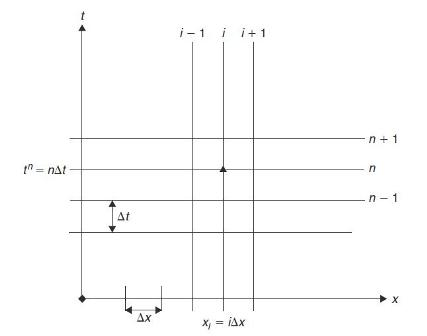
\includegraphics[scale=1]{figuras/espaco_tempo.jpg}
	\caption{\textsc{Discretização nos eixos espaço e tempo}}
	\vspace{-0.1cm}
	\legend{FONTE: \citeonline{Hirsch}}
	\label{fig:espaço_tempo}
\end{figure}

%\begin{figure}[h]
%\caption{DISCRETIZAÇÃO NOS EIXOS ESPAÇO E TEMPO}
%\label{fig:espaço_tempo}
%\centering
%\includegraphics[scale=1]{espaço_tempo.jpg}
%\end{figure} 

Conforme comentado em \citeonline{Press}, os métodos explícitos são de fácil implementação, pois a função é avaliada por meio de valores já conhecidos, o que os tornam muito econômicos em função do número de operações necessárias para avançar no tempo. Já para os esquemas implícitos, é necessário determinar três valores desconhecidos no tempo $n+1$, o que conduz a resolução de um sistema de equações tridiagonal, que pode ser linear ou não, dependendo da equação a ser resolvida. Para o caso de um sistema linear tridiagonal, o algoritmo de Thomas pode ser facilmente implementado. No entanto, para um sistema não linear o número de operações necessárias para o avanço no tempo pode ser muito maior.

De forma análoga ao que foi desenvolvido para as aproximações de segunda ordem no caso unidimensional, pode-se obter às aproximações de segunda ordem bidimensional, assunto amplamente discutido em literaturas como \citeonline{Tan} ou \citeonline{Leveque1992}.


\section{CONVERGÊNCIA, CONSISTÊNCIA E ESTABILIDADE} \label{Conver}

A falta de conhecimento das soluções exatas de certos problemas, nos remete à resolvê-los de forma aproximada por meio de um esquema ou método numérico. No entanto, faz-se necessário verificar até que ponto a forma numérica adotada é satisfatória para tal tarefa.

De acordo com \citeonline{Kundu}, a verificação da "qualidade" \ de um esquema numérico, seja ele implícito ou explícito, necessita de três conceitos: a convergência, a consistência e a estabilidade da solução numérica.

Segundo \citeonline{Crossley}, neste conjunto de conceitos ainda pode ser incluído a precisão, que define o quanto a solução aproximada está conseguindo representar da solução exata. Para tanto, se faz necessário o conhecimento de duas quantidades, que são: o erro local ou truncamento, que é a diferença entre a solução numérica em um dado ponto e a solução exata para este mesmo ponto, e o erro global, que reflete o erro total da solução numérica, o que quase sempre é impossível de se obter, já que a solução exata, no geral, é desconhecida.

Para \citeonline{Hirsch}, um esquema numérico é dito convergente quando a solução obtida tende para a solução exata no momento em que os passos, no tempo e no espaço, tendem para zero. Assim, o erro de truncamento pode ser definido como
\begin{equation}
\tilde{ \epsilon}^{n}_{i} = u^{n}_{i} - \tilde{ u} \left( i \Delta x , n \Delta t \right),
\end{equation}
onde $ \tilde{ u}(x,t)$ é a solução exata e, então, da condição de convergência, resulta que
\begin{equation}
\lim_{ \stackrel{ \Delta x \rightarrow 0}{ \Delta t \rightarrow 0} } | \tilde{ \epsilon}^{n}_{i} | = 0.
\end{equation}

\citeonline{Kundu} também afirmam que algumas medidas do erro podem ser estimadas por
\begin{equation}
\left\| e^{n}_{i} \right\| \leq k \Delta x^{a} \Delta t^{b} ,
\end{equation}
onde esta medida pode ser determinada como a raiz quadrada do erro médio, sendo $k$ uma constante que depende de $ \Delta x$ e $ \Delta t$, $a$ e $b$ são razões de convergência quando o erro se aproxima de zero.

Ao que foi visto acima, tudo leva a crer que um \textit{grid} pode ser reduzido indiscriminadamente e a convergência será sempre alcançada. No entanto, conforme afirma \citeonline{Crossley}, isto só será possível se o método for consistente, ou seja, ao ser reduzido o tamanho do passo no espaço e/ou no tempo a equação discretizada tender para a equação diferencial onde, neste caso, o método será dito como de uso prático.

Deve ser lembrado que, devido à aritmética finita dos computadores, pode haver um acúmulo no erro à medida que ocorre o avanço no tempo no processo de discretização. Se não houver um controle para este erro, a solução tenderá para o infinito e o método será dito instável. Portanto, um método será dito estável quando, ao avançar no tempo, mantiver o erro limitado. Isto é uma condição somente do método numérico utilizado e não envolve as condições da equação diferencial \cite{Hirsch}.

Muitos métodos numéricos tem o seu \textit{grid} limitado pelo número de Courant-Friedrichs-Lewy ($Co$),
\begin{equation} \label{CFL}
Co \leq 1
\end{equation}
o que indica que a partícula de um fluido não pode percorrer mais do que um \textit{grid} espacial em um passo de tempo.

Dentre os conceitos analisados, a estabilidade é decisiva para a viabilidade de uma aproximação numérica, devido ser uma condição necessária (em vez de suficiente) para se ter a precisão. A relação entre consistência, estabilidade e convergência é conhecida como o Teorema da Equivalência de Lax \cite{Hirsch}.
\begin{theorem}[Teorema de Lax]
	Dada uma equação diferencial parcial com condições iniciais e de contorno, bem postas, e um esquema de discretização que satisfaz à condição de consistência, então a estabilidade é uma condição necessária e suficiente para a convergência.
\end{theorem}

Pode-se adotar três procedimentos para a análise de estabilidade, que são: a estabilidade eurística, a estabilidade de Von Neumann e a estabilidade matricial. Destes, o mais utilizado, segundo \citeonline{Sperandio}, é a análise de Von Neumann que, basicamente, representa o erro numérico via uma decomposição harmônica de Fourier, ou seja,
\begin{equation} \label{Von_Neumann}
u^{n}_{j} = \xi ^{n} e^{ ikj \Delta x}, 
\end{equation}
onde $k$ é um número de onda espacial real e $ \xi = \xi (k)$ é um número complexo que depende de $k$, chamado de fator de amplificação. Em seguida, a decomposição harmônica é substituída na equação discretizada e, então, é feita a análise do crescimento do erro, determinando assim se o método é condicionalmente estável ou incondicionalmente estável. Mais detalhes do assunto podem ser vistos em \cite{Hirsch}, \cite{Kundu}, \cite{Sperandio} ou \cite{Batchelor}.

%-------------------------------------------------------------------------------------------------------------------------------------------------------
\section{O ESQUEMA DE LAX-FRIEDRICHS} \label{Lax_Fri}

Como mostrado anteriormente, a equação linear hiperbólica da advecção, equação (\ref{advecção}), foi discretizada por meio do MDFE, equação (\ref{explícito}). No entanto, a forma como foi construída esta discretização gera instabilidade que, segundo o Teorema de Lax, não será convergente. Nota-se isso por meio da análise de Von Neumann que, ao substituir o fator de amplificação (\ref{Von_Neumann}) na equação (\ref{explícito}), resulta
\begin{equation} \label{instabi}
\xi (k) = 1-i(Co)sen(k \Delta x),
\end{equation}
onde $ Co = {a \Delta t}/{ \Delta x} \leq 1$, é o número de Courant-Friedrichs-Lewy, desigualdade (\ref{CFL}), e $i$ é um número imaginário.

De acordo com \citeonline{Press}, como 
\begin{equation}
| \xi (k)| = |1-i(Co)sen(k \Delta x)| >1,
\end{equation}
para todo $k$, então o método é incondicionalmente instável. A Figura \ref{fig:Dias_A} mostra as instabilidades geradas para alguns intervalos de tempo.

\begin{figure}[H]
	\centering
	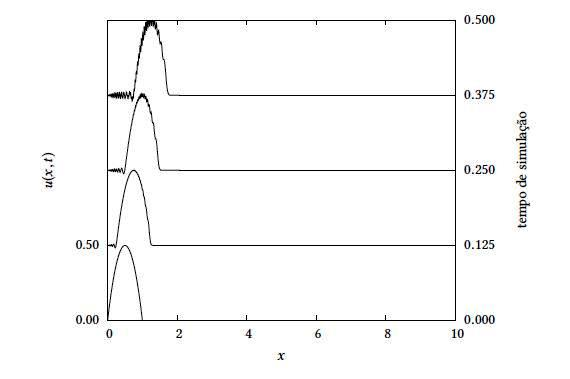
\includegraphics[scale=1]{figuras/Dias_A.jpg}
	\caption{\textsc{Solução numérica da equação da advecção por meio do MDFE}}
	\vspace{-0.1cm}
	\legend{FONTE: Autoria própria}
	\label{fig:Dias_A}
\end{figure}

Para tentar solucionar o problema da instabilidade o esquema de Lax-Friedrichs substitui o termo $u^{n}_{i}$, na equação (\ref{explícito}), por um termo médio, ou seja, 
\begin{equation} \label{ELF}
u^{n}_{i} = \frac{1}{2} \left( u^{n}_{i+1} + u^{n}_{i-1} \right).
\end{equation}
Dessa forma, a equação (\ref{explícito}) passa a ser escrita como
\begin{equation} \label{esq_Lax}
u^{n+1}_{i} =  \frac{1}{2} \left[ \left( u^{n}_{i+1} + u^{n}_{i-1} \right)  - (Co) \left( u^{n}_{i+1} - u^{n}_{i-1} \right) \right]. 
\end{equation} 

Ao fazer a análise de estabilidade de Von Neumann na equação (\ref{esq_Lax}) encontra-se que
\begin{equation} \label{instabi_Lax}
\xi (k) = cos(k \Delta x)-i(Co)sen(k \Delta x).
\end{equation}

Se $ \xi (k)$ na equação (\ref{instabi_Lax}), que é um número complexo, for maior do que $1$, então o esquema (\ref{esq_Lax}) será instável, mas se for considerado que $ | \xi (k)|^{2} \leq 1$ o esquema (\ref{esq_Lax}) será estável, o que só será possível se $Co \leq 1$, que é o critério de Courant-Friedrichs-Lewy.

Segundo \citeonline{Press}, o que ocorre no esquema de Lax-Friedrichs é a inclusão de um termo difusivo, ou seja, o esquema de Lax-Friedrichs é dito ter uma dissipação numérica ou viscosidade numérica. Isto pode ser observado na Figura \ref{fig:Dias_B}, onde não ocorre mais as soluções espúrias que estavam ocorrendo na Figura \ref{fig:Dias_A}, mostrando que o esquema (\ref{esq_Lax}) é estável. No entanto, a solução é "amortecida" \ pela difusão numérica, o que pode prejudicar a resposta do ponto de vista físico do problema. Existem outras forma de contornar o problema da instabilidade encontrada pelo MDFE, como o método de Lax-Wendroff ou mesmo o esquema Upwind, mas não serão abordados neste trabalho. Tais métodos podem ser encontrados em literaturas como \citeonline{Press}, \citeonline{Hirsch}, \citeonline{Kundu}, \citeonline{Sperandio} ou \citeonline{Batchelor}.

\begin{figure}[H]
	\centering
	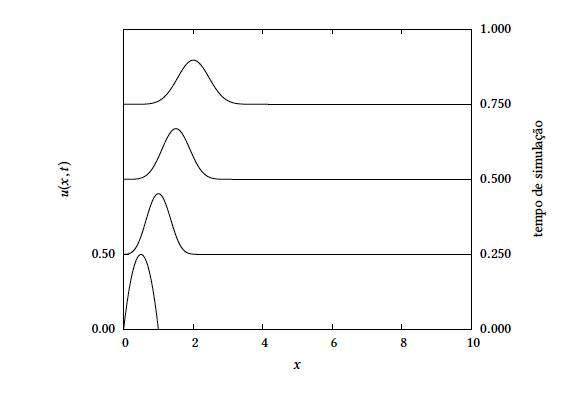
\includegraphics[scale=1]{figuras/Dias_B.jpg}
	\caption{\textsc{Solução numérica da equação da advecção por meio do esquema de Lax-Friedrichs}}
	\vspace{-0.1cm}
	\legend{FONTE: Autoria própria}
	\label{fig:Dias_B}
\end{figure}
%-------------------------------------------------------------------------------------------------------------------------------------------------------

\section{MÉTODO DAS CARACTERÍSTICAS} \label{Caracteristicas}

Define-se como "características" \ linhas no plano espaço-tempo ao longo das quais certas propriedades das Equações Diferenciais Parciais (EDPs) se propagam e o método pode ser considerado como uma forma analítica de obter suas soluções \cite{Cunge}.

Utilizando como exemplo a EDP de primeira ordem
\begin{equation}\label{exempcarac}
u_t +a(x,t)u_x=0,
\end{equation}
com condição inicial $u(x,0)=u_0$. Pode-se definir, pela regra da cadeia \cite{Leithold}, que
\begin{equation*}
\frac{du}{dt} = u_t + \frac{dx}{dt}u_x,
\end{equation*}
ou seja, 
\begin{equation} \label{uisolado}
u_t = \frac{du}{dt} - \frac{dx}{dt}u_x.
\end{equation}

Substituindo a equação (\ref{uisolado}) na equação (\ref{exempcarac}) defini-se que
\begin{equation} \label{CaracIsol}
\frac{du}{dt} + \left( a(x,t) -\frac{dx}{dt} \right)u_x = 0.
\end{equation}

Observando a equação (\ref{CaracIsol}) percebe-se que ${du}/{dt} = 0$ em toda linha definida por ${dx}/{dt} = a(x,t)$. Isso implica que a solução $u$ é constante ao logo daquela linha, conhecida como linha característica.

Se for possível definir um conjunto de linhas características, então será possível conhecer a solução para todos os tempos, sendo necessário para isso apenas as condições iniciais e as condições do contorno do problema, desde que as linhas não se interceptem. Assim, pode-se obter a solução do problema, equação (\ref{exempcarac}), por
\begin{equation}
u(x,t) = u \left( x - \int\limits_{0}^{t} a(x,t) dt , 0 \right).
\end{equation}  

Considerando o domínio do problema uma região finita, conforme a Figura \ref{fig:dominiofinito}, para obter uma solução é necessário especificar os valores ao longo de alguma fronteira que contém as linhas características. Por exemplo, se for especificado o valor ao longo da linha $x=x_1$, não será necessário especificar os valores das demais linhas, pois as linhas características, dentro da região finita, já serão conhecidas.

\begin{figure}[H]
\centering
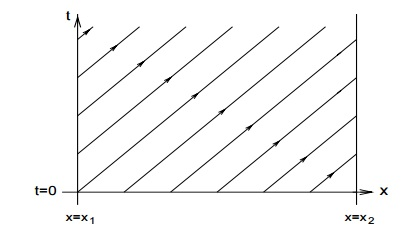
\includegraphics[scale=1.2]{figuras/Caracteristica.jpg}
\caption{\textsc{Linhas características sobre um domínio finito}}
\vspace{-0.1cm}
\legend{FONTE: \citeonline{Crossley}}
\label{fig:dominiofinito}
\end{figure}


Se for considerado o caso em que
\begin{equation}
u_t + a(u)u_x = 0,
\end{equation}
onde $ f'(u) = a(u)$, então
\begin{equation}
u_t + f(u)_x = 0
\end{equation}
será uma lei de conservação escalar, sendo a característica dada por
\begin{equation}
\frac{dx}{dt} = a(u).
\end{equation}

Definido $u$ como constante ao longo da linha característica acima, $a$ também será constante, sendo que todas as características serão linhas retas e, pela teoria das Equações Diferenciais Ordinárias (EDOs) \cite{kreyszig}, será possível mostrar que, para $u$ contínuo, as linhas características não irão se interceptar. No entanto, as EDPs hiperbólicas admitem soluções descontínuas e, para uma lei de conservação hiperbólica não linear, as linhas características irão se interceptar formando descontinuidades ou choques, como pode ser observado nas interpretações geométricas construídas no trabalho de \citeonline{Adilandri}.

%-------------------------------------------------------------------------------------------------------------------------------------------------------
\section{HIDRODINÂMICA DE PARTÍCULAS SUAVIZADAS} \label{Hidro_SPH}

Além do MDF, outra ferramenta da CFD são os métodos lagrangeanos sem malhas baseados em partículas (\textit{meshfree methods}). Estes tipos de métodos vêm ganhando espaço na modelagem computacional, principalmente com a melhora na capacidade de processamento dos computadores e com a crescente programação direta em placas gráficas, como pode ser visto no trabalho de \citeonline{Harada}.

De acordo com \citeonline{Queiroz}, estes métodos possuem a vantagem de se adaptarem a grandes deformações, de suportarem mudanças topológicas e de lidarem de forma "robusta" \ com os refinamentos adaptativos para o controle da precisão dos resultados. Em contrapartida, possuem como principal desvantagem o custo computacional na busca por partículas vizinhas, já que necessitam das informações particulares de cada uma delas para avançar no tempo.

Dentre os métodos sem malhas existentes, o Método das Partículas Suavizadas ( \textit{Smoothed Particle Hydrodynamics}-SPH), se destaca nas simulações de escoamentos de fluidos, pois permite estas realizações em tempo linear, o que é desejável para aplicações em tempo real (\citeonline{Muller}, \textit{apud} \citeonline{Queiroz}).

O SPH surgiu para modelar fenômenos astrofísicos nos trabalhos desenvolvidos por \citeonline{Lucy} e \citeonline{Gingold}. A ideia básica deste método consiste em substituir o domínio físico por um domínio discretizado por meio de partículas (núcleos), onde cada um destes núcleos possui propriedades como pressão, densidade, velocidade, etc. Para cada ponto do domínio, a função ou uma de suas derivadas é aproximada por uma média ponderada das contribuições de todas as partículas que estão próximas deste ponto, ou seja, é feita uma convolução, conforme comentado em \citeonline{Paiva2009}. Assim, dada uma função $f$ definida sobre um volume $\Omega$, tem-se:
\begin{equation} \label{integral}
f(\textbf{r}) = \int_{\Omega} f(\textbf{r'})\delta(\textbf{r}-\textbf{r'})dr',
\end{equation}
onde $\delta$ é a função Delta de Dirac, $\textbf{r}$ e $\textbf{r'}$ são variáveis no domínio de $\Omega$.

Da definição da função Delta de Dirac, \cite{Queiroz}, tem-se
\begin{equation}
\delta = \left\{
\begin{array}{rcl}
1 & se & \textbf{r} = \textbf{r'}\\
0 & se & \textbf{r} \neq \textbf{r'}
\end{array} \right.
\end{equation}
e
\begin{equation}
\int_{\Omega} \delta(\textbf{r}-\textbf{r'})dr =1.
\end{equation}

Apesar do uso da função Delta de Dirac na equação (\ref{integral}), isto é apenas uma função generalizada, pois nenhuma função pode ter as mesmas propriedades que ela. Desta forma, pode-se afirmar que a equação (\ref{integral}) não é compatível e deve-se substituir a função Delta de Dirac por uma função que se comporte como ela. Tal função é a função núcleo suavizado (\textit{Smooth Kernel}) $W(\textbf{r},h)$, onde $h$ é o comprimento de suavização (\textit{Smooth Lenght}), devendo satisfazer as seguintes propriedades:
\begin{enumerate}
	\item[1)] $W$ deve se aproximar do comportamento da função $\delta$ quando $h$ tende para zero, o que garante a consistência da equação (\ref{integral})
	\begin{equation}
	\lim\limits_{h \rightarrow 0} W(\textbf{r},h) = \delta(\textbf{r}).
	\end{equation}
	
	\item[2)] Assim como a função $\delta$, $W$ deve ser normalizada
	\begin{equation}
	\int_{\Omega} W(\textbf{r},h) dr' = 1.
	\end{equation}
	
	\item[3)] A função núcleo deve possuir um suporte compacto, ou seja, deve ser nula sempre que o comprimento for maior do que $kh$, sendo $k$ uma constante relacionada com o comprimento de suavização
	\begin{equation}
	W(\textbf{r},h) = 0 ; |\textbf{r} - \textbf{r'}| > kh.
	\end{equation}
	
	\citeonline{Paiva2009} destaca ainda que a função núcleo deve satisfazer mais três propriedades, que são:
	\item[4)] O núcleo deve ser sempre positivo no suporte compacto, pois se for negativo pode afetar a densidade
	\begin{equation}
	W(\textbf{r},h) \geq 0.
	\end{equation}
	
	\item[5)] O núcleo deve ser sempre decrescente, ou seja, as partículas mais distantes do núcleo central tem menor influência sobre ele
	\begin{equation}
	W(\textbf{x},h) < W(\textbf{r},h)  \\ se \\ \parallel \textbf{x} \parallel > \parallel \textbf{r} \parallel.
	\end{equation}        
	
	\item[6)] O núcleo deve ser simétrico, o que pode ser mostrado por meio da expansão de $W(\textbf{r} - \textbf{r'},h)$ por série de Taylor \cite{Monaghan1992}
	\begin{equation}
	W(\textbf{r} - \textbf{r'},h) = W(\textbf{r'} - \textbf{r},h).
	\end{equation}
\end{enumerate}

Satisfeitas as propriedades anteriores, substituindo o volume infinitesimal $dr'$ por um volume finito $\Delta V$, representado por partículas vizinhas, e relacionado este volume com a massa $m$ de uma das partícula por meio da expressão $m= \Delta V \cdot \rho$, então a equação (\ref{integral}) pode ser discretizada por
\begin{equation} \label{aprox_SPH}
f(\textbf{r}) \approx \sum\limits_{i} \frac{m_{i}}{\rho_{i}} f(\textbf{r}_{i}) W(\textbf{r} - \textbf{r}_{i},h),
\end{equation} 
onde $i$ é uma distância sobre todas as partículas próximas ao núcleo suavizado. As Figuras \ref{fig:nucleo_B} e \ref{fig:nucleo_A} mostram esquemas representativos da função núcleo, sendo que na Figura \ref{fig:nucleo_A} tem-se ainda a representatividade da influência que as partículas vizinhas exercem sobre o núcleo.

\begin{figure}[H]
	\centering
	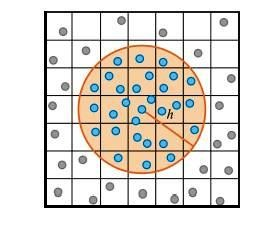
\includegraphics[scale=1]{figuras/nucleo_B.jpg}
	\caption{\textsc{Representação do núcleo no suporte compacto}}
	\vspace{-0.1cm}
	\legend{FONTE: \citeonline{Bruno}}
	\label{fig:nucleo_B}
\end{figure}

\begin{figure}[H]
	\centering
	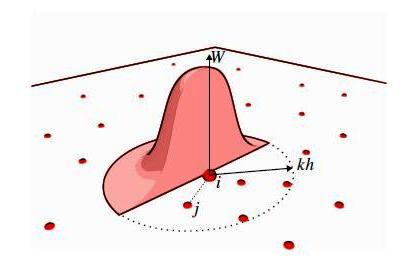
\includegraphics[scale=1]{figuras/nucleo_A.jpg}
	\caption{\textsc{Representação do núcleo no suporte compacto sob a influência das partículas dentro do raio $kh$}}
	\vspace{-0.1cm}
	\legend{FONTE: \citeonline{Queiroz}}
	\label{fig:nucleo_A}
\end{figure}       

A forma como a função $f$ foi discretizada na equação (\ref{aprox_SPH}) para uma posição $\textbf{r}$, num domínio computacional $\Omega$, é a base de todo o formalismo do SPH.

Como visto nas propriedades, a escolha do núcleo é importante para a correta discretização da função $f$ e diferentes funções podem ser utilizadas para cumprir tal tarefa. \citeonline{Gingold} propuseram, como função núcleo, a função gaussiana
\begin{equation}
W(\textbf{r} - \textbf{r'},h) = \frac{1}{h^{3} \pi^{3/2}} e^{-x^{2}},
\end{equation}
sendo, $x = {| \textbf{r} - \textbf{r'}|}/{h}$. No entanto, esta função não possui suporte compacto, mas aproxima-se rapidamente de zero, sem nunca atingi-lo, quando as distâncias entre duas partículas aumenta. Assim, ocorrerá a inclusão de muitas partículas na vizinhança, conforme a Figura \ref{fig:nucleo_B}, o que terá um custo computacional alto demais.

Outro tipo de função amplamente utilizada são as funções Splines. No trabalho de \citeonline{Monaghan1985} foi proposto o uso da função spline cúbica  
\begin{equation}
W(\textbf{r} - \textbf{r'},h) = \frac{1}{\pi h^{3}} \left\{
\begin{array}{rcl}
1 - \frac{3}{2} x^{2} + \frac{3}{4} x^{3} & se & 0 \leq x < 1 \\
\frac{1}{4}(2-x)^{3} & se & 1 \leq x < 2 \\
0 & se & x \geq 2,  
\end{array} \right.
\end{equation}
onde somente partículas que distam $2h$ do centro contribuem para a suavização do núcleo. Splines de maior grau também são utilizadas para aproximação do núcleo, bem como outras variações, como aquelas propostas no trabalho de \citeonline{Lucy}. No entanto, todas apresentam problemas em satisfazer as propriedades necessárias. A Figura \ref{fig:nucleos} mostra o comportamento de três núcleos, sendo que o núcleo spline cúbico é o que melhor se compara com o gaussiano, por isso é o mais utilizado. Já a Figura \ref{fig:pricePDF4} mostra o comportamento de outras funções spline representando o núcleo. Mais detalhes sobre as funções núcleo podem ser encontrados na bibliografia como \citeonline{Paiva2009} ou  \citeonline{Violeau}.

\begin{figure}[H]
	\centering
	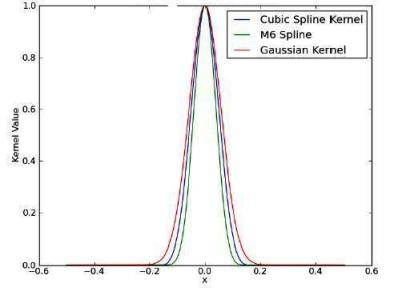
\includegraphics[scale=1]{figuras/nucleos.jpg}
	\caption{\textsc{Comparação das funções splines de terceiro e quinto graus com a função gaussiana}}
	\vspace{-0.1cm}
	\legend{FONTE: \citeonline{CodigoPySPH}}
	\label{fig:nucleos}
\end{figure} 

\begin{figure}[H]
	\centering
	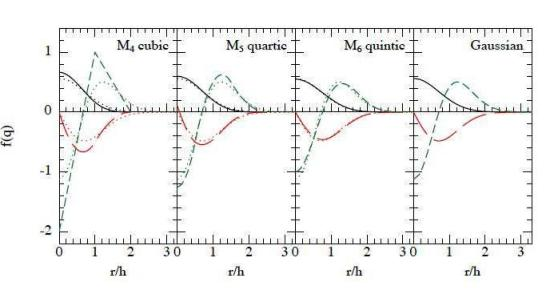
\includegraphics[scale=1]{figuras/pricePDF4.jpg}
	\caption{\textsc{Comparação das funções splines de terceiro, quarto e quinto graus e suas derivadas, primeira e segunda, linhas pontilhadas longas e curtas, respectivamente, com a função gaussiana}}
	\vspace{-0.1cm}
	\legend{FONTE: \citeonline{Price}}
	\label{fig:pricePDF4}
\end{figure} 

Uma vez determinado o núcleo, a modelagem por meio do SPH necessita das derivadas de alguns campos, como os vetoriais e escalares. Assim, considerando a equação (\ref{integral}) como um campo escalar, seu gradiente pode ser avaliado por
\begin{equation}
\nabla f(\textbf{r}) = \frac{\partial}{\partial \textbf{r}} \int\limits_{\Omega} f({\textbf{r'}) \delta (\textbf{r} - \textbf{r'})}dr',
\end{equation}  
cuja aproximação, por intermédio de (\ref{aprox_SPH}) , resulta em
\begin{equation} \label{esc_SPH}
\nabla f(\textbf{r}) \approx \sum\limits_{i} \frac{m_{i}}{\rho_{i}} f(\textbf{r}_{i}) \nabla W(\textbf{r} - \textbf{r}_{i},h).
\end{equation}

Se a equação (\ref{integral}) for considerada como um campo vetorial, $\vec{F(\textbf{r})}$, então
\begin{equation}
\vec{F(\textbf{r})} = \int\limits_{V} \vec{F(\textbf{r'})} \delta (\textbf{r} - \textbf{r'})dr'.
\end{equation} 
Assim, calculando o seu divergente em relação à $\textbf{r}$, a aproximação integral torna-se
\begin{equation} \label{div_SPH}
\nabla \cdot \vec{F(\textbf{r})} \approx \sum\limits_{i} \frac{m_{i}}{\rho_{i}} \vec{F(\textbf{r}_{i})}  \cdot \nabla W(\textbf{r} - \textbf{r}_{i},h). 
\end{equation}

De forma análoga, pode-se determinar o rotacional do campo vetorial $\vec{F(\textbf{r})}$, ou seja, $\nabla \times \vec{F(\textbf{r})}$ sendo aproximado por
\begin{equation} \label{rot_SPH}
\nabla \times \vec{F(\textbf{r})} \approx \sum\limits_{i} \frac{m_{i}}{\rho_{i}} \vec{F(\textbf{r}_{i})}  \times \nabla W(\textbf{r} - \textbf{r}_{i},h).
\end{equation}

Conforme comentado em \citeonline{Paiva2009}, alguns destes operadores são imprecisos e podem não obedecer as propriedades de conservação quando utilizados na simulação do escoamento de fluidos. Deste forma, existem variações das aproximações dos campos escalares e vetoriais. Os erros destas aproximações, bem como outras formas de aproximar os gradientes e divergentes daqueles campos, podem ser encontrados em \citeonline{Monaghan1992}.

A representação do escoamento de um fluido, por meio da discretização do SPH, inicia-se com a representação da densidade de uma partícula específica $\rho_{j}$, diretamente da aproximação (\ref{aprox_SPH}). Assim, pode-se considerar que
\begin{equation}
\rho_{j} = \sum\limits_{i} m_{i} W(\textbf{r}_{j} - \textbf{r}_{i},h)
\end{equation}
ou, de forma simplificada,
\begin{equation} \label{Densi_PSH}
\rho_{j} = \sum\limits_{i} m_{i} W_{ji}.
\end{equation} 

Novamente por \citeonline{Paiva2009}, o cálculo da densidade usando a equação aproximada (\ref{Densi_PSH}) exige um esforço adicional na implementação numérica, pois a densidade deve ser calculada em primeiro lugar para todas as partículas, antes dos demais parâmetros. Uma alternativa é a substituição de uma das formas dos divergentes, como a equação (\ref{div_SPH}), diretamente na equação da continuidade (\ref{eq_massa_2}), o que resulta 
\begin{equation} \label{Cont_SPH}
\frac{d \rho_{j}}{dt} = -\rho_{j} \sum\limits_{i} \frac{m_{i}}{\rho_{i}} (\textbf{v}_{i} - \textbf{v}_{j}) \cdot \nabla_{j}W_{ji},
\end{equation}
que é a equação da Continuidade na formulação SPH, onde $\textbf{v}_{i} = {d \textbf{r}_{i}}/{dt}$ e $\textbf{v}_{j} = {d \textbf{r}_{j}}/{dt}$.

De acordo com \citeonline{Cossins}, como a discretização é feita sob uma dada partícula em um meio contínuo, pode ser considerada a derivada total para determinar a equação da Continuidade, conforme mostrado na equação (\ref{Cont_SPH}). Assim, também para a equação de Conservação do Movimento (\ref{eq_movimento_final}), a aproximação SPH é dada por
\begin{equation} \label{Mov_SPH}
\frac{d \textbf{v}_j}{dt} = -\sum\limits_{i}m_{i} \left( \frac{P_j}{\rho^{2}_{j}} + \frac{P_i}{\rho^{2}_{i}} \right) \nabla_{j}W_{ji}.
\end{equation}

Para a equação da Energia Total (\ref{Energi_T}),  a aproximação SPH é dada por
\begin{equation} \label{energ_SPH}
E = \sum\limits_{i} m_{i} \left( \frac{1}{2} \textbf{v}_{i} \cdot \textbf{v}_{i} + e_{i} \right),
\end{equation}
cuja derivada no tempo resulta em
\begin{equation}
\frac{dE}{dt} = \sum\limits_{i} \sum\limits_{j}  m_{i}  m_{j} \left( \frac{P_j}{\rho^{2}_{j}} \textbf{v}_{i} +  \frac{P_i}{\rho^{2}_{i}} \textbf{v}_{j} \right) \cdot \nabla_{j}W_{ji} 
\end{equation}
que, novamente por \citeonline{Cossins}, é conservativa.

A implementação computacional usando o método SPH deve seguir uma sequência lógica de operações, já que cada partícula transporta consigo propriedades físicas inerentes ao fluido que está sendo modelado e, a cada passo de tempo, sofre a influência das demais partículas que estão no seu suporte compacto. Além do mais, com o avanço no tempo, as posições não são preservadas, fazendo com que a simulação total sofra constantes atualizações. Desta forma, se o algoritmo não for eficiente, capaz de "prever" \ estas particularidades do método, acabará comprometendo a simulação.

No trabalho de \citeonline{Paiva2009} é apresentado um visão simplificada da implementação por meio do SPH, conforme pode ser observado na Figura \ref{fig:visao}. Deste esquema simplificado destacam-se dois pontos principais que podem afetar a simulação, que são: a busca por partículas vizinhas e as condições de fronteira.
\begin{figure}[H]
	\centering
	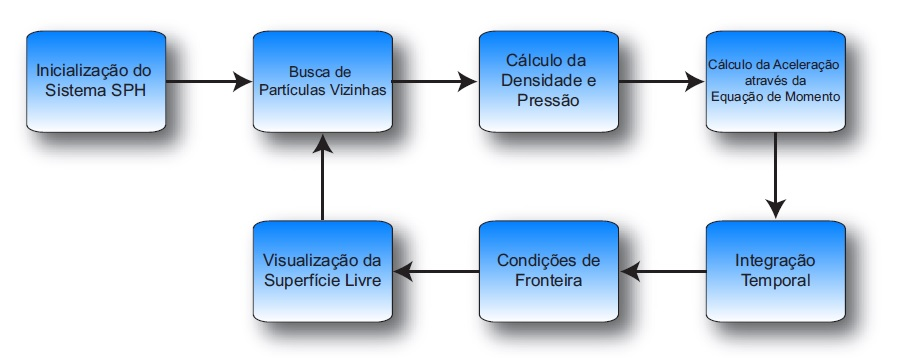
\includegraphics[scale=0.9]{figuras/visao.jpg}
	\caption{\textsc{Visão simplificada da implementação computacional usando o SPH}}
	\vspace{-0.1cm}
	\legend{FONTE: \citeonline{Paiva2009}}
	\label{fig:visao}
\end{figure}

No SPH as partículas estão sempre mudando de posição, então é necessário uma atualização constante dos vizinhos de cada núcleo. Um dos métodos utilizados para realizar esta tarefa é o da Força Bruta, que verifica quais as partículas estão a uma distância inferior a $kh$ de um determinado núcleo e as considera no suporte compacto. É um método simples, mas pode ser muito custoso, pois a medida que o número $n$ de partículas aumenta exige um esforço computacional maior, já que eleva o tempo computacional à ordem $O(n^2)$. Outras formas adotadas para determinar as partículas vizinhas são as Buscas em Grades, Figura \ref{fig:grade}, e a Busca por Estruturas Adaptativas, particularizada pelas estruturas \textit{kd-tree} e \textit{octree}, Figura \ref{fig:octree}. Cada uma delas apresentam vantagens e desvantagens, dependendo da simulação desejada, conforme pode ser visto na bibliografia como \citeonline{Capone}.
\begin{figure}[H]
	\centering
	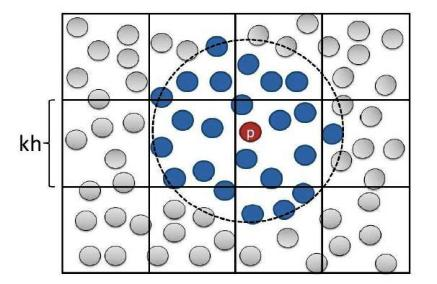
\includegraphics[scale=1]{figuras/grade.jpg}
	\caption{\textsc{Determinação das partículas vizinhas pelo método de Busca em Grades}}
	\vspace{-0.1cm}
	\legend{FONTE: \citeonline{Violeau}}
	\label{fig:grade}
\end{figure}
\begin{figure}[H]
	\centering
	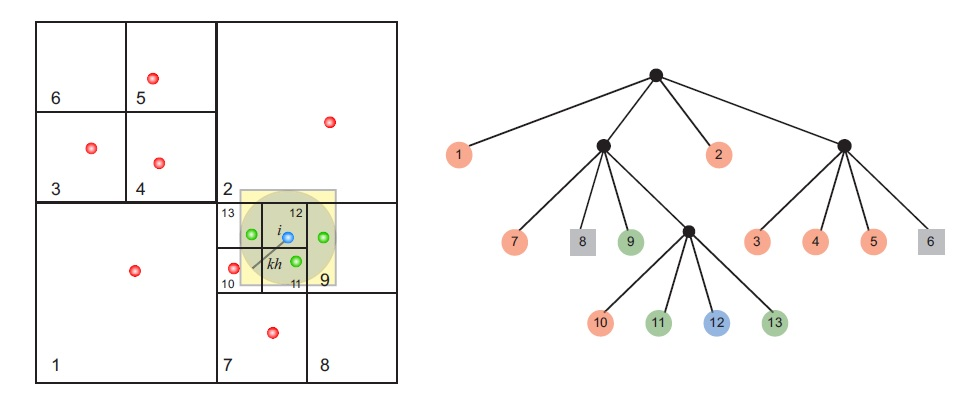
\includegraphics[scale=.8]{figuras/octree.jpg}
	\caption{\textsc{Determinação das partículas vizinhas usando Estruturas Adaptativas como as estruturas octree}}
	\vspace{-0.1cm}
	\legend{FONTE: \citeonline{Paiva2009}}
	\label{fig:octree}
\end{figure}

Para as condições de fronteira, existe a necessidade de manter o fluido, de certa forma, "confinado". Para tanto, há o método das Partículas Fantasmas, onde as fronteiras são partículas capazes de gerar forças de repulsão e de manter as demais partículas dentro do domínio desejado. Para tanto, as partículas são dispostas ao longo da fronteira com o intuito de repelir as partículas internas que se aproximam do contorno, conforme pode ser observado da Figura \ref{fig:particula_fantasma} que esquematiza este processo. No entanto, este tratamento pode ser difícil de ser mantido para geometrias mais complexas, conforme abordado no trabalho de \citeonline{Vacondio}.
\begin{figure}[H]
	\centering
	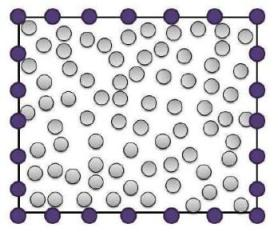
\includegraphics[scale=1]{figuras/particula_fantasma.jpg}
	\caption{\textsc{Tratamento das fronteiras usando Partículas Fantasmas}}
	\vspace{-0.1cm}
	\legend{FONTE: \citeonline{Queiroz}}
	\label{fig:particula_fantasma}
\end{figure} 

Para geometrias mais complexas, \citeonline{Paiva2007} propôs um método baseado na Reflexão Geométrica, Figura \ref{fig:colisao}, onde as partículas que irão colidir com a fronteira, partícula $t_0$, tem sua trajetória e velocidade corrigida, partícula $t_1$, como se realmente tivesse entrado em contato com a fronteira.
\begin{figure}[H]
	\centering
	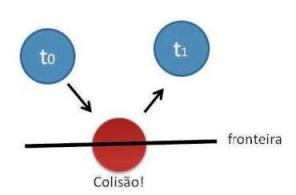
\includegraphics[scale=1]{figuras/colisao.jpg}
	\caption{\textsc{Tratamento das fronteiras usando Reflexão Geométrica}}
	\vspace{-0.1cm}
	\legend{FONTE: \citeonline{Queiroz}}
	\label{fig:colisao}
\end{figure}  

O assunto sobre o método SPH é amplo e seu uso tem evoluído nas mais diversas áreas do conhecimento e entretenimento, como bem destacado no trabalho de \citeonline{Paiva2009}. Junto com essa evolução estão os algoritmos que simulam as mais variadas geometrias e formas de escoamentos destacando-se, entre eles, o algoritmo proposto por \citeonline{Ramachandran2010}, intitulado PySPH, que será discutido no próximo capítulo.  



\chapter{ANÁLISE DE RUPTURA DE BARRAGENS}
%Título Capítulo 5 

Como pôde ser observado nos capítulos anteriores, a ruptura de barragens possui, além de aplicações práticas, importância científica. Neste contexto, este capítulo faz uma análise sobre esse fenômeno iniciando com uma visão geral sobre o assunto, Seção \ref{visao}. Prossegue destacando o trabalho de \citeonline{Crespo}, Seção \ref{arte}. Destaca a construção de um modelo unidimensional baseado nas equações de Euler, Seção \ref{Modelo1D} e obtém uma solução analítica unidimensional para as equações de Águas Rasas, Seção \ref{ModeloAR}. Depois, Seção \ref{py}, disserta sobre o código numérico PySPH, como foi realizado o tratamento de uma barragem hipotética e os resultados obtidos. Por fim, descreve como o assunto foi abordado nesta dissertação, Seção \ref{proposta} e a forma como foi desenvolvida a malha computacional, Seção \ref{malha}. 
    

\section{VISÃO GERAL DE UMA BARRAGEM HIPOTÉTICA} \label{visao}

Considerando seu valor científico, a modelagem da ruptura de uma barragem hipotética tem sido útil como forma de validação de muitos algoritmos numéricos, assim como foi feito no trabalho de \citeonline{CrespoBondary}.

Uma barragem pode ser representada como um tanque que, em seu interior, separa dois níveis de água. O nível com maior volume representa o reservatório (montante) e o de menor nível representa o leito do rio (jusante). Como exemplo desta representatividade pode-se destacar o trabalho realizado por \citeonline{Stansby} que construíram, em laboratório, um reservatório com diferentes níveis de água e capturaram, por meio de uma câmera de vídeo, os estágios iniciais da frente de onda formada pelo colapso daquela estrutura, Figura \ref{fig:captura}.

\begin{figure}[H]
\centering
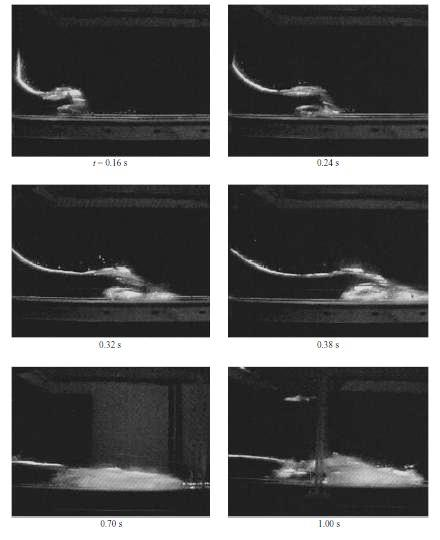
\includegraphics[scale=1]{figuras/captura.jpg}
\caption{\textsc{Captura dos estágios iniciais da simulação da ruptura de uma barragem em laboratório}}
\vspace{-0.1cm}
\legend{FONTE: \citeonline{Stansby}}
\label{fig:captura}
\end{figure}

Experimentos como esse são denominados de modelagem em "leitos úmidos", pois a jusante da barragem há uma fina camada de água, representado o leito do rio, no qual se deposita a água do reservatório no momento da falha da estrutura que as separa. Ao contrário disso, quando a jusante da barragem o leito não contém nenhuma lâmina d'água, denomina-se "leito seco". \citeonline{Korobkin} estudaram os estágios iniciais desse fenômeno e o resolveram analiticamente para pequenos intervalos de tempo, com o intuito de verificar o comportamento da linha de frente da coluna d'água. 

Em ambos experimentos os autores definiram a simulação da ruptura de barragens como uma massa líquida que, inicialmente em repouso, entra em movimento sob os efeitos da gravidade. Como os campos de pressões são diferentes, à montante um campo de pressão hidrostática, equação (\ref{eqhidro}), e à jusante a pressão atmosférica, no caso de um leito seco, ocorre um ajustamento entre eles, resultando em movimentos instáveis, conforme destacam \citeonline{Stansby}.

Quando a simulação é feita sob a hipótese de um leito úmido, a pressão a jusante também é hidrostática, mas as variações são menores devido à profundidade do leito. Neste caso, o comportamento da coluna d'água que se deposita sobre o leito do rio forma o que os pesquisadores denominam de frente de onda ou de inundação, largamente estudada pelos interessados em verificar o comportamento de ondas que atingem regiões costeiras ou por aqueles que desejam obter respostas sobre erosões que esses fenômenos pode causar em estruturas localizadas em regiões de risco. A Figura \ref{fig:stans6} mostra a formação dessas ondas para diferentes intervalos de tempo, destacando o contraste do fenômeno para diferentes profundidades do leito e, também, quando o leito é considerado seco.    

\begin{figure}[H]
\centering
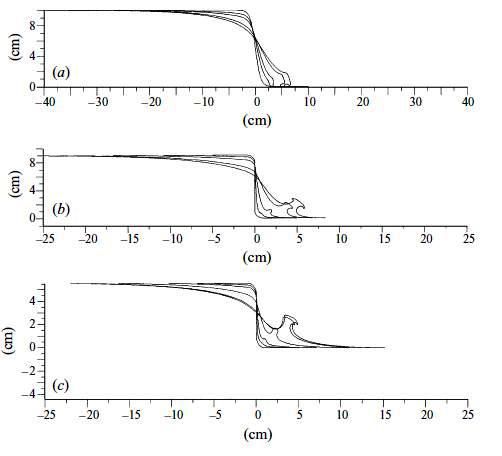
\includegraphics[scale=1]{figuras/stans6.jpg}
\caption{\textsc{Perfil da superfície de elevação para um escoamento potencial não linear em diferentes intervalos de tempo e profundidades}}
\vspace{-0.1cm}
\legend{FONTE: \citeonline{Stansby}}
\label{fig:stans6}
\end{figure}

A forma de tratar as condições iniciais e de contorno podem variar de acordo com a configuração adotada, seja euleriana ou lagrangeana, assim como a inserção de efeitos viscosos ou variações nas densidades. Para o caso de uma simulação usando SPH, por exemplo, existe a necessidade da adoção de uma viscosidade artificial que previna as instabilidades no movimento dos fluidos \cite{Monaghan1992}. Isso faz com que o tratamento das equações governantes do sistema varie em cada configuração e, também, dentro de uma mesma configuração, mas conduz a resultados quase sempre satisfatórios.  

%-------------------------------------------------------------------------------------------------------------------------------------------------------
\section{O ESTADO DA ARTE} \label{arte}

Para simular a ruptura de uma barragem hipotética utilizando as equações de Euler, discretizadas pelo MDFE, foi utilizado, como referência, o trabalho desenvolvido por \citeonline{Crespo}, onde autores estudaram a formulação clássica do SPH para problemas de escoamentos em superfícies livres investigando as variações de filtros de densidade, núcleos, as correções dos gradientes, viscosidades e as condições de fronteiras, como as partículas fantasmas e as partículas dinâmicas. 

Para testar seus resultados consideraram a barragem hipotética adotada por \citeonline{Koshizuka}, sendo que essa é montada em um tanque bidimensional com $4 \ m$ de comprimento, $3 \ m $ de altura e possui uma coluna d'água com $1 \ m$ de comprimento e $2 \ m$ de altura que simula o reservatório. A Figura \ref{fig:tanque} mostra a configuração inicial do sistema que, conforme pode ser observado, foi considerado como uma simulação para leito seco.

\begin{figure}[H]
\centering
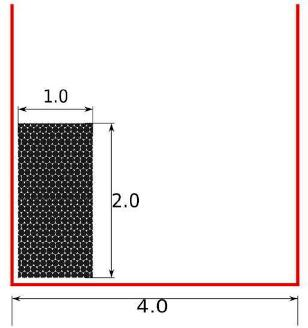
\includegraphics[scale=1]{figuras/tanque.jpg}
\caption{\textsc{Configuração inicial da coluna d'água e do tanque}}
\vspace{-0.1cm}
\legend{FONTE: \citeonline{Crespo}}
\label{fig:tanque}
\end{figure}

\citeonline{Crespo} resolveram o sistema utilizando um algoritmo preditor-corretor descrito no trabalho de \citeonline{Monaghan1989}. Consideraram núcleos formados pelas funções Spline cúbicas, condições de fronteira dinâmica, viscosidade artificial, $\alpha = 0,5$, e fator de correção XSPH, $\epsilon = 0,5$, que calcula uma média entre as velocidades das partículas vizinhas permitindo um escoamento mais suave e evitando a desordem entre as partículas \cite{Paiva2009}.

Como primeira simulação, consideraram um caso padrão adotando a discretização nos eixos coordenados $x$ e $z$ como $dx=dz=0,012 \ m$, tamanho da suavização do núcleo igual a $h=0,0156 \ m$, formando $29.723$ partículas, sem filtro de densidade ou fator de correção. A Figura \ref{fig:colapso} mostra a evolução das velocidades da coluna d'água para diferentes intervalos de tempo, destacando as velocidades no fundo, próximas da barragem, que são máximas. Destacam também, a formação do \textit{sloshing} quando ocorre a colisão com o muro direito.

\begin{figure}[H]
\begin{center}
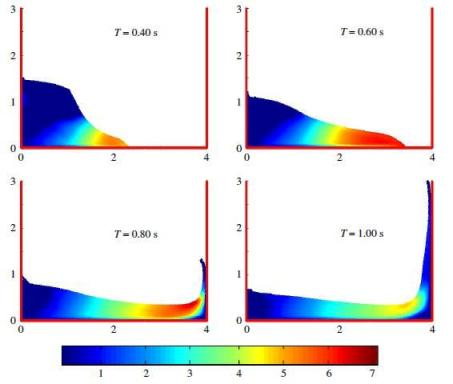
\includegraphics[scale=1]{figuras/colapso.jpg}
\end{center}
\caption{\textsc{Simulação em SPH das velocidades das partículas no colapso de uma coluna d'água}}
\vspace{-0.1cm}
\legend{FONTE: \citeonline{Crespo}}
%\fonte{\citeonline{Crespo}}
\label{fig:colapso}
\end{figure}   

Mais alguma conclusões são obtidas com este experimento, principalmente no que se refere as oscilações de pressão que, segundo os autores, podem ser suavizadas com o uso de filtros sobre a densidade. Assim, a Figura \ref{fig:sfiltro} destaca as variações da densidade em três intervalos de tempo, enfatizando o momento em que a massa líquida entra em contato com o muro, onde ocorre o maior aumento na densidade, $T=0,70s$, e, consequentemente, uma rápida queda de pressão que pode desestruturar os cálculos em todos os campos considerados. No entanto, com a utilização de filtros de densidade, conseguiram melhorar estas diferenças, sem muita interferência na forma física do problema, como pode ser notado nas Figuras \ref{fig:cfiltroS} e \ref{fig:cfiltroM} que mostram a evolução da densidade com dois filtros diferentes para o mesmo intervalo de tempo.

\begin{figure}[H]
\centering
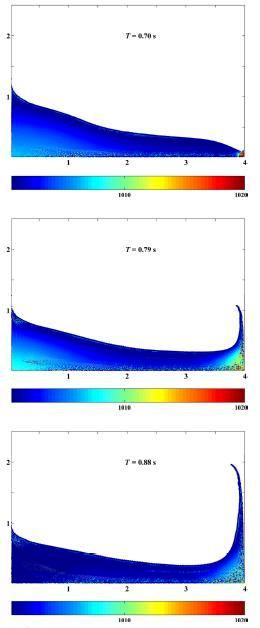
\includegraphics[scale=1]{figuras/sfiltro.jpg}
\caption{\textsc{Evolução da densidade sem a adoção de filtro de correção ao colidir com o muro}}
\vspace{-0.1cm}
\legend{FONTE: \citeonline{Crespo}}
\label{fig:sfiltro}
\end{figure}

\begin{figure}[H]
\centering
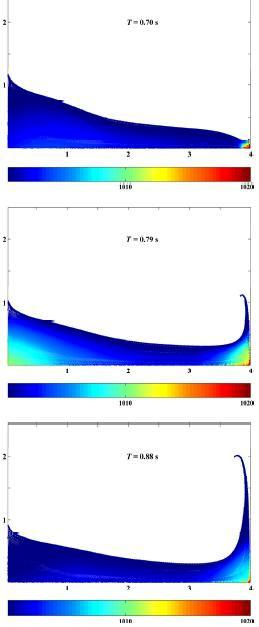
\includegraphics[scale=1]{figuras/cfiltroS.jpg}
\caption{\textsc{Evolução da densidade com a adoção de filtro de correção de Shepard ao colidir com o muro}}
\vspace{-0.1cm}
\legend{FONTE: \citeonline{Crespo}}
\label{fig:cfiltroS}
\end{figure}

\begin{figure}[H]
\centering
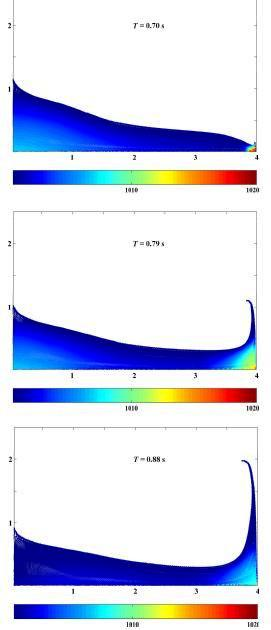
\includegraphics[scale=1]{figuras/cfiltroM.jpg}
\caption{\textsc{Evolução da densidade com a adoção de filtro de correção MLS ao colidir com o muro}}
\vspace{-0.1cm}
\legend{FONTE: \citeonline{Crespo}}
\label{fig:cfiltroM}
\end{figure}

Nesse trabalho, os autores ainda consideraram a simulação da ruptura de uma barragem para o caso de leito úmido, onde observaram o comportamento da frente de onda e, também, adotaram obstáculos a jusante da barragem, mas estes experimentos fogem do escopo desta dissertação.        
%---------------------------------------------------------------------------------------------
\section{MODELO UNIDIMENSIONAL} \label{Modelo1D}

Para a construção de um modelo unidimensional das equações de Euler conservativa, equações (\ref{massasis}) a (\ref{energiasis}),  foi utilizada uma adaptação do canal finito, Figura \ref{fig:tanque}, considerado em \citeonline{Crespo}.  

\begin{figure}[H]
	\centering
	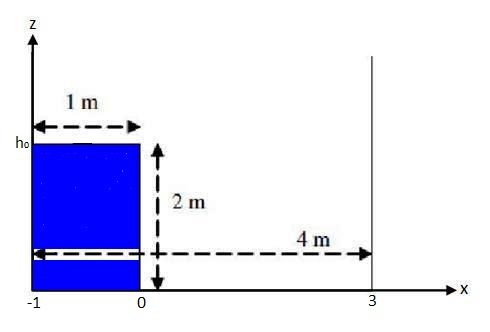
\includegraphics[scale=1]{figuras/tanque2.jpg}
	%\ includegraphics[width=.4\textwidth]{tanque2.jpg}
	\caption{\textsc{Canal finito simulando uma barragem hipotética}}
	\vspace{-0.1cm}
	\legend{FONTE: Adaptado de \citeonline{Crespo}}
	\label{tanque2}
\end{figure}

A modificação realizada, Figura \ref{tanque2}, define que a barragem está representada na origem do sistema cartesiano, $x=0$, separando dois níveis de leitos. À montante da barragem, $x<0$ , encontra-se o reservatório, com altura da coluna d'água igual a $h(x,0)=2 \ m$. À jusante, $x>0$, tem-se o leito seco, com altura da coluna d'água igual a $h(x,0)=0 \ m$. Essas diferenças nos leitos, conforme comentado na Seção \ref{visao}, formam níveis de transição nas propriedades físicas do escoamento e podem ser tratadas, matematicamente, como descontinuidades das quantidades físicas. Se essas descontinuidades não forem adequadamente modeladas irão conduzir a soluções espúrias.

Como passo inicial na formulação unidimensional, considera-se o escoamento incompressível, com a densidade $\rho = \text{constante}$ e o movimento da massa líquida ocorrendo somente na direção do eixo coordenado $x$. Dessa forma, as equações de conservação da massa e do momento nas equações de Euler, equações (\ref{massasis}) e (\ref{momentox}), serão escritas como
\begin{equation}\label{UIncomp}
u_x=0
\end{equation}
e 
\begin{equation} \label{momenIncomp}
\rho u_t + (\rho u^2 + P)_x = 0.
\end{equation}

Integrando a equação (\ref{UIncomp}) em função de $x$, resulta
\begin{equation} \label{Uf}
u(x,t)= f_1 (t),
\end{equation}
que independe de $x$.

Derivando a equação (\ref{Uf}) em função do tempo $t$ e substituindo o resultado encontrado na equação (\ref{momenIncomp}), obtêm-se
\begin{equation} \label{ContModif}
\rho f^{'}_{1}(t)+ P_x =0.
\end{equation}

Utilizando a hipótese de pressão hidrostática, equação (\ref{varpres}), e que a mesma é uma média da profundidade do canal, pode-se considerar que
\begin{equation}\label{PressaoMedia}
P = \rho g \frac{h(x,t)}{2}.
\end{equation} 

Substituindo a equação (\ref{PressaoMedia}) na equação (\ref{ContModif}), encontra-se
\begin{equation}\label{Derh}
\rho f^{'}_{1}(t) + \frac{\rho g}{2} h_x=0.
\end{equation}

Fazendo as devidas simplificações na equação (\ref{Derh}) e integrando o resultado em função de $x$, determina-se o perfil da superfície livre dado por
\begin{equation} \label{EQFINAL}
h(x,t) = \frac{-2f^{'}_{1}(t)x}{g} + f_2(t).
\end{equation}

Nos contornos do canal, Figura \ref{tanque2}, tem-se que $u(l,t)=0$ e $u(L,t) = 0$. Como $u(x,t)=f_1(t)$ independe de $x$, a equação (\ref{EQFINAL}) não terá solução. Isso mostra que a forma como foi construído o modelo unidimensional, usando as equações de Euler sob a hipótese de escoamento incompressível em canais finitos, não soluciona o problema da ruptura de barragens em questão.

%---------------------------------------------------------------------------------------------
\section{MODELO DE ÁGUAS RASAS} \label{ModeloAR}

O tratamento adotado para o modelo unidimensional, apresentado Seção \ref{Modelo1D}, mostrou não ser possível obter uma solução para o problema da ruptura de barragens utilizando a hipótese de escoamento incompressível em canais finitos. No entanto, em 1892, Ritter obteve uma solução para o problema considerando a hipótese de canais retangulares e infinitos \cite{Sakkas}. Essa solução foi determinada baseando-se no Método das Características \cite{Zenchuk} e \cite{Henderson}. Para tanto, seja
\begin{equation} \label{velonda}
c(x,t)= \sqrt{gh}
\end{equation}
a velocidade de propagação de uma onda, sendo $h \geq 0$ a profundidade total da superfície livre e $g$ a aceleração da gravidade. 

Multiplicando a equação de Águas Rasas (\ref{ARR2}) por $g$ e considerando, na equação (\ref{velonda}), que $c^2 = gh$, tem-se
\begin{equation} \label{ARR3}
(c^2)_t + (uc^2)_x = 0.
\end{equation} 

Derivando a  equação (\ref{ARR3}) e realizando as devidas simplificações, encontra-se
\begin{equation} \label{ARFim}
(2c)_t + u(2c)_x + cu_x = 0.
\end{equation}

Novamente, na  equação (\ref{velonda}), considerando que $h = {c^2}/{g}$ e substituindo na equação de Águas Rasas (\ref{AR2}), defini-se que
\begin{equation}\label{AR3}
u_t +uu_x + g \left( \frac{c^2}{g} \right)_x= 0.
\end{equation}

Sabendo que a derivada de $h = {c^2}/{g}$, em função de $x$, resulta em $h_x = 2cc_x /g$, a substituição desse resultado irá transformar a equação (\ref{AR3}) em
\begin{equation} \label{ARFim2}
u_t + uu_x + 2cc_x = 0.
\end{equation}

As equações (\ref{ARFim}) e (\ref{ARFim2}) formam o modelo de Águas Rasas unidimensional baseado na velocidade do escoamento $u$ e na velocidade de propagação da onda $c$. Somando e subtraindo essas equações resultará em um par de EDPs
\begin{equation}\label{SomAR}
\left[ \frac{ \partial}{ \partial t} + (u \pm c) \frac{ \partial}{ \partial x} \right](u \pm 2c) =0.
\end{equation}

Se, na equação (\ref{SomAR}) for considerado que
\begin{equation*}
\frac{d}{dt}(u \pm 2c) = 0,
\end{equation*}
então
\begin{equation*}
\frac{dx}{dt} = (u \pm c).
\end{equation*}

Desse resultado pode-se interpretar, por meio do Método das Características, que as inclinações das linhas características $ C^+ $ são definidas como
\begin{equation*}
\left. \frac{dx}{dt} \right|_{C^+} = (u + c)
\end{equation*}
e que, ao longo dessas linhas, $u + 2c = \text{constante}$.

De forma análoga, pode-se interpretar que as inclinações das linhas características $C^-$ são determinadas por
\begin{equation*}
\left. \frac{dx}{dt} \right|_{C^-} = (u - c)
\end{equation*}
e que, ao longo dessas linhas, $u - 2c = \text{constante}$.

As funções $u+2c$ e $u-2c$ são chamadas de invariantes de Riemann e se propagam, quer à montante $(-c)$ ou à jusante $(+c)$, em relação à velocidade do fluxo $u$.   

Uma classe especial de solução, chamada de onda simples, surge quando uma das invariantes de Riemann é sempre constante no domínio de interesse. Neste caso, se for considerada a propagação da uma onda, movendo-se para a direita, em águas estacionárias e com profundidade constante, $z=h$, então todas as linhas características $C^-$ surgirão da região não perturbada, conforme pode ser observado na Figura \ref{219B}. Além disso, como $u_0=0$ e $c_0 = \sqrt{gh_0}$, então a invariante de Riemann nessa região será
\begin{equation} \label{Equau}
u-2c=u_0 - 2c=-2c_0.
\end{equation}
Assim, $u-2c$ será sempre constante e, como $u+2c$ é constante nas linhas características $C^+$, irá implicar em $u$ e $c$ também constantes nas linhas $C^+$. 

\begin{figure}[H]
	\centering
	\includegraphics[scale=1]{figuras/219B.jpg}
	%\fbox{\includegraphics[width=.4\textwidth]{219B.jpg}}
	\caption{\textsc{As linhas características $C^+$ e $C^-$ para uma onda se propagando para direita numa região estacionária e de profundida constante}}
	\vspace{-0.1cm}
	\legend{FONTE: \citeonline{Johnson}}
	\label{219B}
\end{figure}

A forma de interpretar o caso da onda simples serve para compreender a estruturação da solução no caso da ruptura de barragens. Se for considerado que, para o tempo $t=0$, ocorre o colapso da estrutura localizada na origem do sistema $x=0$ e, nesse instante, 
\begin{equation*}
u= u_0 =0
\end{equation*}
e
\begin{equation*}
h(x, 0) = \left\{
	\begin{array}{rcl}
	h_0 \ ; \ x<0 &  & \\
	& & \\
	0 \ ; \ x>0 &  &, 
	\end{array} \right.
\end{equation*}
sendo $h_0>0$  constante, todas as características virão da região não perturbada $x<0$ e serão constantes, ou seja, 
\begin{equation*}
u+2c=2 \sqrt{gh_0}.
\end{equation*}

No momento em que se inicia o movimento da massa líquida irão surgir infinitas linhas características da origem $x=0$, todas com inclinações diferentes, pois cada $h$, $0 \leq h \leq h_0$, determina uma linha característica. Então, para tratar o fenômeno, há a necessidade de uma forma degenerada da solução característica.

Das linhas características $C^-$ tem-se que suas inclinações são
\begin{equation}\label{IncliC}
\frac{dx}{dt} = u-c,
\end{equation}
onde $u-2c$ é constante. Mas, $u+2c$ é constante e, assim, pode-se concluir que $u$, $c$, $u-c$ são constates e $C^-$ são linhas retas. Com isso, integrando a equação (\ref{IncliC}), em função de $t$, encontra-se
\begin{equation}\label{IntC}
x= (u-c)t,
\end{equation}
o que indica que todas estas linhas características $C^-$ irão passar pela origem do sistema $(0,0)$. Este comportamento das linhas características é chamado de leque de expansão, conforme mostra a Figura \ref{220B}.

\begin{figure}[H]
	\centering
	\includegraphics[scale=1]{figuras/220B.jpg}	%\fbox{\includegraphics[width=.4\textwidth]{220B.jpg}}
	\caption{\textsc{As linha características $C^+$ e $C^-$ para o problema da ruptura de barragens}}
	\vspace{-0.1cm}
	\legend{FONTE: \citeonline{Johnson}}
	\label{220B}
\end{figure}

Da condição inicial em que $u(0)=0$, tem-se
\begin{equation} \label{CDini}
u+2c=2 \sqrt{gh_0}= 2c_0,
\end{equation}
ou seja,
\begin{equation} \label{condi1}
u= 2c_0 -2c.
\end{equation}

Da hipótese de todas as linhas características $C^-$ passarem pela origem do sistema, equação (\ref{IntC}), pode-se obter
\begin{equation} \label{caracC}
\frac{x}{t} = u-c
\end{equation}
que, ao substituir $u$ pela equação (\ref{condi1}), transforma-se na equação
\begin{equation} \label{soma}
\frac{x}{t} = 2c_0 - 3c = 2c_0 - 3 \sqrt{gh},
\end{equation}
ou seja,
\begin{equation*}
\sqrt{gh} = \frac{1}{3} \left( 2c_0 - \frac{x}{t} \right)
\end{equation*}
determinando que a profundida da superfície livre, após o início do escoamento, será obtida por
\begin{equation} \label{solzAR}
h(x,t)= \frac{1}{9} \left[2 \sqrt{gh_0} - \frac{x}{t} \right]^2.
\end{equation}

Se, na equação (\ref{CDini}), for definido que
\begin{equation*}
c = c_0 - \frac{u}{2},
\end{equation*}
então a equação (\ref{IntC}) pode ser escrita na forma
\begin{equation*}
\frac{x}{t} = u - c_0 + \frac{u}{2},
\end{equation*}
ou seja,
\begin{equation*}
\frac{3u}{2} = \frac{x}{t} + c_0,
\end{equation*}
determinando que a velocidade do escoamento será obtida por
\begin{equation} \label{soluAR}
u(x,t)= \frac{2}{3} \left[ \frac{x}{t} + \sqrt{gh_0} \right].
\end{equation}

Assim, considerando a região localizada entre $h=h_0$ até $h=0$, as equações (\ref{solzAR}) e (\ref{soluAR}) irão descrever o perfil da superfície livre (alturas e velocidades do escoamento), desde que $-t \sqrt{gh_0} \leq x \leq 2t \sqrt{gh_0}$ para $t>0$ e que, pela equação (\ref{soma}), $x/t=u- \sqrt{gh} =2 \sqrt{gh_0} - 3 \sqrt{gh}$.

A equação (\ref{solzAR}) irá formar, após o início do movimento da massa líquida, uma parábola entre o ponto à montante, onde a influência do escoamento ainda não é sentida $(x=-c_0 t)$, e a frente de onda, ponto mais à jusante $(x=2c_0 t)$. Na origem do sistema, onde estava localizada a barragem, a altura da coluna d'água irá atingir um valor constante $h(0,t)= 4h_0 / 9$ para $t>0$. Quando $t\longrightarrow \infty$, a profundidade irá se aproximar deste mesmo valor constante em todos os lugares. A Figura \ref{ondalonga} esquematiza o perfil da superfície livre após a ruptura da barragem.


\begin{figure}[H]
	\centering
	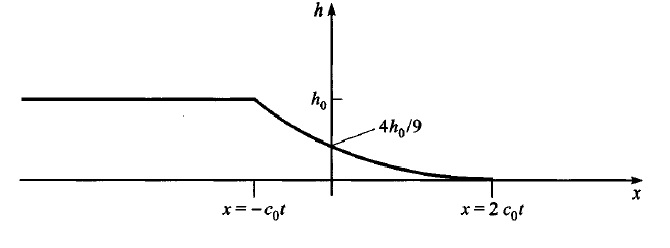
\includegraphics[scale=1]{figuras/ondalonga.jpg}	%\fbox{\includegraphics[width=.4\textwidth]{220B.jpg}}
	\caption{\textsc{O perfil da superfície livre para o tempo $t$ após a ruptura de barragens}}
	\vspace{-0.1cm}
	\legend{FONTE: \citeonline{Johnson}}
	\label{ondalonga}
\end{figure}
     



%------------------------------------------------------------------------------------------------------------------------------------------------------
\section{O CÓDIGO PySPH} \label{py}

Dentre os inúmeros códigos desenvolvidos para o método SPH destaca-se o PySPH, por ser um código aberto, com processamento em paralelo e implementado em Python, que é uma linguagem de alto nível, orientada a objeto, com programação interpretada e de fácil aprendizagem.

O PySPH foi apresentado no trabalho de \citeonline{Ramachandran2010} que desenvolveram este código com o intuito de suprir a comunidade científica com um código de fonte aberta e com repositório acessível ao público, detalhes estes que não são encontrados em outras implementações, conforme destacam os autores. 

O Python, por ser uma linguagem interpretada, torna o processamento lento. No entanto, para contornar esta dificuldade no PySPH, toda a performance crítica do processamento foi desenvolvida em Cython, que é uma linguagem escrita em C com extensões para Python, ou seja, ao compilar um módulo em Cython este é compilado em extensões C que podem ser importados para Python, agilizando todo o processo. 

De forma geral, para realizar as simulações, o PySPH utiliza poucos objetos chaves, tais como \textit{Solver}, que controla outras funções como o integrador, ou as \textit{Entities}, que são coleções de partículas que podem representar classes de entidades físicas, como fluidos ou sólidos. Uma visão simplificada deste processo pode ser visto na Figura \ref{fig:diagrama} onde estão delineadas as principais fases. Cada uma destas fases, bem como uma visão mais detalhada sobre a arquitetura do código, pode ser encontrada no repositório desenvolvidos pelos autores \citeonline{PySPH}.

\begin{figure}[H]
\centering
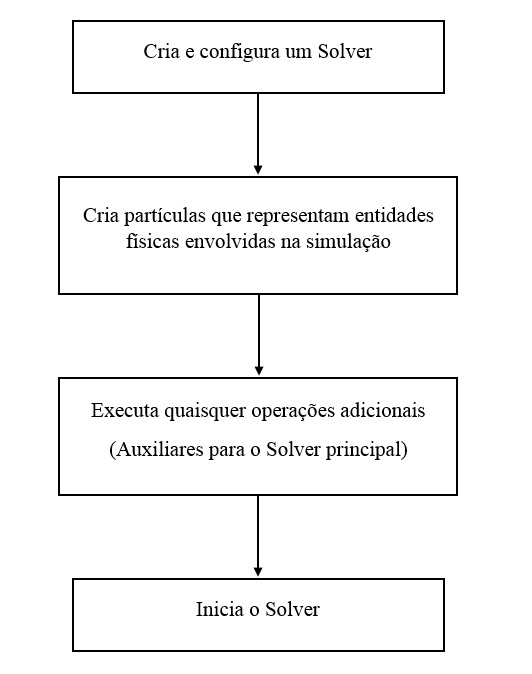
\includegraphics[scale=0.8]{figuras/diagrama.jpg}
\caption{\textsc{Esboço das tarefas executadas numa simulação em PySPH}}
\vspace{-0.1cm}
\legend{FONTE: Adaptado de \citeonline{Ramachandran2010}}
\label{fig:diagrama}
\end{figure}

A eficiência do código é comprovada por meio de alguns exemplos, entre eles está a ruptura de uma barragem hipotética seguindo o trabalho de \citeonline{Crespo}. Para tanto, consideraram a Figura \ref{fig:tanque} como representando a barragem. Como parâmetros utilizaram as condições de fronteira dinâmica e formaram um \textit{grid} de mesmo espaçamento nas direções dos eixos coordenados $x$ e $y$ de tamanho $dx=dy=0,03 \ m$. Com isso, utilizaram $4.556$ partículas representando o fluido e $671$ partículas representado as fronteiras. Utilizaram a suavização do núcleo igual a $h=0,039 \ m$ resultando em um raio de atuação do núcleo igual a $h/dx=1,3 \ m$, o que utiliza, aproximadamente, $21$ vizinhos para cada partícula por passo adotado, conforme comenta \citeonline{Liu2003}. Como tamanho de passo consideraram $dt=10^{-4}s$, com tempo total de simulação igual a $tf=1s$.

Além dos parâmetros acima destacados, \citeonline{Ramachandran2010} adotaram também a densidade da água como $\rho=1000 \ kg/m^{3}$, velocidade do som como $co=10 \times \sqrt{2 \times 9,81 \times 2} \ m/s$, $\alpha=0,5$ como fator de correção XSPH, $\gamma=7,0$ utilizada como uma constante na equação de estado e $B=co^2 \times \rho/ \gamma$ como valor para o termo relacionado às flutuações de densidade do fluido.

Das equações utilizadas em SPH para modelar a ruptura de barragens, como a equação da continuidade (\ref{Cont_SPH}) e a equação do momento (\ref{Mov_SPH}), destaca-se a equação de estado
\begin{equation} \label{estado}
P=B \left[\left(\frac{\rho}{\rho_0}\right)^{\gamma}-1\right],
\end{equation} 
que é a equação de Tait que descreve uma relação entre a pressão e a densidade \cite{Monaghan1994}. Conforme destacam \citeonline{Crespo}, a constante $\gamma$ pode variar entre $1$ e $7$, sendo que $\gamma=7$ é normalmente usada para aplicações oceânicas. Ainda, segundo esses autores, a utilização dessa equação evita o cálculo da pressão da equação de Poisson, o que reduz o esforço computacional.

Para formação dos núcleos, nesta simulação, os autores utilizaram a função Spline de quinto grau, já que este tipo de função tem um comportamento próximo de uma função gaussiana, mas não melhor que a Spline cúbica, conforme pode ser observado na Figura \ref{fig:nucleos}.

Alguns resultados para comprovar a eficiência do código PySPH, em diferentes tempos de simulação, foram obtidos para o problema modelo e serão apresentados  e discutidos na Seção \ref{REPy}. 
%obtidos podem ser observados nas figuras (\ref{fig:pysph01s}) - (\ref{fig:pysphfim}).


      

%------------------------------------------------------------------------------------------------------------------------------------------------------
\section{PROPOSTA DA PESQUISA} \label{proposta}

Como objetivo principal desta dissertação, foi proposto a modelagem computacional da ruptura de uma barragem hipotética, cujo movimento da massa líquida era governado pelas equações de Euler. Para atingir esse objetivo as equações seriam discretizadas por meio do MDFE, em associação com o esquema difusivo de Lax-Friedrichs. No entanto, conforme destaca \citeonline{Stansby}, os estágios iniciais do movimento da massa líquida são os mais importantes em toda simulação, pois são nesses instantes em que se iniciam a formação das ondas de choques ou rarefação e métodos como o MDFE, associado a esquemas difusivos, não têm um comportamento adequado para o tratamento dessas descontinuidades, já que são considerados métodos de primeira ordem \cite{Crossley}.

Para manter o objetivo do trabalho, foram obtidas as equações de Águas Rasas (\ref{ARR2}) e (\ref{AR2}) considerando o escoamento levemente compressível nas equações de Euler. Isso permitiu definir, com o auxílio do Método das Características, uma solução analítica para o perfil do escoamento nos estágios iniciais do movimento da massa líquida, equações (\ref{solzAR}) e (\ref{soluAR}).

A formulação desenvolvida nas equações (\ref{solzAR}) e (\ref{soluAR}) baseou-se na hipótese do escoamento ocorrer em canais infinitos. No entanto, essa hipótese não condiz com o modelo hipotético adotado mostrado na Figura \ref{tanque2}. Assim, as equações (\ref{solzAR}) e (\ref{soluAR}) foram adequadas para o modelo em questão, ou seja, para o caso de um canal finito. Dessa forma, considerando $h_0=2 \ m$ o perfil inicial da coluna d'água, $l=1 \ m$ a lateral esquerda do tanque e $L=4 \ m$ a lateral direita, as soluções analíticas do perfil da superfície livre $h(x,t)$ e da velocidade média do escoamento $u(x,t)$ passaram a ser determinadas por 
\begin{equation} \label{solzMod}
	h(x,t)= \frac{1}{9g} \left[2 \sqrt{gh_0} - \frac{l-x}{t} \right]^2
\end{equation}
e
\begin{equation} \label{soluMod}
	u(x,t)=2 \left[ \sqrt{gh_0} - \sqrt{gh} \right],
\end{equation}
desde que $g=9,8m/s^2$ seja a aceleração de gravidade, $l-t \sqrt{gh_0} \leq x \leq l+2t \sqrt{gh_0}$ e que $0 \leq t \leq min \left\{l/ \sqrt{gh_0}\ ,\ (L-l)/2 \sqrt{gh_0} \right\}$.

Porém, se $x<l-t \sqrt{gh_0}$, tem-se
\begin{equation} \label{solzMod1}
	h(x,t)=h_0
\end{equation}
e
\begin{equation} \label{soluMod1}
	u(x,t)=0.
\end{equation}

Para o caso em que $x>l+2t \sqrt{gh_0}$, a solução será dada por
\begin{equation} \label{solzMod2}
	h(x,t)=0
\end{equation}
e
\begin{equation} \label{soluMod2}
	u(x,t)=0.
\end{equation}

Essa solução analítica, conforme construída acima, é capaz de tratar os estágios iniciais do movimento da massa líquida, já que evita a formação de ondas de choque ou rarefação, momento crítico na simulação. Esse processo torna possível a adoção do esquema numérico proposto anteriormente, pois quando $x>l+2t \sqrt{gh_0}$ e  $t \longrightarrow \infty$ a profundidade da superfície livre atinge um valor constante, ou seja, tende a se estabilizar. Assim, a partir desse ponto, o uso do MDFE torna-se adequado e passa a utilizar, como condições iniciais, os valores de $h(x,t)$ e $u(x,t)$ obtidos analiticamente.

   
%------------------------------------------------------------------------------------------------------------------------------------------------------
\section{A GERAÇÃO DA MALHA} \label{malha}

O modelo computacional desenvolvido utilizou uma forma híbrida para resolver o problema da ruptura de barragens, já que adotou uma solução analítica, para os instantes iniciais do escoamento, juntamente com uma solução numérica para os demais momentos da simulação, o que evitou a formação das ondas de choque e/ou rarefação e tornou a solução final possível sem conduzir para resultados espúrios.

Para construção da parte analítica do modelo fez-se uso das soluções obtidas na Seção \ref{ModeloAR} com as modificações realizadas na Seção \ref{proposta}. Já para a parte numérica, o modelo utilizou, como fundamentação, as equações de Águas Rasas (\ref{ARR2}) e (\ref{AR2}), discretizadas por meio do MDFE (\ref{explícito}), resultando em
\begin{equation} \label{A}
\frac{h^{n+1}_{i}-h^{n}_{i}}{\Delta t}= - \left[h^{n}_{i} \left( \frac{u^{n}_{i+1}-u^{n}_{i-1}}{2 \Delta x} \right) + u^{n}_{i} \left( \frac{h^{n}_{i+1}-h^{n}_{i-1}}{2 \Delta h} \right) \right]
\end{equation}   
e
\begin{equation} \label{B}
\frac{u^{n+1}_{i}-u^{n}_{i}}{\Delta t}= - \left[u^{n}_{i} \left( \frac{u^{n}_{i+1}-u^{n}_{i-1}}{2 \Delta x} \right) + g \left( \frac{h^{n}_{i+1}-h^{n}_{i-1}}{2 \Delta h} \right) \right].
\end{equation}

Explicitando os termos para o tempo $t=n+1$, as equações discretas (\ref{A}) e (\ref{B}) tornaram-se iguais a
\begin{equation} \label{C}
h^{n+1}_{i} =  h^{n}_{i} - \frac{\Delta t}{2} \left[h^{n}_{i} \left( \frac{u^{n}_{i+1}-u^{n}_{i-1}}{ \Delta x} \right) + u^{n}_{i} \left( \frac{h^{n}_{i+1}-h^{n}_{i-1}}{ \Delta h} \right) \right]
\end{equation}
e
\begin{equation} \label{D}
u^{n+1}_{i} = u^{n}_{i} - \frac{\Delta t}{2} \left[u^{n}_{i} \left( \frac{u^{n}_{i+1}-u^{n}_{i-1}}{ \Delta x} \right) + g \left( \frac{h^{n}_{i+1}-h^{n}_{i-1}}{ \Delta h} \right) \right].
\end{equation}

Para simplificar o modelo, considerou-se uma discretização constante, tanto para altura da superfície livre $h$ como para direção da velocidade do escoamento $x$. Com isso, pôde-se adotar $ \Delta h = \Delta x = \Delta$ e, dessa forma, as equações (\ref{C}) e (\ref{D}) passaram a ser escritas como
\begin{equation} \label{E}
h^{n+1}_{i} =  h^{n}_{i} - \alpha \left[h^{n}_{i} \left( u^{n}_{i+1}-u^{n}_{i-1} \right) + u^{n}_{i} \left( h^{n}_{i+1}-h^{n}_{i-1} \right) \right]
\end{equation}
e
\begin{equation} \label{F}
u^{n+1}_{i} = u^{n}_{i} - \alpha \left[u^{n}_{i} \left( u^{n}_{i+1}-u^{n}_{i-1} \right) + g \left( h^{n}_{i+1}-h^{n}_{i-1} \right) \right]
\end{equation}
onde $ \alpha = { \Delta t}/{2 \Delta}$.

A aplicação do esquema difusivo de Lax-Friedrichs (\ref{ELF}) nas equações (\ref{E}) e (\ref{F}) resultou no modelo final para simulação numérica proposta, ou seja, a suavização das equações resultou em
\begin{equation} \label{G}
	\small{ h^{n+1}_{i} =0.5 \left( h^{n}_{i+1}+h^{n}_{i-1} \right)  - \alpha \left[ 0.5 \left( h^{n}_{i+1}+h^{n}_{i-1} \right) \left( u^{n}_{i+1}-u^{n}_{i-1} \right)  + 0.5 \left( u^{n}_{i+1}+u^{n}_{i-1} \right) \left( h^{n}_{i+1}-h^{n}_{i-1} \right) \right] }
\end{equation}
e
\begin{equation} \label{H}
	u^{n+1}_{i} =0.5 \left( u^{n}_{i+1}+u^{n}_{i-1} \right) - \alpha \left[ 0.5 \left( u^{n}_{i+1}+u^{n}_{i-1} \right) \left( u^{n}_{i+1}-u^{n}_{i-1} \right) + g \left( h^{n}_{i+1}-h^{n}_{i-1} \right) \right]
\end{equation}
com condições de contorno $u(0,t)=0$, $u(L,t)=0$ e condições iniciais determinadas pelas soluções analíticas da Seção \ref{ModeloAR}.

Para garantir a estabilidade do modelo, a condição (\ref{CFL}) define que
\begin{equation}
\Delta t = Co \times \Delta.
\end{equation}
Como o tanque que simula a barragem hipotética possui um comprimento de $L=4 \ m$ optou-se por considerar uma discretização total de $400$ passos na direção do escoamento, o que proporcionou um incremento infinitesimal, na direção $x$,  igual a $ \Delta = 0,01 \ m$. Assim, adotando como condição de estabilidade $Co=0,01$, obteve-se o incremento infinitesimal para o avanço no tempo igual a
\begin{equation}
\Delta t = 0,01 \times 0,01 = 0,0001s,
\end{equation}
proporcionando uma quantidade razoável de amostras para compor as médias da elevação do perfil da coluna d'água e da velocidade do escoamento, capazes de representar alguns fenômenos que surgem no problema físico. 

      







%-------------------------------------------------------------------------------------------------------------------------------------------------------

%\section{VARIAÇÃO DOS PARÂMETROS} \label{parametros}



\chapter{RESULTADOS}
%Título Capítulo 6
Alguns experimentos para diferentes tempos de simulação foram realizados, tanto no modelo de configuração euleriana proposto nessa dissertação, como no código lagrageano PySPH utilizado como referência. Os resultados mais significativos encontrados, utilizando o modelo de híbrido, são analisados na Seção \ref{Hibri}, enquanto aqueles obtidos por meio do código PySPH são apresentados na Seção \ref{REPy}.  Um comparativo entre os resultados encontrados nesses dois método é discutido na Seção \ref{Comparacao}.  


\section{ANÁLISE DOS RESULTADOS OBTIDOS} \label{Hibri}

 A estratégia utilizada para a obtenção dos resultados, utilizando o código desenvolvido nesse trabalho, consistiu em determinar valores médios para as velocidades e as alturas atingidas pelo perfil da coluna d'água. Cada intervalo de tempo adotado foi incrementado, inicialmente, em $t= 0,05s$ com o intuito de compor os valores médios. Essa estratégia tornou possível um bom tratamento e análise dos resultados, uma vez que eliminou valores que prejudicavam a representação gráfica. Além disso, o comprimento do tanque foi discretizado em intervalos de $x=0,2 \ m$ o que permitiu a visualização dos perfis nos diversos ponto do escoamento e em todos os tempos de simulação, ou seja, até atingir o estado de regime permanente do escoamento.
 
 O primeiro ponto adotado para visualizar o escoamento foi $x= 0,2 \ m$, com tempo total de simulação de aproximadamente $t = 7,5s$, momento em que as velocidades e as alturas iniciam um estado de regime permanente, Figura \ref{perfil2s}.
 
 Nota-se nessa figura o aumento das velocidades e a diminuição das alturas no exato momento em que se inicia o movimento da coluna d'água, o que representou, com boa fidelidade, o fenômeno físico. Logo após, as velocidades, bem como as alturas, tendem a se estabilizarem indicando que a coluna d'água ainda está percorrendo a extensão do canal. Em seguida, há uma acentuada queda nas velocidades, acompanhada por uma elevação no perfil das alturas, o que confere com o momento em que o fluido colide com o muro localizado no lado direito do canal, $L=4 \ m$, formando o \textit{sloshing}, fenômeno esse que pode ser visto em detalhes no trabalho de \citeonline{Carbajal}. Após isso, tanto as velocidades como as alturas tendem a oscilar, devido às colisões, em menores escalas, com os muros laterais, até atingirem o estado, aparentemente, estacionário. 
 
 \begin{figure}[H]
 	\centering
 	% 	\fbox{\includegraphics[scale=.6]{perfil2s.jpg}}
 	\includegraphics[scale=1]{figuras/perfil2s.jpg}
 	\caption{\textsc{Perfil da velocidade média $u$ e a altura da coluna d'água $h$ para o ponto $x=0,2 \ m$}}
 	\vspace{-0.1cm}
 	\legend{FONTE: Programa do autor usando as equações de Águas Rasas}
 	\label{perfil2s}
 \end{figure}
 
 Uma análise semelhante ao que foi feito anteriormente pode ser realizada na Figura \ref{perfil04s}. No entanto, percebe-se que as velocidades são maiores, já que o ponto adotado para compor as médias é agora de $x= 0,4 \ m$, ou seja, valores diferentes compõem as médias. Assim, é possível notar os momentos de colisão com os muros e a formação do \textit{sloshing} numa posição diferente do tanque.
 
 Comparando a Figura \ref{perfil2s} com a Figura \ref{perfil04s} observa-se que as velocidades têm médias iniciais nulas, o mesmo ocorrendo com as alturas da coluna d'água que permanecem com  $h=2 \ m$. Esse fato ocorre pois, nos primeiros instantes do escoamento, tanto $u$ como $h$ são determinados pelas equações (\ref{solzMod1}) e (\ref{soluMod1}). 
 
 \begin{figure}[H]
 	\centering
 	% 	\fbox{\includegraphics[scale=.6]{perfil04s.jpg}}
 	\includegraphics[scale=1]{figuras/perfil04s.jpg}
 	\caption{\textsc{Perfil da velocidade média $u$ e a altura da coluna d'água $h$ para o ponto $x=0,4 \ m$} }
 	\vspace{-0.1cm}
 	\legend{FONTE: Programa do autor usando as equações de Águas Rasas}
 	\label{perfil04s}
 \end{figure}
 
 Considerando as médias em um ponto mais distante da barragem,  $x= 1,0 \ m$, Figura \ref{perfil0s}, alguns fenômenos físicos no início do movimento deixam de ser capturados. Observa-se que as velocidades médias são maiores do que as anteriores, aproximadamente $u=3 \ m/s$, já neste ponto a massa líquida está percorrendo o tanque ainda sob ação da queda. O mesmo ocorre com as alturas, onde não estão mais claros os perfis iniciais da barragem antes de sua ruptura. Nota-se também, que há pouca captura dos fenômenos formados no momento em que o fluido colide com os muros.
 
 \begin{figure}[H]
 	\centering
 	% 	\fbox{\includegraphics[scale=.6]{perfil10s.jpg}}
 	\includegraphics[scale=1]{figuras/perfil10s.jpg}
 	\caption{\textsc{Perfil da velocidade média $u$ e a altura da coluna d'água $h$ para o ponto $x=1,0 \ m$}}
 	\vspace{-0.1cm}
 	\legend{FONTE: Programa do autor usando as equações de Águas Rasas}
 	\label{perfil0s}
 \end{figure}
 
 Ainda dentro dessa linha de raciocínio, para Figura \ref{perfil4s}, localizada no ponto $x= 1,4 \ m$, observa-se que a velocidade média atinge o seu máximo, $u=8,5 \ m/s$, quando a altura do fluido ainda é próxima de zero. Isso ocorre devido à posição em que o ponto se encontra, já que nesse caso as médias são calculadas por meio das equações (\ref{solzMod}) e (\ref{soluMod}).
 
 \begin{figure}[H]
 	\centering
 	% 	\fbox{\includegraphics[scale=.6]{perfil14s.jpg}}
 	\includegraphics[scale=1]{figuras/perfil14s.jpg}
 	\caption{\textsc{Perfil da velocidade média $u$ e a altura da coluna d'água $h$ para o ponto $x=1,4 \ m$}}
 	\vspace{-0.1cm}
 	\legend{FONTE: Programa do autor usando as equações de Águas Rasas}
 	\label{perfil4s}
 \end{figure}
 
 No caso das Figuras \ref{perfi20s} e \ref{perfi30s} os pontos estão localizados em $x= 2,0 \ m$ e $x= 3,0 \ m$, respectivamente. Essas localizações mostraram-se pouco eficientes na captura dos fenômenos formados, já encontram-se afastadas tanto da barragem como do muro direito. No entanto, serviram para verificar a funcionalidade do código implementado, pois as médias, nos instantes iniciais do escoamento, foram calculadas por intermédio das equações (\ref{solzMod2}) e (\ref{soluMod2}).
 
 \begin{figure}[H]
 	\centering
 	% 	\fbox{\includegraphics[scale=.6]{perfil20s.jpg}}
 	\includegraphics[scale=1]{figuras/perfil20s.jpg}
 	\caption{\textsc{Perfil da velocidade média $u$ e a altura da coluna d'água $h$ para o ponto $x=2,0 \ m$}}
 	\vspace{-0.1cm}
 	\legend{FONTE: Programa do autor usando as equações de Águas Rasas}
 	\label{perfi20s}
 \end{figure}
 
 \begin{figure}[H]
 	\centering
 	% 	\fbox{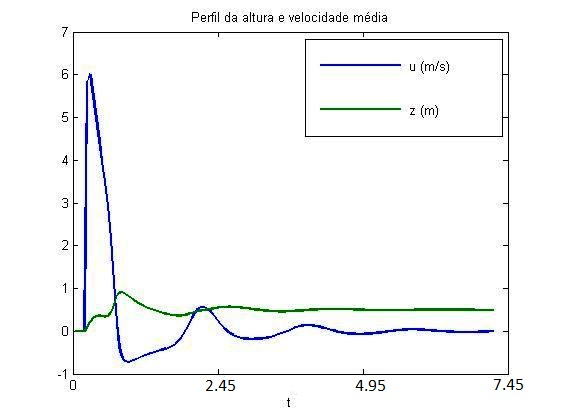
\includegraphics[scale=.6]{perfil30s.jpg}}
 	\includegraphics[scale=1]{figuras/perfil30s.jpg}
 	\caption{\textsc{Perfil da velocidade média $u$ e a altura da coluna d'água $h$ para o ponto $x=3,0 \ m$}}
 	\vspace{-0.1cm}
 	\legend{FONTE: Programa do autor usando as equações de Águas Rasas}
 	\label{perfi30s}
 \end{figure}
 
 Outra forma de análise que pode ser realizada no experimento é verificar o comportamento da massa líquida em certos tempos de simulação, já que os resultados determinados pelo modelo, conforme comentado anteriormente, também foram incrementados a cada $t=0,05s$. Assim, se for considerado o perfil de altura da coluna d'água, pode-se analisar seu comportamento durante o percurso dentro do tanque, como mostra a Figura \ref{Alt01s} que simula o escoamento no início do movimento $t=0,05s$.
 
 \begin{figure}[H]
 	\centering
 	% 	\fbox{\includegraphics[scale=.6]{perfil30s.jpg}}
 	\includegraphics[scale=1]{figuras/Alt01s.jpg}
 	\caption{\textsc{Perfil de altura da coluna d'água $h$ para o tempo $t=0,05s$}}
 	\vspace{-0.1cm}
 	\legend{FONTE: Programa do autor usando as equações de Águas Rasas}
 	\label{Alt01s}
 \end{figure}
 Nota-se nessa figura que o perfil do reservatório está bem definido $h=2 \ m$ e logo após a posição $x=0,6 \ m$ inicia-se o escoamento, elevando a altura da coluna d'água formando a frente de onda.
 
 Na Figura \ref{alt1s} o tempo de simulação é de $t=0,1s$. Nesse instante de tempo a coluna d'água atinge um ponto mais distante da barragem, $x=1,6 \ m$ e já há uma  diminuição na altura do reservatório.
 \begin{figure}[H]
 	\centering
 	% 	\fbox{\includegraphics[scale=.6]{perfil30s.jpg}}
 	\includegraphics[scale=1]{figuras/alt1s.jpg}
 	\caption{\textsc{Perfil de altura da coluna d'água $h$ para o tempo $t=0,1s$}}
 	\vspace{-0.1cm}
 	\legend{FONTE: Programa do autor usando as equações de Águas Rasas}
 	\label{alt1s}
 \end{figure}
 
 Percebe-se na Figura \ref{Alt2s} que o perfil da superfície livre, no tempo $t=0,2s$, já se aproxima do resultado mostrado na Figura \ref{ondalonga} indicando que profundidade está se tornado constante em toda distância do tanque.
 \begin{figure}[H]
 	\centering
 	% 	\fbox{\includegraphics[scale=.6]{perfil30s.jpg}}
 	\includegraphics[scale=1]{figuras/Alt2s.jpg}
 	\caption{\textsc{Perfil de altura da coluna d'água $h$ para o tempo $t=0,2s$}}
 	\vspace{-0.1cm}
 	\legend{FONTE: Programa do autor usando as equações de Águas Rasas}
 	\label{Alt2s}
 \end{figure}
 
 A formação do \textit{sloshing} pode ser notado na Figura \ref{Alt35s} quando a coluna d'água atinge o muro no lado direito do tanque logo após o tempo $t=0,35s$.
 \begin{figure}[H]
 	\centering
 	% 	\fbox{\includegraphics[scale=.6]{perfil30s.jpg}}
 	\includegraphics[scale=1]{figuras/Alt35s.jpg}
 	\caption{\textsc{Perfil de altura da coluna d'água $h$ e a formação do \textit{sloshing} no tempo $t=0,35s$}}
 	\vspace{-0.1cm}
 	\legend{FONTE: Programa do autor usando as equações de Águas Rasas}
 	\label{Alt35s}
 \end{figure}
 
 Após a formação do \textit{sloshing} a frente de onda atinge uma altura próxima de $h=1,2 \ m$ e começa a retornar seu percurso até atingir o muro lateral esquerdo, como pode ser observado na Figura \ref{Alt75s}. Logo após, a altura da frente de onda diminui, $h=0,6 \ m$ se aproximando mais ainda do muro esquerdo, Figura \ref{Alt120s}.
  
 \begin{figure}[H]
 	\centering
 	% 	\fbox{\includegraphics[scale=.6]{perfil30s.jpg}}
 	\includegraphics[scale=1]{figuras/Alt75s.jpg}
 	\caption{\textsc{Perfil de altura da coluna d'água $h$ para o tempo $t=0,75s$}}
 	\legend{FONTE: Programa do autor usando as equações de Águas Rasas}
 	\label{Alt75s}
 \end{figure}
 
  \begin{figure}[H]
  	\centering
  	% 	\fbox{\includegraphics[scale=.6]{perfil30s.jpg}}
  	\includegraphics[scale=1]{figuras/Alt120s.jpg}
  	\caption{\textsc{Perfil de altura da coluna d'água $h$ para o tempo $t=1,2s$}}
  	\vspace{-0.1cm}
  	\legend{FONTE: Programa do autor usando as equações de Águas Rasas}
  	\label{Alt120s}
  \end{figure}
  
  Depois de colidir com o muro no lado esquerdo do tanque a frente de onda retorna seu movimento para direção do escoamento até colidir novamente com o muro do lado direito. Esse movimento se repete até que as velocidade se anulem e a profundidade se torne constante. A Figura \ref{Alt350s} mostra a altura da frente de onda oscilando entre $h=0,48 \ m$ e $h=0,52 \ m$ no tempo de simulação $t=3,5s$.
  \begin{figure}[H]
  	\centering
  	% 	\fbox{\includegraphics[scale=.6]{perfil30s.jpg}}
  	\includegraphics[scale=1]{figuras/Alt350s.jpg}
  	\caption{\textsc{Oscilação do frente de onda no tempo $t=3,5s$}}
  	\legend{FONTE: Programa do autor usando as equações de Águas Rasas}
  	\label{Alt350s}
  \end{figure}   	      
 
   
%------------------------------------------------------------------------------------------------------------------------------------------------------
\section{ANÁLISE DOS RESULTADOS OBTIDOS NO PySPH} \label{REPy}

Devido à complexidade dos cálculos que envolvem o método SPH na formação dos núcleos e suas vizinhanças, na construção das fronteiras, sejam elas fantasmas ou dinâmicas, entre outros, exige uma capacidade de processamento de máquina considerável. A utilização do código PySPH não modificou essa realidade, mesmo os cálculos mais complexos sendo realizados em Cython. O tempo de processamento gasto para simular o exemplo citado na Seção \ref{py} foi de aproximadamente $30$ minutos em um computador pessoal com velocidade de processamento de $1.6 \  GHz$ e $2 \ GB$ de memória RAM. Esse tempo sobe para mais de $10h$ quando a suavização do núcleo diminui para $h=0,0156 \ m$, resultando em $28.056$ partículas para representar o fluido e $1.669$ partículas para formar as fronteiras.

Apesar do tempo gasto na simulação ser alto, o código foi capaz de representar o fenômeno da ruptura de barragens, uma vez que sua eficiência já havia sido comprovada no trabalho de \citeonline{Ramachandran2010}. No entanto, alguns parâmetros como tempo de simulação, tamanho do núcleo e tipo de fronteira foram alterados nesse experimento.

O primeiro resultado obtido foi para o início do escoamento $t=0,01s$, onde os valor da densidade da massa líquida já começam a sofrer alterações, como pode ser visto na Figura \ref{fig:pysph01s}.   

\begin{figure}[H]
	\centering
	\includegraphics[scale=0.5]{figuras/pysph01s.png}
	\caption{\textsc{Mudanças nos valores da densidade no início da simulação $t=0,01s$}}
	\vspace{-0.1cm}
	\legend{FONTE: Simulação do autor utilizando o código PySPH}
	\label{fig:pysph01s}
\end{figure}

Para o tempo $t=0,1s$ a massa líquida já começa a se deslocar, formando a frente de onda. No entanto, divido a ação das partículas que compõem o fundo do canal, há uma elevação nesse ponto, Figura \ref{fig:pysph1s}. Como alternativa para o problema, a solução poderia ser refinado considerando-se um maior número de partículas compondo o fluido, mas o esforço computacional seria maior. 

\begin{figure}[H]
	\centering
	\includegraphics[scale=0.5]{figuras/pysph1s.png}
	\caption{\textsc{Alteração nos valores da densidade próximo ao leito $t=0,1s$}}
	\vspace{-0.1cm}
	\legend{FONTE: Simulação do autor utilizando o código PySPH}
	\label{fig:pysph1s}
\end{figure}

Na Figura \ref{fig:pysph2s} a ação das partículas fantasmas se torna mais evidente. Além disso, nota-se que o perfil da superfície livre não está escoando e sim descendo, com algumas partículas ainda presas na lateral esquerda do tanque. 

\begin{figure}[H]
	\centering
	\includegraphics[scale=0.5]{figuras/pysph2s.png}
	\caption{\textsc{Evolução da coluna d'água sobre o leito $t=0,2s$}}
	\vspace{-0.1cm}
	\legend{FONTE: Simulação do autor utilizando o código PySPH}
	\label{fig:pysph2s}
\end{figure}

Os efeitos das fronteira continuam agindo sobre o escoamento, Figura \ref{fig:pysph4s}, afastando a frente de onda do fundo do tanque. Esse efeito é justamente a forma como deve atuar as fronteiras, ou seja, repelir evitando que as partículas do fluido passem para fora do tanque. No entanto, esse efeito deve ser atenuado.  

\begin{figure}[H]
	\centering
	\includegraphics[scale=0.5]{figuras/pysph4s.png}
	\caption{\textsc{Efeito do método da fronteira dinâmica sobre o fluido $t=0,4s$}}
	\vspace{-0.1cm}
	\legend{FONTE: Simulação do autor utilizando o código PySPH}
	\label{fig:pysph4s}
\end{figure}

Na realização desta simulação, o fluido atinge a lateral direita do tanque no tempo $t=0,75s$ iniciando a formação do \textit{sloshing}, conforme mostram as Figuras \ref{fig:pysph75s} e \ref{fig:pysph8s}.  

\begin{figure}[H]
	\centering
	\includegraphics[scale=0.5]{figuras/pysph75s.png}
	\caption{\textsc{Choque da coluna d'água com o muro direito e alteração nos valores da densidade $t=0,75s$}}
	\vspace{-0.1cm}
	\legend{FONTE: Simulação do autor utilizando o código PySPH}
	\label{fig:pysph75s}
\end{figure}

\begin{figure}[H]
	\centering
	\includegraphics[scale=0.5]{figuras/pysph8s.png}
	\caption{\textsc{Formação do \textit{sloshing} após a colisão som o muro direito $t=0,8s$}}
	\vspace{-0.1cm}
	\legend{FONTE: Simulação do autor utilizando o código PySPH}
	\label{fig:pysph8s}
\end{figure}

A simulação é finalizada no tempo $t=1s$, quando a crista formada pelo \textit{sloshing} ainda está se elevando, como mostra a Figura \ref{fig:pysphfim}. Notou-se que há uma certa desconformidade nos resultados, uma vez que a crista continua subindo e não há o retorno da massa líquida como  era esperado. Dessa forma, a simulação deixou de fazer sentido.

\begin{figure}[H]
	\centering
	\includegraphics[scale=0.5]{figuras/pysphfim.png}
	\caption{\textsc{Configuração final da simulação $t=1s$}}
	\vspace{-0.1cm}
	\legend{FONTE: Simulação do autor utilizando o código PySPH}
	\label{fig:pysphfim}
\end{figure}


%-------------------------------------------------------------------------------------------------------------------------------------------------------
\section{COMPARAÇÃO DOS RESULTADOS} \label{Comparacao}

A proposta desta seção, conforme exposto nos objetivos desta dissertação, é de fazer comparativos entre os resultados obtidos pelo modelo híbrido desenvolvido e aqueles encontrados por meio do código PySPH. Pode-se dizer, inicialmente, que o modelo foi capaz de simular a ruptura da barragem hipotética utilizada como problema base, assim como ocorreu no PySPH. No entanto, esse comparativo foi prejudicado devido à forma como o código PySPH apresentou seus resultados. Mesmo alterando os parâmetros que deveriam ser mostrados, como as velocidades, a visualização final era sempre o perfil da densidade. Isso dificultou o comparativo, já que no modelo desenvolvido foram obtidos os parâmetros de velocidade e altura da superfície livre.

Em ambos os códigos, um comparativo que pode ser feito é a respeito do tempo gasto para simular o problema proposto. No modelo híbrido, o tempo gasto é de menos de $t=2$ minutos para simular, aproximadamente, $t=7,5s$ de escoamento. Isso ocorre por se tratar de um código unidimensional e com poucos cálculos complexos. Já para o PySPH, o tempo gasto passa de $t=30$ minutos para simular $t=1s$ de escoamento. O simples fato de aumentar o número de partículas que compõem a massa líquida para refinar a solução eleva, consideravelmente,  a complexidade do método SPH e, em consequência, o tempo de processamento.

Além do tempo total gasto na simulação, pode-se comparar os momentos em que a frente de onda atinge o muro lateral direito do tanque. Nota-se, por meio do modelo híbrido desenvolvido, que na Figura \ref{Alt35s} a formação do \textit{sloshing} teve início próximo ao tempo $t=0,3s$, enquanto que no código PySPH isso só ocorre no tempo $t=0,75s$, Figura \ref{fig:pysph75s}. Acredita-se que essa diferença entre os tempos de ocorrência do fenômeno pode ser atribuída aos filtros de correção do código PySPH, uma vez que esses filtros podem ser ajustados para diferentes formas de leitos.

Mesmo com os problemas encontrados no comparativo entre os dois códigos, nota-se que o modelo híbrido proporciona uma boa representatividade dos fenômenos físicos que envolvem a ruptura de uma barragem num canal finito, pois, por intermédio dele, é possível visualizar a formação da frente de onda, as colisões com os muros laterais, as oscilações da superfície livre e, também, as variações de velocidades. Esses fenômenos podem ser notados em todos os momentos da simulação e em diferentes pontos do canal, mostrando a influência do escoamento ao longo de toda a barragem.         






         










\chapter{CONCLUSÕES E RECOMENDAÇÕES}
%Título Capítulo 7

A proposta dessa dissertação foi de construir um modelo matemático capaz de simular a ruptura de uma barragem hipotética, cujo movimento da massa líquida era governado por um sistema de EDPs hiperbólicas formado pelas equações de Euler. Para tanto, esse sistema foi discretizado utilizando o MDFE, associado ao esquema difusivo de Lax-Friedrichs. 

Durante a construção do modelo, para obtenção das soluções numéricas, surgiram algumas dificuldades com o tratamento das descontinuidades. Verificou-se, inicialmente, que aplicação direta do MDFE no sistema de EDPs formado pelas equações de Euler, não era capaz de tratar as diferenças entre as propriedades físicas formadoras do problema, como a densidade e a pressão. Buscou-se, como alternativa, considerar o escoamento incompressível e ocorrendo somente na direção do eixo cartesiano $x$, mas o resultado obtido mostrou-se incapaz de solucionar o problema.

Com o intuito de não se afastar do escopo principal desse trabalho, ou seja, a utilização das equações de Euler, optou-se por considerar o escoamento levemente compressível e, novamente, ocorrendo somente na direção do eixo cartesiano $x$, o que resultou em um modelo equivalente ao de Águas Rasas. Após, um novo tratamento foi realizado sobre essas equações formando um modelo unidimensional de Águas Rasas baseado na velocidade do escoamento e na propagação da onda. Com isso, foi possível obter, por meio do Método das Características, uma solução analítica para os instantes iniciais do escoamento evitando resultados espúrios causados pelas descontinuidades formadoras das ondas de choque ou rarefação. 

Solucionado o problema com os estágios iniciais do escoamento, foi possível tratar os demais tempos de simulação utilizando o método numérico proposto, ou seja, a adoção do MDFE em associação com o esquema difusivo de Lax-Friedrichs. Dessa forma, construiu-se um modelo híbrido para a modelagem da ruptura de barragens onde, nos momentos em que se formam os choques, obtêm-se uma solução analítica que serve de condição inicial para o tratamento numérico nos demais tempos de simulação. 

A análise dos resultados considerou o modelo numérico implementado satisfatório, pois foi possível observar a formação das frentes de ondas, com o aumento das velocidades no início do escoamento, e a formação dos \textit{sloshing} quando o fluido colide com as paredes laterais da barragem hipotética. Além disso, foi possível observar a influência da massa líquida nos variados pontos do canal finito e, também, em diferentes intervalos de tempo. 

O comparativo proposto entre os resultados do modelo desenvolvido e aqueles obtidos por meio do PySPH foi prejudicado, devido às dificuldades encontradas no processamento e tratamento do código lagrangeano. Mesmo assim, pôde-se comparar alguns tempos de simulação comprovando, novamente, a eficiência do modelo híbrido desenvolvido.

Diante do exposto acima recomenda-se, como trabalhos futuros, a construção de modelos numéricos bidimensionais e tridimensionais que utilizem as equações de Águas Rasas, com a inclusão de termos fonte e inclinação de leitos, como governantes do sistema a fim de capturar, com maior precisão e detalhes, os fenômenos causados pelas descontinuidades do problema proposto. Tais modelos, em sua maioria, fazem uso de métodos que tratam as equações em sua forma integral e utilizam funções de fluxos para representar o escoamento. Métodos, como o TVD, associam fluxos de baixa e alta ordens para solucionar o problema, mas essa aplicação de forma direta conduz a resultados espúrios que, geralmente, são corrigidos com o emprego de funções dissipativas e limitadores de fluxos. Alguns modelos, considerados como híbridos, adotam mais de uma forma de função limitadora, dependendo da fase e da descontinuidade do escoamento. 

Recomenda-se, também, uma análise mais aprofundada dos métodos SPH, uma vez que esse tipo de abordagem vem ganhando destaque na comunidade científica e, com isso, alcançando aplicabilidade em diversas áreas, como as engenharias e entretenimento. 

Apesar das dificuldades encontradas em utilizar o código PySPH,  devido principalmente à limitação de máquina, esse continua sendo uma boa opção de trabalho, simplesmente por se tratar de um código de fonte aberta, Python, o que facilita sua manipulação e alteração dependendo da aplicabilidade desejada. Pode-se pensar também, no desenvolvimento de um código próprio para implementar o método SPH adotando uma linguagem de programação que seja, computacionalmente, mais eficaz a fim de contornar as limitações do Python.         

  

 




%\bookmarksetup{startatroot}
%% !TeX encoding = UTF-8

\chapter{CONCLUSÕES E SUGESTÕES PARA FUTUROS TRABALHOS}\label{ch:conclusao}
\section{CONCLUSÕES} 
O uso das bibliotecas que Python oferece para a mineração de dados...

- Resgatar o objetivo

- Comentar as ferramentas estudadas

- Comentar as ferramentas utilizadas

- Breve resumo dos resultados

- Pontos positivos e negativos (O fato de não ter o perfil real)


\section{SUGESTÕES PARA FUTUROS TRABALHOS}

%
%7.2
%Pensar em outra API (Aplicação para previsão de resultados) ou rede social, baseando-se numa pergunta específica

% ----------------------------------------------------------
% ELEMENTOS PÓS-TEXTUAIS
% ----------------------------------------------------------
\postextual

\bibliography{bibliografia}% Referências bibliográficas

\appendixpage
\begin{apendices}
	% ----------------------------------------------------------
\chapter{TENSORES} \label{Tensor}
% ----------------------------------------------------------

%\lipsum[50]

Na Física e nas Engenharias as grandezas podem ser classificadas em três grandes grupos:

\begin{enumerate}
	
	\item Grandezas escalares: são aquelas que necessitam de somente uma informação para classificá-las. Como exemplos destas grandezas tem-se a temperatura, comprimento, massa, tempo, volume, energia, entre outros.
	\item Grandezas vetoriais: são as que necessitam de três informações para caracterizá-las (módulo, direção e sentido). Como exemplos destas grandezas pode-se destacar o deslocamento, a força, o fluxo, a corrente elétrica e a aceleração.
	\item Grandezas Tensoriais: são aquelas que para serem bem representadas necessitam de, pelo menos, nove informações. Destacam-se como exemplos o tensor de tensão, o tensor de deformação, o tensor inercial e as rotações. 
\end{enumerate}

A transformação linear que tem a capacidade de transformar um dado vetor $ \vec{a} $ em um outro vetor $ \vec{b} $, ou seja,
\begin{equation}
	\vec{a} = \textbf{T} \vec{b}
\end{equation}
é chamada de tensor de segunda ordem ou simplesmente de tensor, cuja notação é $ \textbf{T} $. Assim, $ \textbf{T} $ é uma transformação linear, pois
\begin{equation}
	\textbf{T} ( \alpha \vec{a} + \beta \vec{b}) = \alpha \textbf{T}( \vec{a}) + \beta \textbf{T} ( \vec{b}).
\end{equation}

Para um conjunto de vetores unitários $ e_{1}, e_{2}, e_{3} $, na direção das componentes de um sistema de coordenadas retangulares, suas transformações podem ser escritas na forma
\begin{equation}
	\textbf{T} e_{1} = \textbf{T} \left[ 
	\begin{array}{c}
		1\\
		0\\
		0\\
	\end{array}
	\right] = \textbf{T} (1 e_{1} + 0 e_{2} + 0 e_{3}) 
\end{equation} 
ou
\begin{equation} \label{TFe1}
	\textbf{T} e_{1} = T_{11} e_{1} + T_{21} e_{2} + T_{31} e_{3},
\end{equation}
\begin{equation} \label{TFe2}
	\textbf{T} e_{2} = T_{12} e_{1} + T_{22} e_{2} + T_{32} e_{3},
\end{equation}
\begin{equation}\label{TFe3}
	\textbf{T} e_{3} = T_{13} e_{1} + T_{23} e_{2} + T_{33} e_{3}.
\end{equation}

Utilizando a notação indicial esta transformação pode ser generalizada como
\begin{equation} \label{indicialT}
	\textbf{T} e_{i} = T_{ji} e_{j}.
\end{equation}

Considerando as transformações apresentadas em (\ref{TFe1}), (\ref{TFe2}) e (\ref{TFe3}), o tensor \textbf{T} pode ser representado matricialmente da seguinte forma
\begin{equation} \label{matrizT}
	\textbf{T} = [T] =  \left[ 
	\begin{array}{ccc}
		T_{11} & T_{12} & T_{13} \\
		T_{21} & T_{22} & T_{23} \\
		T_{31} & T_{32} & T_{33} \\
	\end{array}
	\right].  
\end{equation} 

Assim como na transformação linear, os tensores também apresentam algumas propriedades. São elas:
\begin{enumerate}
	\item[a)] A soma entre dois tensores \textbf{T} e \textbf{S}
	\begin{equation}
		( \textbf{T} + \textbf{S}) \vec{a} = \textbf{T} \vec{a} + \textbf{S} \vec{a}, 
	\end{equation}
	que, em notação indicial, é escrito como
	\begin{equation}
		W_{ij} = T_{ij} + S_{ij}.
	\end{equation}
	\item[b)] O produto de dois tensores, caracteriza-se por
	\begin{equation}
		( \textbf{T} \textbf{S}) \vec{a} = \textbf{T} ( \textbf{S} \vec{a})
	\end{equation}
	ou
	\begin{equation}
		(TS)_{ij} = T_{im} S_{mj}.
	\end{equation}
	\item[c)] Transposição de um tensor $( \textbf{T} ^{T})$
	\begin{equation}
		\vec{a} \cdot \textbf{T} \vec{b} = \vec{b} \cdot \textbf{T} ^{T} \vec{a}.
	\end{equation}
	\item[d)] O traço de um tensor \textbf{T} é representado em notação indicial por
	\begin{equation}
		tr \textbf{T} = T_{ij} \delta _{ij},
	\end{equation}
	onde
	\begin{equation}
		\delta _{ij} = \left\{
		\begin{array}{rcl}
			1 & se & i = j\\
			0 & se & i \neq j
		\end{array} \right.,
	\end{equation}
	é o delta de Kronecker.
	\item[e)] Um tensor \textbf{T} pode ser decomposto em uma parte simétrica, $ \textbf{T} ^{S} $, e uma parte antissimétrica, $ \textbf{T} ^{A} $, ou seja,
	\begin{equation}
		\textbf{T} = \textbf{T} ^{S} + \textbf{T} ^{A},
	\end{equation}
	\begin{equation}
		\textbf{T} ^{S} = \dfrac{ \textbf{T} + \textbf{T} ^{T}}{2},
	\end{equation}
	e
	\begin{equation}
		\textbf{T} ^{A} = \dfrac{ \textbf{T} - \textbf{T} ^{T}}{2}.
	\end{equation}
\end{enumerate}

No cálculo tensorial, se $ \textbf{T} = \textbf{T} (t) $ for um tensor de segunda ordem dependente do tempo, então
\begin{equation}
	\dfrac{d \textbf{T}}{dt} = \lim_{ \Delta t \to 0} \dfrac{ \textbf{T} ( t+ \Delta t) - \textbf{T} (t)}{ \Delta (t)}
\end{equation}
e
\begin{equation}
	\dfrac{d}{dt} [ \textbf{T} + \textbf{S}] = \dfrac{d \textbf{T}}{dt} + \dfrac{d \textbf{S}}{dt}.
\end{equation}

Se $ \alpha(t)$ for um escalar dependente do tempo, então
\begin{equation}
	\dfrac{d}{dt}  [ \alpha(t) \textbf{T}] = \dfrac{d \alpha(t)}{dt} \textbf{T} + \alpha(t) \dfrac{d \textbf{T}}{dt}.
\end{equation}

Se $ [ \textbf{T} \textbf{S}]$ for o produto entre dois tensores, então
\begin{equation}
	\dfrac{d}{dt} [ \textbf{T} \textbf{S}] = \dfrac{d \textbf{T}}{dt} \textbf{S} + \textbf{T} \dfrac{d \textbf{S}}{dt}. 
\end{equation}

Se $ [ \textbf{T} \vec{a}]$ representa a transformação de um vetor $ \vec{a}$, então
\begin{equation}
	\dfrac{d}{dt} [ \textbf{T} \vec{a}] = \dfrac{d \textbf{T}}{dt} \vec{a} + \textbf{T} \dfrac{d \vec{a}}{dt}.
\end{equation}

Se $[ \textbf{T} ^{T}]$ representar um tensor transposto, então
\begin{equation}
	\dfrac{d}{dt} [ \textbf{T} ^{T}] =
	\left[
	\begin{array}{c}
		\dfrac{d \textbf{T}}{dt}\\
	\end{array} \right] ^{T} .
\end{equation}

Para um campo vetorial o divergente de um vetor velocidade $ \vec{v}$ é calculado, segundo \citeonline{Malvern}, por
\begin{equation}
	\mbox{div} \vec{v} = tr [ { \nabla} \vec{v}] = { \nabla} \cdot \vec{v}
\end{equation} 
onde $ { \nabla} $ é o operador gradiente. Assim, tem-se que, em relação às suas componentes,
\begin{equation}
	\mbox{div} \vec{v} = \dfrac{ \partial v_{1}}{ \partial x_{1}} + \dfrac{ \partial v_{2}}{ \partial x_{2}} +\dfrac{ \partial v_{3}}{ \partial x_{3}}.
\end{equation}

Para um campo tensorial, o divergente deste campo é calculado pela equação
\begin{equation}
	(\mbox{div} \textbf{T}) \cdot \vec{a} = \mbox{div} ( \textbf{T} ^{T} \vec{a}) - tr ( \textbf{T} ^{T} ( { \nabla} \vec{a}))
\end{equation}
ou, em notação indicial,
\begin{equation}
	\mbox{div} \textbf{T} = \dfrac{ \partial T_{im}}{ \partial x_{m}} \vec{e} _{i}.
\end{equation}

Em certos problemas da engenharia que envolvem pequenos deslocamentos faz-se necessário conhecer e descrever suas deformações. Quando estas deformações são muito pequenas dá-se o nome de deformações infinitesimais \cite{Lai}.

Considerando a Figura \ref{fig:campodeform}, em um dado instante $ t_{0} $, os pontos $ P(t_{0}) $ e $ Q(t_{0}) $ apresentam um vetor distância $ \vec{dX} $. Para este instante $ t_{0} $ diz-se que os pontos estão na configuração $ B_{0} $. Após um certo instante de tempo $ t $ ocorre o deslocamento dos pontos $ P $ e $ Q $, sendo chamados agora de $ P(t) $, $ Q(t) $  e a nova configuração de $ B_{t} $, o que infere uma mudança em $  \vec{dX} $ passando a ser chamado de $  \vec{dx} $. Esta variação de deslocamento, por ser infinitesimal, pode ser considerada como um filamento. Logo, o filamento  $  \vec{dx} $ é dado por:
\begin{equation} \label{filamento}
	\vec{dx} = \vec{dX} + ( { \nabla} \vec{u}) \vec{dX},
\end{equation}
onde
\begin{equation}
	{ \nabla} \vec{u} = \left[
	\begin{array}{ccc}
		\dfrac{ \partial u_{1}}{ \partial x_{1}} & \dfrac{ \partial u_{1}}{ \partial x_{2}} & \dfrac{ \partial u_{1}}{ \partial x_{3}}\\
		
		\dfrac{ \partial u_{2}}{ \partial x_{1}} & \dfrac{ \partial u_{2}}{ \partial x_{2}} & \dfrac{ \partial u_{3}}{ \partial x_{3}}\\
		
		\dfrac{ \partial u_{3}}{ \partial x_{1}} & \dfrac{ \partial u_{3}}{ \partial x_{2}} & \dfrac{ \partial u_{3}}{ \partial x_{3}}\
	\end{array} \right],
\end{equation}
é o tensor gradiente de deslocamentos.

\begin{figure}[H]
	\centering
	\includegraphics[scale=1]{figuras/campo_de_deformacao.jpg}
	\caption{\textsc{Deformação infinitesimal}}
	\vspace{-0.1cm}
	\legend{FONTE: \citeonline{Lai}}
	\label{fig:campodeform}
\end{figure}

%\begin{figure}
%\caption{DEFORMAÇÃO INFINITESIMAL}
%\small{Fonte: LAI, 2010}
%\label{fig:campodeform}
%\centering
%\includegraphics[scale=1]{campo_de_deformacao.jpg}
%\end{figure}	


O filamento $ \vec{dx} $ na equação (\ref{filamento}) pode ser escrita como 
\begin{equation}
	\vec{dx} = [ \textbf{I} + ( { \nabla} \vec{u})] \vec{dX} 
\end{equation}
onde \textbf{I} é o  tensor identidade. Logo, 
\begin{equation} \label{filamento_dx}
	\vec{dx} = \textbf{F} \vec{dX},
\end{equation}
sendo
\begin{equation} \label{tensordeform}
	\textbf{F} = \textbf{I} + ( { \nabla}  \vec{u}).
\end{equation}
Mas
\begin{equation}
	\textbf{F} ^T \cdot \textbf{F} = ( \textbf{I} + { \nabla}  \vec{u}) ^T \cdot ( \textbf{I} + { \nabla}  \vec{u}) 
\end{equation}
o que resulta em
\begin{equation} \label{FtranspF}
	\textbf{F} ^T \cdot \textbf{F} = \textbf{I} + ( { \nabla}  \vec{u}) + ( { \nabla}  \vec{u}) ^T +  ( { \nabla}  \vec{u}) ^T ( { \nabla}  \vec{u}).
\end{equation}

Considerando que a magnitude do vetor $  \vec{u} $ é muito pequena, $  \Vert \vec{u} \Vert < < 1  $ , então       
\begin{equation}
	( { \nabla}  \vec{u}) ^T ( { \nabla}  \vec{u}) \approx 0,
\end{equation}
que, substituindo na equação (\ref{FtranspF}), resulta
\begin{equation}
	\textbf{F} ^T \cdot \textbf{F} = \textbf{I} + ( { \nabla}  \vec{u}) + ( { \nabla}  \vec{u}) ^T .
\end{equation}

Assumindo
\begin{equation}
	\textbf{E} = \dfrac{ ( { \nabla}  \vec{u}) + ( { \nabla}  \vec{u}) ^T}{2}
\end{equation}
como sendo um tensor simétrico de $ ( { \nabla}  \vec{u})   $, então
\begin{equation}
	\textbf{F} ^T \cdot \textbf{F} = \textbf{I} + 2 \textbf{E},
\end{equation}      
sendo \textbf{E} chamado de tensor de deformações infinitesimais.
Assim com foi feito nas equações (\ref{indicialT}) e (\ref{matrizT}), o tensor \textbf{E} também pode ser escrito na forma matricial
\begin{equation}
	[E] =  \left[ 
	\begin{array}{ccc}
		E_{11} & E_{12} & E_{13} \\
		E_{21} & E_{22} & E_{23} \\
		E_{31} & E_{32} & E_{33} \\
	\end{array}
	\right] _{X_{1} X_{2} X_{3}}.  
\end{equation}

No entanto, se as deformações ocorrerem somente nas direções principais, ou seja, nas direções dos autovetores  do tensor \textbf{E}, então
\begin{equation}
	[E] =  \left[ 
	\begin{array}{ccc}
		E_{1} & 0 & 0 \\
		0 & E_{2} & 0 \\
		0 & 0 & E_{3} \\
	\end{array}
	\right]  
\end{equation}
e, neste caso, haverá na transformação uma preservação dos ângulos, sendo chamada de uma transformação pura \cite{Lai}.

\begin{figure}[H]
	\centering
	\includegraphics[scale=1]{figuras/deformacoes.jpg}
	\caption{\textsc{Campo de deslocamentos}}
	\vspace{-0.1cm}
	\legend{FONTE: \citeonline{Lai}}
	\label{fig:campodesl}
\end{figure}

%\begin{figure}
%\caption{CAMPO DE DESLOCAMENTOS}
%\label{fig:campodesl}
%\centering
%\includegraphics[scale=1]{deformacoes.jpg}
%\end{figure}


A Figura \ref{fig:campodesl} apresenta o deslocamento de um dado corpo rígido no instante $ t_{0} $ e após um instante $ t $. Nota-se, em relação à sua configuração inicial, que este corpo sofreu dois movimentos, sendo um de rotação e o outro de deformação. Assim, sejam \textbf{U} e \textbf{V} tensores simétricos e \textbf{R} um tensor ortogonal próprio. Tomando como base a equação (\ref{tensordeform}), o tensor \textbf{F} pode ser escrito como
\begin{equation} \label{Caucy_dir}
	\textbf{F} = \textbf{R} \textbf{U}
\end{equation}    
e
\begin{equation} \label{Caucy_esq}
	\textbf{F} = \textbf{V} \textbf{R}.
\end{equation}


%-----------------------------------------------------
%para trabalhar com referencias para equações
%incluir o label com um nome para a equacao e referenciar no texto com ~\ref{label} 
%\begin{equation}\label{nome}
%\textbf{F} = \textbf{V} \textbf{R}.
%\end{equation}
%-----------------------------------------------------

As equações (\ref{Caucy_dir}) e (\ref{Caucy_esq}) são conhecidas como Teorema de decomposição polar e os tensores \textbf{U} e \textbf{V} como tensores de \textit{Strech} à direita e à esquerda, respectivamente.

Utilizando as equações (\ref{Caucy_dir}) e (\ref{Caucy_esq}), a equação (\ref{filamento_dx}) pode ser escrita da seguinte forma
\begin{equation}
	\vec{dx} =  \textbf{F} \vec{dX} = \textbf{R} \textbf{U} \vec{dX} = \textbf{R} ( \textbf{U} \vec{dX}),
\end{equation}
onde pode-se afirmar que, inicialmente, o corpo está sofrendo uma deformação pura (\textit{Strech}) e, após, uma rotação. Mas, pela equação (\ref{Caucy_esq}), pode-se ter também que
\begin{equation}
	\vec{dx} =  \textbf{F} \vec{dX} = \textbf{V} \textbf{R} \vec{dX} = \textbf{V} ( \textbf{R} \vec{dX}),
\end{equation}
onde inicialmente o corpo sofre uma rotação e então uma deformação. Em ambos os casos, o resultado será sempre o mesmo, como pode ser observado na Figura \ref{fig:campodeform}.

Dos tensores \textbf{U} e \textbf{V} surgem conceitos de significativa importância nas engenharias. Para tanto, seja
\begin{equation}
	\textbf{C} = \textbf{U} ^{2},
\end{equation}
onde o tensor \textbf{C} é chamado de tensor deformação de Cauchy-Green à direita, pois na equação (\ref{Caucy_dir}) o tensor \textbf{U} encontra-se à direita. Como este tensor é simétrico e o tensor \textbf{R} é ortogonal, tem-se
\begin{equation} \label{CG_direita}
	\textbf{C} = \textbf{F} ^{T} \textbf{F}.
\end{equation}

As componentes do tensor de Cauchy-Green à direita, $ C_{ij} $, tomando como base o tensor \textbf{F}, representam uma razão quadrática da medida  de deformação entre dois filamentos $ \vec{dx} ^{ (1)} $ e $ \vec{dx} ^{ (2)} $, se $ i=j $. Caso $ i \neq j $, $ C_{ij} $ irá representar a medida de distorção angular entre os dois filamentos.

Se as deformação não forem mais infinitesimais, mas sim finitas, tem-se o tensor Lagrangeano de deformações, $ \textbf{E} ^{*}$, sendo
\begin{equation}
	\textbf{E} ^{*} = \dfrac{1}{2} [( { \nabla} \vec{u}) + ( { \nabla} \vec{u}) ^{T}] + \dfrac{1}{2} ( { \nabla} \vec{u}) ^{T} ( { \nabla} \vec{u})
\end{equation}  
ou
\begin{equation}
	\textbf{E} ^{*} = \dfrac{1}{2} ( \textbf{C} - \textbf{I}).
\end{equation}

Em notação indicial o tensor Lagrangeano de deformações é escrito como
\begin{equation}
	E_{ij} ^{*} = \dfrac{1}{2} \left[ \dfrac{ \partial u_{i}}{ \partial X_{j}} + \dfrac{ \partial u_{j}}{ \partial X_{i}} \right] + \dfrac{1}{2} \dfrac{ \partial u_{m}}{ \partial X_{i}}  \dfrac{ \partial u_{m}}{ \partial X_{j}},
\end{equation}
onde $m$ e $n$ resultam de vetores unitários não mutuamente perpendiculares.

Seja \begin{equation}
	\textbf{B} = \textbf{V} ^{2},
\end{equation}
então o tensor \textbf{B} é chamado de tensor de Cauchy-Green à esquerda, pois na equação (\ref{Caucy_esq}) o tensor \textbf{V} está à esquerda. 

Assim como na equação (\ref{CG_direita}), tem-se 
\begin{equation}
	\textbf{B} = \textbf{V} ^{2} = \textbf{F} \textbf{F} ^{T} = ( \textbf{I} + { \nabla} \vec{u}) ( \textbf{I} + { \nabla} \vec{u}) ^{T}.
\end{equation}
Logo,
\begin{equation}
	\textbf{B} = \textbf{I} + [ { \nabla} \vec{u} + ( { \nabla} \vec{u}) ^{T}] + ( { \nabla} \vec{u}) ( { \nabla} \vec{u}) ^{T}
\end{equation}
que, em notação indicial, torna-se
\begin{equation} \label{comp_CG_esquerda}
	B_{ij} = \delta _{ij} + \left[ \dfrac{ \partial u_{i}}{ \partial X_{j}} + \dfrac{ \partial u_{j}}{ \partial X_{i}} \right] +  \dfrac{ \partial u_{i}}{ \partial X_{m}}  \dfrac{ \partial u_{j}}{ \partial X_{m}}.
\end{equation}

Se na equação (\ref{comp_CG_esquerda}) $ i=j $, assim como ocorre no tensor de Cauchy-Green à direta, $ B_{ij} $ representará a razão quadrática da medida de deformação entre os filamentos $ \vec{dx} ^{ (1)} $ e  $ \vec{dx} ^{ (2)} $. Caso $ i \neq j $, $ B_{ij} $ representará o quanto o ângulo entre os filamentos deixa de ser reto.

Se as deformações não forem mais infinitesimais, mas sim finitas, tem-se o tensor Euleriano de deformações,  $ \textbf{e} ^{*}$, sendo  
\begin{equation}
	\textbf{e} ^{*} = \dfrac{1}{2} [( { \nabla} \vec{u}) + ( { \nabla} \vec{u}) ^{T}] - \dfrac{1}{2} ( { \nabla} \vec{u}) ^{T} ( { \nabla} \vec{u})
\end{equation}
ou
\begin{equation}
	\textbf{e} ^{*} = \dfrac{1}{2} ( \textbf{I} - \textbf{B} ^{-1}).
\end{equation}

Em notação indicial o vetor $ \textbf{e} ^{*}$ torna-se
\begin{equation}
	e_{ij} ^{*} = \dfrac{1}{2} \left[ \dfrac{ \partial u_{i}}{ \partial X_{j}} + \dfrac{ \partial u_{j}}{ \partial X_{i}} \right] - \dfrac{1}{2} \dfrac{ \partial u_{m}}{ \partial X_{i}}  \dfrac{ \partial u_{m}}{ \partial X_{j}}.
\end{equation}

Um dado corpo é dito em equilíbrio se a resultante das forças que atuam sobre ele é nula \cite{Malvern}. Em outras palavras,
\begin{equation}
	\sum \vec{F} = 0.
\end{equation}  

Seja $ S $ um plano que passa em algum ponto arbitrário $ P $ de um corpo que possui $  \vec{n} $ como seu vetor normal unitário. Ao ser aplicada uma força externa  $ \vec{F}$ neste corpo o ponto $ P $ sofrerá uma tensão (pressão) que é dada pela razão da decomposição da força $ \vec{F} $, em relação à normal $ \vec{n} $, pela variação de área. A medida que a área diminui atingi-se um valor limite da tensão, 
\begin{equation}
	\vec{t} = \lim_{ A_{S} \to 0} \dfrac{ \Delta \vec{F}}{ \Delta A_{S}}
\end{equation}  
onde $ \vec{t} $ é chamado de vetor tensão e é entendido como a força resultante no ponto $ P $ em uma área infinitesimal. Por esta característica, o vetor tensão $ \vec{t} $ tem dimensão de pressão, isto é, $ N/m^{2} $, $ kgf/cm^{2} $, $ lb/in^{2} $ \cite{Lai}.

\begin{figure}[H]%COLOCAR FIGURA PAG 155 LAI
	\centering
	\includegraphics[scale=1]{figuras/vetor_tensao.jpg}
	\caption{\textsc{Plano de formação do vetor de tensão}}
	\vspace{-0.1cm}
	\legend{FONTE: \citeonline{Lai}}
	\label{fig:vetortensao}
\end{figure}
%\begin{figure}%COLOCAR FIGURA PAG 155 LAI
%\caption{PLANO DE FORMAÇÃO DO VETOR DE TENSÃO}
%\label{fig:vetortensao}
%\centering
%\includegraphics[scale=1]{vetor_tensao.jpg}
%\end{figure}	

O vetor tensão $  \vec{t} $ depende tanto da posição do ponto $ P $ como também da normal do plano $ S $. Assim,
\begin{equation}
	\vec{t} = \vec{t} ( \vec{x}, t, \vec{n}) = \textbf{T} ( \vec{x}, t) \vec{n}
\end{equation} 
ou, simplesmente,
\begin{equation} \label{vetor_tensao}
	\vec{t} _{ \vec{n}} = \textbf{T} \vec{n}.
\end{equation}

\begin{figure}[H]%COLOCAR A FIGURA 4.2.1 PAG 157
	\centering
	\includegraphics[scale=1]{figuras/componentes_vetor_tensao.jpg}
	\caption{\textsc{Componentes do vetor de tensão}}
	\vspace{-0.1cm}
	\legend{FONTE: \citeonline{Lai}}
	\label{fig:compvetortensao}
\end{figure}
%\begin{figure}%COLOCAR A FIGURA 4.2.1 PAG 157
%\caption{COMPONENTES DO VETOR DE TENSÃO}
%\label{fig:compvetortensao}
%\centering
%\includegraphics[scale=1]{componentes_vetor_tensao.jpg}
%\end{figure}	

Tomando como base a Figura \ref{fig:compvetortensao} o vetor de tensões pode ser escrito em função das suas componentes como
\begin{equation}
	\vec{t} _{ \vec{n}} = n_{1} \vec{t} _{ \vec{e} _{1}} + n_{2} \vec{t} _{ \vec{e} _{2}} + n_{3} \vec{t} _{ \vec{e} _{3}}.
\end{equation}

Assim,
\begin{equation} \label{componente_vetor_tensao}
	\begin{array}{c}
		\vec{t} _{ \vec{e} _{1}} = T_{11} \vec{e} _{1} + T_{21} \vec{e} _{2} + T_{31} \vec{e} _{3}\\
		\vec{t} _{ \vec{e} _{2}} = T_{21} \vec{e} _{1} + T_{22} \vec{e} _{2} + T_{32} \vec{e} _{3}\\
		\vec{t} _{ \vec{e} _{3}} = T_{31} \vec{e} _{1} + T_{31} \vec{e} _{2} + T_{33} \vec{e} _{3}\\
	\end{array}
\end{equation}
ou, utilizando notação indicial,
\begin{equation}
	\vec{t} _{ \vec{e} _{i}} = T_{mi} \vec{e} _{m},
\end{equation}
sendo $ T_{mi} $ com $ m=i  $, chamado componente tangencial, $ \sigma _{ \vec{n}} $, e quando $ m \neq i  $, $ T_{mi} $ é chamado de componente cisalhante, $ \vec{\tau} _{S}$, cuja magnitude é calculada por
\begin{equation}
	\Vert \vec{\tau} _{S} \Vert = \sqrt{ \Vert \vec{t} _{ \vec{n}} \Vert ^{2} - \Vert \sigma _{ \vec{n}} \Vert ^{2}}.
\end{equation}

De acordo com as equações (\ref{vetor_tensao}) e (\ref{componente_vetor_tensao}), $ \textbf{T} $ é uma transformação linear sendo chamado de tensor de tensões ou tensor de tensões de Cauchy \cite{Lai}.

O tensor de tensões de Cauchy, de acordo com a sua formulação, está definido na configuração deformada $ B_{t} $, conforme pode ser observado nas Figuras \ref{fig:campodesl} e \ref{fig:campodeform}. No entanto, em certos problemas das engenharias, há a necessidade de se avaliar os estados de tensões na configuração $ B_{0} $. Para tanto, seja $ \vec{df} $ um vetor força definido em uma área infinitesimal $ dA $. Então, 
\begin{equation}
	\vec{df}  = \vec{t} dA
\end{equation}
onde, pela equação (\ref{vetor_tensao}), 
\begin{equation}
	\vec{t} = \textbf{T} \vec{n}.
\end{equation}

Se for possível escrever o vetor $ \vec{df} $ em função de um vetor tensão, $ \vec{t} _{0} $, em $ B_{0} $ e em relação a uma área indeformada, então
\begin{equation}
	\vec{df}  = \vec{t} dA \Longleftrightarrow \vec{df}  = \vec{t_{0}} dA_{0}.
\end{equation}
Logo,
\begin{equation}
	\vec{df}  = \vec{t} dA  = \vec{t_{0}} dA_{0},
\end{equation}
isto é,
\begin{equation}
	\vec{t_{0}} = \dfrac{dA}{dA_{0}} \vec{t}
\end{equation}
que, pela equação (\ref{vetor_tensao}),
\begin{equation} \label{vetor_tensao_B0}
	\vec{t}_{0} = \textbf{T}_{0} \vec{n}_{0} = \textbf{T} \dfrac{dA}{dA_{0}} \vec{n}. 
\end{equation}

Como, segundo \citeonline{Malvern}, 
\begin{equation}
	dA \vec{n} = dA_{0} \vert \textbf{F} \vert ( \textbf{F} ^{-1}) ^{T} \vec{n} _{0}
\end{equation}
a equação em (\ref{vetor_tensao_B0}) pode ser escrita como
\begin{equation}
	\vec{t}_{0}  \vec{n} _{0} = \textbf{T}  \vert \textbf{F} \vert ( \textbf{F} ^{-1}) ^{T} \vec{n} _{0}.
\end{equation}
Logo,
\begin{equation} \label{tensor_PK}
	\textbf{T} _{ \textbf{0}} = \textbf{T}  \vert \textbf{F} \vert ( \textbf{F} ^{-1}) ^{T},
\end{equation}
onde $ \textbf{T} _{ \textbf{0}} $ é conhecido como o primeiro tensor de Piolla-Kirchhoff.

Como o tensor de tensões de Cauchy \textbf{T} é simétrico e o tensor \textbf{F} não é simétrico, o primeiro tensor de Piolla-Kirchhoff não será simétrico. Para contornar tal problema pode-se considerar um  "pseudo" \ tensor força $ \tilde{df} $ na área $ dA_{0} $, onde
\begin{equation}
	\tilde{df} = \tilde{t} dA_{0}
\end{equation} 
sendo $ \tilde{t} $ um "pseudo" \ vetor tensão na área $ dA_{0} $, calculado por
\begin{equation}
	\tilde{t} =  \tilde{ \textbf{ T}} \vec{n} _{0}.
\end{equation}

Procedendo de forma análoga ao que foi feito com primeiro tensor de Piolla-Kirchhoff, obtêm-se
\begin{equation}
	\tilde{ \textbf{ T}}  = \textbf{F} ^{-1} \textbf{T} _{0}
\end{equation}
ou, pela equação (\ref{tensor_PK}),
\begin{equation}
	\tilde{ \textbf{T}} = \vert \textbf{F} \vert ( \textbf{F} ^{-1}) \textbf{T}   ( \textbf{F} ^{-1}) ^{T},
\end{equation}
sendo agora $ \tilde{ \textbf{T}} $ simétrico e chamado de segundo tensor de Piolla-Kirchhoff.




	% ----------------------------------------------------------
\chapter{MODELO HÍBRIDO}

Modelo híbrido desenvolvido, em Pascal, para solucionar o problema da ruptura de barragens governado pelas equações de Águas Rasas unidimensional. 

\begin{verbatim}

	program rb02;
	
	uses
	wincrt;
	
	type
	vet = array[0..1000] of double;
	
	var
	az,au   : text;
	x       : ^vet;
	u,z     : array[1..2] of ^vet;
	t,ti,
	c0,zm,
	dx,dt,
	msdx,z0 : double;
	i,i2,
	nx1,
	nx2     : integer;
	
	const
	h  : double  = 1.0;
	lp : double  = 2.0;
	lg : double  = 4.0;
	g  : double  = 9.807;
	ep : double  = 0.00001;
	nx : integer = 400;
	ni : integer = 500;
	
	
	procedure sol_ex(t:double);
	
	var
	x1,x2,a : double;
	i1,i2,i : integer;
	
	begin
	
	x1 := h - t*c0;
	x2 := h + 2.0*t*c0;
	
	i1 := trunc(ep+(x1/dx));
	i2 := trunc(ep+(x2/dx));
	
	for i := i1+1 to i2-1 do
	begin
	
	a := (2.0*c0 + (h-x^[i])/t)/3.0;
	
	z[2]^[i] := a*a/g;
	u[2]^[i] := 2.0*(c0 - a);
	
	end;
	
	end;
	
	procedure sol_num(t:double);
	
	var
	dzdx,dudx,
	a,zx,ux,
	zmed      : double;
	i1,i2,i   : integer;
	
	begin
	
	z[1] := z[2];
	u[1] := u[2];
	
	for i := 1 to nx1 do
	begin
	
	i1 := i - 1;
	i2 := i + 1;
	
	zx := 0.5*(z[1]^[i1] + z[1]^[i2]);
	ux := 0.5*(u[1]^[i1] + u[1]^[i2]);
	
	dzdx := msdx*(z[1]^[i2] - z[1]^[i1]);
	dudx := msdx*(u[1]^[i2] - u[1]^[i1]);
	
	a := ux*dudx + g*dzdx;
	u[2]^[i] := ux - a*dt;
	
	a := zx*dudx + ux*dzdx;
	z[2]^[i] := zx - a*dt;
	
	end;
	
	z[2]^[0]  := z[2]^[1];
	z[2]^[nx] := z[2]^[nx-1];
	
	zmed := 0.0;
	for i := 0 to nx do
	zmed := zmed + z[2]^[i];
	
	a := nx*zm/zmed;
	for i := 0 to nx do
	z[2]^[i] := a*z[2]^[i];
	
	end;
	
	procedure gravar(t:double);
	
	var
	i : integer;
	
	begin
	
	writeln(az);
	write  (az,t);
	
	writeln(au);
	write  (au,t);
	
	i := 0;
	repeat
	
	write(az,' ',z[2]^[i]);
	write(au,' ',u[2]^[i]);
	
	i := i + nx2;
	
	until i > nx;
	(*
	write(az,' ',z[2]^[nx]);
	write(au,' ',u[2]^[nx]);
	*)
	end;
	
	begin
	
	new(x);
	for i := 1 to 2 do
	begin
	new(u[i]);
	new(z[i]);
	end;
	
	nx1  := nx - 1;
	nx2  := nx div 20;
	dx   := lg/nx;
	dt   := 0.01*dx;
	msdx := 0.5/dx;
	
	i2 := trunc((h/dx)+ep);
	
	for i := 0 to nx do
	begin
	x^[i]    := i*dx;
	u[2]^[i] := 0.0;
	end;
	
	for i := 0 to i2 do
	z[2]^[i] := lp;
	
	for i := i2+1 to nx do
	z[2]^[i] := 0.0;
	
	zm := lp*h/lg;
	c0 := sqrt(g*lp);
	
	writeln(zm);
	
	t  := h/c0;
	ti := 0.5*(lg-h)/c0;
	
	if ti > t
	then
	ti := t;
	
	writeln(ti);
	readln;
	
	assign(az,'rb02z.txt');
	assign(au,'rb02u.txt');
	
	rewrite(az);
	rewrite(au);
	
	writeln(az);
	write  (az,'        t(s)\x(m)      ');
	writeln(au);
	write  (au,'        t(s)\x(m)      ');
	
	i := 0;
	repeat
	
	write(az,' ',x^[i]);
	write(au,' ',x^[i]);
	
	i := i + nx2;
	
	until i > nx;
	(*
	write(az,' ',x^[nx]);
	write(au,' ',x^[nx]);
	*)
	t := ni*dt;
	repeat
	
	writeln(t);
	
	sol_ex(t);
	
	writeln(t,z[2]^[0],z[2]^[nx]);
	
	gravar(t);
	
	t := t + ni*dt;
	
	until t > ti;
	
	t := t - ni*dt;
	
	repeat
	
	z0 := z[2]^[0];
	
	for i := 1 to ni do
	begin
	
	t := t + dt;
	
	sol_num(t);
	
	end;
	
	gravar(t);
	
	writeln(t,z[2]^[0],z[2]^[nx]);
	
	until abs(z0-z[2]^[0]) < ep;
	
	close(az);
	close(au);
	
	end.
	
\end{verbatim}

% ----------------------------------------------------------
%\lipsum[55-57]
\end{apendices}

%\begin{apendicesenv}% Apêndices: inserir se necessário
%  \partapendices
%  % ----------------------------------------------------------
\chapter{TENSORES} \label{Tensor}
% ----------------------------------------------------------

%\lipsum[50]

Na Física e nas Engenharias as grandezas podem ser classificadas em três grandes grupos:

\begin{enumerate}
	
	\item Grandezas escalares: são aquelas que necessitam de somente uma informação para classificá-las. Como exemplos destas grandezas tem-se a temperatura, comprimento, massa, tempo, volume, energia, entre outros.
	\item Grandezas vetoriais: são as que necessitam de três informações para caracterizá-las (módulo, direção e sentido). Como exemplos destas grandezas pode-se destacar o deslocamento, a força, o fluxo, a corrente elétrica e a aceleração.
	\item Grandezas Tensoriais: são aquelas que para serem bem representadas necessitam de, pelo menos, nove informações. Destacam-se como exemplos o tensor de tensão, o tensor de deformação, o tensor inercial e as rotações. 
\end{enumerate}

A transformação linear que tem a capacidade de transformar um dado vetor $ \vec{a} $ em um outro vetor $ \vec{b} $, ou seja,
\begin{equation}
	\vec{a} = \textbf{T} \vec{b}
\end{equation}
é chamada de tensor de segunda ordem ou simplesmente de tensor, cuja notação é $ \textbf{T} $. Assim, $ \textbf{T} $ é uma transformação linear, pois
\begin{equation}
	\textbf{T} ( \alpha \vec{a} + \beta \vec{b}) = \alpha \textbf{T}( \vec{a}) + \beta \textbf{T} ( \vec{b}).
\end{equation}

Para um conjunto de vetores unitários $ e_{1}, e_{2}, e_{3} $, na direção das componentes de um sistema de coordenadas retangulares, suas transformações podem ser escritas na forma
\begin{equation}
	\textbf{T} e_{1} = \textbf{T} \left[ 
	\begin{array}{c}
		1\\
		0\\
		0\\
	\end{array}
	\right] = \textbf{T} (1 e_{1} + 0 e_{2} + 0 e_{3}) 
\end{equation} 
ou
\begin{equation} \label{TFe1}
	\textbf{T} e_{1} = T_{11} e_{1} + T_{21} e_{2} + T_{31} e_{3},
\end{equation}
\begin{equation} \label{TFe2}
	\textbf{T} e_{2} = T_{12} e_{1} + T_{22} e_{2} + T_{32} e_{3},
\end{equation}
\begin{equation}\label{TFe3}
	\textbf{T} e_{3} = T_{13} e_{1} + T_{23} e_{2} + T_{33} e_{3}.
\end{equation}

Utilizando a notação indicial esta transformação pode ser generalizada como
\begin{equation} \label{indicialT}
	\textbf{T} e_{i} = T_{ji} e_{j}.
\end{equation}

Considerando as transformações apresentadas em (\ref{TFe1}), (\ref{TFe2}) e (\ref{TFe3}), o tensor \textbf{T} pode ser representado matricialmente da seguinte forma
\begin{equation} \label{matrizT}
	\textbf{T} = [T] =  \left[ 
	\begin{array}{ccc}
		T_{11} & T_{12} & T_{13} \\
		T_{21} & T_{22} & T_{23} \\
		T_{31} & T_{32} & T_{33} \\
	\end{array}
	\right].  
\end{equation} 

Assim como na transformação linear, os tensores também apresentam algumas propriedades. São elas:
\begin{enumerate}
	\item[a)] A soma entre dois tensores \textbf{T} e \textbf{S}
	\begin{equation}
		( \textbf{T} + \textbf{S}) \vec{a} = \textbf{T} \vec{a} + \textbf{S} \vec{a}, 
	\end{equation}
	que, em notação indicial, é escrito como
	\begin{equation}
		W_{ij} = T_{ij} + S_{ij}.
	\end{equation}
	\item[b)] O produto de dois tensores, caracteriza-se por
	\begin{equation}
		( \textbf{T} \textbf{S}) \vec{a} = \textbf{T} ( \textbf{S} \vec{a})
	\end{equation}
	ou
	\begin{equation}
		(TS)_{ij} = T_{im} S_{mj}.
	\end{equation}
	\item[c)] Transposição de um tensor $( \textbf{T} ^{T})$
	\begin{equation}
		\vec{a} \cdot \textbf{T} \vec{b} = \vec{b} \cdot \textbf{T} ^{T} \vec{a}.
	\end{equation}
	\item[d)] O traço de um tensor \textbf{T} é representado em notação indicial por
	\begin{equation}
		tr \textbf{T} = T_{ij} \delta _{ij},
	\end{equation}
	onde
	\begin{equation}
		\delta _{ij} = \left\{
		\begin{array}{rcl}
			1 & se & i = j\\
			0 & se & i \neq j
		\end{array} \right.,
	\end{equation}
	é o delta de Kronecker.
	\item[e)] Um tensor \textbf{T} pode ser decomposto em uma parte simétrica, $ \textbf{T} ^{S} $, e uma parte antissimétrica, $ \textbf{T} ^{A} $, ou seja,
	\begin{equation}
		\textbf{T} = \textbf{T} ^{S} + \textbf{T} ^{A},
	\end{equation}
	\begin{equation}
		\textbf{T} ^{S} = \dfrac{ \textbf{T} + \textbf{T} ^{T}}{2},
	\end{equation}
	e
	\begin{equation}
		\textbf{T} ^{A} = \dfrac{ \textbf{T} - \textbf{T} ^{T}}{2}.
	\end{equation}
\end{enumerate}

No cálculo tensorial, se $ \textbf{T} = \textbf{T} (t) $ for um tensor de segunda ordem dependente do tempo, então
\begin{equation}
	\dfrac{d \textbf{T}}{dt} = \lim_{ \Delta t \to 0} \dfrac{ \textbf{T} ( t+ \Delta t) - \textbf{T} (t)}{ \Delta (t)}
\end{equation}
e
\begin{equation}
	\dfrac{d}{dt} [ \textbf{T} + \textbf{S}] = \dfrac{d \textbf{T}}{dt} + \dfrac{d \textbf{S}}{dt}.
\end{equation}

Se $ \alpha(t)$ for um escalar dependente do tempo, então
\begin{equation}
	\dfrac{d}{dt}  [ \alpha(t) \textbf{T}] = \dfrac{d \alpha(t)}{dt} \textbf{T} + \alpha(t) \dfrac{d \textbf{T}}{dt}.
\end{equation}

Se $ [ \textbf{T} \textbf{S}]$ for o produto entre dois tensores, então
\begin{equation}
	\dfrac{d}{dt} [ \textbf{T} \textbf{S}] = \dfrac{d \textbf{T}}{dt} \textbf{S} + \textbf{T} \dfrac{d \textbf{S}}{dt}. 
\end{equation}

Se $ [ \textbf{T} \vec{a}]$ representa a transformação de um vetor $ \vec{a}$, então
\begin{equation}
	\dfrac{d}{dt} [ \textbf{T} \vec{a}] = \dfrac{d \textbf{T}}{dt} \vec{a} + \textbf{T} \dfrac{d \vec{a}}{dt}.
\end{equation}

Se $[ \textbf{T} ^{T}]$ representar um tensor transposto, então
\begin{equation}
	\dfrac{d}{dt} [ \textbf{T} ^{T}] =
	\left[
	\begin{array}{c}
		\dfrac{d \textbf{T}}{dt}\\
	\end{array} \right] ^{T} .
\end{equation}

Para um campo vetorial o divergente de um vetor velocidade $ \vec{v}$ é calculado, segundo \citeonline{Malvern}, por
\begin{equation}
	\mbox{div} \vec{v} = tr [ { \nabla} \vec{v}] = { \nabla} \cdot \vec{v}
\end{equation} 
onde $ { \nabla} $ é o operador gradiente. Assim, tem-se que, em relação às suas componentes,
\begin{equation}
	\mbox{div} \vec{v} = \dfrac{ \partial v_{1}}{ \partial x_{1}} + \dfrac{ \partial v_{2}}{ \partial x_{2}} +\dfrac{ \partial v_{3}}{ \partial x_{3}}.
\end{equation}

Para um campo tensorial, o divergente deste campo é calculado pela equação
\begin{equation}
	(\mbox{div} \textbf{T}) \cdot \vec{a} = \mbox{div} ( \textbf{T} ^{T} \vec{a}) - tr ( \textbf{T} ^{T} ( { \nabla} \vec{a}))
\end{equation}
ou, em notação indicial,
\begin{equation}
	\mbox{div} \textbf{T} = \dfrac{ \partial T_{im}}{ \partial x_{m}} \vec{e} _{i}.
\end{equation}

Em certos problemas da engenharia que envolvem pequenos deslocamentos faz-se necessário conhecer e descrever suas deformações. Quando estas deformações são muito pequenas dá-se o nome de deformações infinitesimais \cite{Lai}.

Considerando a Figura \ref{fig:campodeform}, em um dado instante $ t_{0} $, os pontos $ P(t_{0}) $ e $ Q(t_{0}) $ apresentam um vetor distância $ \vec{dX} $. Para este instante $ t_{0} $ diz-se que os pontos estão na configuração $ B_{0} $. Após um certo instante de tempo $ t $ ocorre o deslocamento dos pontos $ P $ e $ Q $, sendo chamados agora de $ P(t) $, $ Q(t) $  e a nova configuração de $ B_{t} $, o que infere uma mudança em $  \vec{dX} $ passando a ser chamado de $  \vec{dx} $. Esta variação de deslocamento, por ser infinitesimal, pode ser considerada como um filamento. Logo, o filamento  $  \vec{dx} $ é dado por:
\begin{equation} \label{filamento}
	\vec{dx} = \vec{dX} + ( { \nabla} \vec{u}) \vec{dX},
\end{equation}
onde
\begin{equation}
	{ \nabla} \vec{u} = \left[
	\begin{array}{ccc}
		\dfrac{ \partial u_{1}}{ \partial x_{1}} & \dfrac{ \partial u_{1}}{ \partial x_{2}} & \dfrac{ \partial u_{1}}{ \partial x_{3}}\\
		
		\dfrac{ \partial u_{2}}{ \partial x_{1}} & \dfrac{ \partial u_{2}}{ \partial x_{2}} & \dfrac{ \partial u_{3}}{ \partial x_{3}}\\
		
		\dfrac{ \partial u_{3}}{ \partial x_{1}} & \dfrac{ \partial u_{3}}{ \partial x_{2}} & \dfrac{ \partial u_{3}}{ \partial x_{3}}\
	\end{array} \right],
\end{equation}
é o tensor gradiente de deslocamentos.

\begin{figure}[H]
	\centering
	\includegraphics[scale=1]{figuras/campo_de_deformacao.jpg}
	\caption{\textsc{Deformação infinitesimal}}
	\vspace{-0.1cm}
	\legend{FONTE: \citeonline{Lai}}
	\label{fig:campodeform}
\end{figure}

%\begin{figure}
%\caption{DEFORMAÇÃO INFINITESIMAL}
%\small{Fonte: LAI, 2010}
%\label{fig:campodeform}
%\centering
%\includegraphics[scale=1]{campo_de_deformacao.jpg}
%\end{figure}	


O filamento $ \vec{dx} $ na equação (\ref{filamento}) pode ser escrita como 
\begin{equation}
	\vec{dx} = [ \textbf{I} + ( { \nabla} \vec{u})] \vec{dX} 
\end{equation}
onde \textbf{I} é o  tensor identidade. Logo, 
\begin{equation} \label{filamento_dx}
	\vec{dx} = \textbf{F} \vec{dX},
\end{equation}
sendo
\begin{equation} \label{tensordeform}
	\textbf{F} = \textbf{I} + ( { \nabla}  \vec{u}).
\end{equation}
Mas
\begin{equation}
	\textbf{F} ^T \cdot \textbf{F} = ( \textbf{I} + { \nabla}  \vec{u}) ^T \cdot ( \textbf{I} + { \nabla}  \vec{u}) 
\end{equation}
o que resulta em
\begin{equation} \label{FtranspF}
	\textbf{F} ^T \cdot \textbf{F} = \textbf{I} + ( { \nabla}  \vec{u}) + ( { \nabla}  \vec{u}) ^T +  ( { \nabla}  \vec{u}) ^T ( { \nabla}  \vec{u}).
\end{equation}

Considerando que a magnitude do vetor $  \vec{u} $ é muito pequena, $  \Vert \vec{u} \Vert < < 1  $ , então       
\begin{equation}
	( { \nabla}  \vec{u}) ^T ( { \nabla}  \vec{u}) \approx 0,
\end{equation}
que, substituindo na equação (\ref{FtranspF}), resulta
\begin{equation}
	\textbf{F} ^T \cdot \textbf{F} = \textbf{I} + ( { \nabla}  \vec{u}) + ( { \nabla}  \vec{u}) ^T .
\end{equation}

Assumindo
\begin{equation}
	\textbf{E} = \dfrac{ ( { \nabla}  \vec{u}) + ( { \nabla}  \vec{u}) ^T}{2}
\end{equation}
como sendo um tensor simétrico de $ ( { \nabla}  \vec{u})   $, então
\begin{equation}
	\textbf{F} ^T \cdot \textbf{F} = \textbf{I} + 2 \textbf{E},
\end{equation}      
sendo \textbf{E} chamado de tensor de deformações infinitesimais.
Assim com foi feito nas equações (\ref{indicialT}) e (\ref{matrizT}), o tensor \textbf{E} também pode ser escrito na forma matricial
\begin{equation}
	[E] =  \left[ 
	\begin{array}{ccc}
		E_{11} & E_{12} & E_{13} \\
		E_{21} & E_{22} & E_{23} \\
		E_{31} & E_{32} & E_{33} \\
	\end{array}
	\right] _{X_{1} X_{2} X_{3}}.  
\end{equation}

No entanto, se as deformações ocorrerem somente nas direções principais, ou seja, nas direções dos autovetores  do tensor \textbf{E}, então
\begin{equation}
	[E] =  \left[ 
	\begin{array}{ccc}
		E_{1} & 0 & 0 \\
		0 & E_{2} & 0 \\
		0 & 0 & E_{3} \\
	\end{array}
	\right]  
\end{equation}
e, neste caso, haverá na transformação uma preservação dos ângulos, sendo chamada de uma transformação pura \cite{Lai}.

\begin{figure}[H]
	\centering
	\includegraphics[scale=1]{figuras/deformacoes.jpg}
	\caption{\textsc{Campo de deslocamentos}}
	\vspace{-0.1cm}
	\legend{FONTE: \citeonline{Lai}}
	\label{fig:campodesl}
\end{figure}

%\begin{figure}
%\caption{CAMPO DE DESLOCAMENTOS}
%\label{fig:campodesl}
%\centering
%\includegraphics[scale=1]{deformacoes.jpg}
%\end{figure}


A Figura \ref{fig:campodesl} apresenta o deslocamento de um dado corpo rígido no instante $ t_{0} $ e após um instante $ t $. Nota-se, em relação à sua configuração inicial, que este corpo sofreu dois movimentos, sendo um de rotação e o outro de deformação. Assim, sejam \textbf{U} e \textbf{V} tensores simétricos e \textbf{R} um tensor ortogonal próprio. Tomando como base a equação (\ref{tensordeform}), o tensor \textbf{F} pode ser escrito como
\begin{equation} \label{Caucy_dir}
	\textbf{F} = \textbf{R} \textbf{U}
\end{equation}    
e
\begin{equation} \label{Caucy_esq}
	\textbf{F} = \textbf{V} \textbf{R}.
\end{equation}


%-----------------------------------------------------
%para trabalhar com referencias para equações
%incluir o label com um nome para a equacao e referenciar no texto com ~\ref{label} 
%\begin{equation}\label{nome}
%\textbf{F} = \textbf{V} \textbf{R}.
%\end{equation}
%-----------------------------------------------------

As equações (\ref{Caucy_dir}) e (\ref{Caucy_esq}) são conhecidas como Teorema de decomposição polar e os tensores \textbf{U} e \textbf{V} como tensores de \textit{Strech} à direita e à esquerda, respectivamente.

Utilizando as equações (\ref{Caucy_dir}) e (\ref{Caucy_esq}), a equação (\ref{filamento_dx}) pode ser escrita da seguinte forma
\begin{equation}
	\vec{dx} =  \textbf{F} \vec{dX} = \textbf{R} \textbf{U} \vec{dX} = \textbf{R} ( \textbf{U} \vec{dX}),
\end{equation}
onde pode-se afirmar que, inicialmente, o corpo está sofrendo uma deformação pura (\textit{Strech}) e, após, uma rotação. Mas, pela equação (\ref{Caucy_esq}), pode-se ter também que
\begin{equation}
	\vec{dx} =  \textbf{F} \vec{dX} = \textbf{V} \textbf{R} \vec{dX} = \textbf{V} ( \textbf{R} \vec{dX}),
\end{equation}
onde inicialmente o corpo sofre uma rotação e então uma deformação. Em ambos os casos, o resultado será sempre o mesmo, como pode ser observado na Figura \ref{fig:campodeform}.

Dos tensores \textbf{U} e \textbf{V} surgem conceitos de significativa importância nas engenharias. Para tanto, seja
\begin{equation}
	\textbf{C} = \textbf{U} ^{2},
\end{equation}
onde o tensor \textbf{C} é chamado de tensor deformação de Cauchy-Green à direita, pois na equação (\ref{Caucy_dir}) o tensor \textbf{U} encontra-se à direita. Como este tensor é simétrico e o tensor \textbf{R} é ortogonal, tem-se
\begin{equation} \label{CG_direita}
	\textbf{C} = \textbf{F} ^{T} \textbf{F}.
\end{equation}

As componentes do tensor de Cauchy-Green à direita, $ C_{ij} $, tomando como base o tensor \textbf{F}, representam uma razão quadrática da medida  de deformação entre dois filamentos $ \vec{dx} ^{ (1)} $ e $ \vec{dx} ^{ (2)} $, se $ i=j $. Caso $ i \neq j $, $ C_{ij} $ irá representar a medida de distorção angular entre os dois filamentos.

Se as deformação não forem mais infinitesimais, mas sim finitas, tem-se o tensor Lagrangeano de deformações, $ \textbf{E} ^{*}$, sendo
\begin{equation}
	\textbf{E} ^{*} = \dfrac{1}{2} [( { \nabla} \vec{u}) + ( { \nabla} \vec{u}) ^{T}] + \dfrac{1}{2} ( { \nabla} \vec{u}) ^{T} ( { \nabla} \vec{u})
\end{equation}  
ou
\begin{equation}
	\textbf{E} ^{*} = \dfrac{1}{2} ( \textbf{C} - \textbf{I}).
\end{equation}

Em notação indicial o tensor Lagrangeano de deformações é escrito como
\begin{equation}
	E_{ij} ^{*} = \dfrac{1}{2} \left[ \dfrac{ \partial u_{i}}{ \partial X_{j}} + \dfrac{ \partial u_{j}}{ \partial X_{i}} \right] + \dfrac{1}{2} \dfrac{ \partial u_{m}}{ \partial X_{i}}  \dfrac{ \partial u_{m}}{ \partial X_{j}},
\end{equation}
onde $m$ e $n$ resultam de vetores unitários não mutuamente perpendiculares.

Seja \begin{equation}
	\textbf{B} = \textbf{V} ^{2},
\end{equation}
então o tensor \textbf{B} é chamado de tensor de Cauchy-Green à esquerda, pois na equação (\ref{Caucy_esq}) o tensor \textbf{V} está à esquerda. 

Assim como na equação (\ref{CG_direita}), tem-se 
\begin{equation}
	\textbf{B} = \textbf{V} ^{2} = \textbf{F} \textbf{F} ^{T} = ( \textbf{I} + { \nabla} \vec{u}) ( \textbf{I} + { \nabla} \vec{u}) ^{T}.
\end{equation}
Logo,
\begin{equation}
	\textbf{B} = \textbf{I} + [ { \nabla} \vec{u} + ( { \nabla} \vec{u}) ^{T}] + ( { \nabla} \vec{u}) ( { \nabla} \vec{u}) ^{T}
\end{equation}
que, em notação indicial, torna-se
\begin{equation} \label{comp_CG_esquerda}
	B_{ij} = \delta _{ij} + \left[ \dfrac{ \partial u_{i}}{ \partial X_{j}} + \dfrac{ \partial u_{j}}{ \partial X_{i}} \right] +  \dfrac{ \partial u_{i}}{ \partial X_{m}}  \dfrac{ \partial u_{j}}{ \partial X_{m}}.
\end{equation}

Se na equação (\ref{comp_CG_esquerda}) $ i=j $, assim como ocorre no tensor de Cauchy-Green à direta, $ B_{ij} $ representará a razão quadrática da medida de deformação entre os filamentos $ \vec{dx} ^{ (1)} $ e  $ \vec{dx} ^{ (2)} $. Caso $ i \neq j $, $ B_{ij} $ representará o quanto o ângulo entre os filamentos deixa de ser reto.

Se as deformações não forem mais infinitesimais, mas sim finitas, tem-se o tensor Euleriano de deformações,  $ \textbf{e} ^{*}$, sendo  
\begin{equation}
	\textbf{e} ^{*} = \dfrac{1}{2} [( { \nabla} \vec{u}) + ( { \nabla} \vec{u}) ^{T}] - \dfrac{1}{2} ( { \nabla} \vec{u}) ^{T} ( { \nabla} \vec{u})
\end{equation}
ou
\begin{equation}
	\textbf{e} ^{*} = \dfrac{1}{2} ( \textbf{I} - \textbf{B} ^{-1}).
\end{equation}

Em notação indicial o vetor $ \textbf{e} ^{*}$ torna-se
\begin{equation}
	e_{ij} ^{*} = \dfrac{1}{2} \left[ \dfrac{ \partial u_{i}}{ \partial X_{j}} + \dfrac{ \partial u_{j}}{ \partial X_{i}} \right] - \dfrac{1}{2} \dfrac{ \partial u_{m}}{ \partial X_{i}}  \dfrac{ \partial u_{m}}{ \partial X_{j}}.
\end{equation}

Um dado corpo é dito em equilíbrio se a resultante das forças que atuam sobre ele é nula \cite{Malvern}. Em outras palavras,
\begin{equation}
	\sum \vec{F} = 0.
\end{equation}  

Seja $ S $ um plano que passa em algum ponto arbitrário $ P $ de um corpo que possui $  \vec{n} $ como seu vetor normal unitário. Ao ser aplicada uma força externa  $ \vec{F}$ neste corpo o ponto $ P $ sofrerá uma tensão (pressão) que é dada pela razão da decomposição da força $ \vec{F} $, em relação à normal $ \vec{n} $, pela variação de área. A medida que a área diminui atingi-se um valor limite da tensão, 
\begin{equation}
	\vec{t} = \lim_{ A_{S} \to 0} \dfrac{ \Delta \vec{F}}{ \Delta A_{S}}
\end{equation}  
onde $ \vec{t} $ é chamado de vetor tensão e é entendido como a força resultante no ponto $ P $ em uma área infinitesimal. Por esta característica, o vetor tensão $ \vec{t} $ tem dimensão de pressão, isto é, $ N/m^{2} $, $ kgf/cm^{2} $, $ lb/in^{2} $ \cite{Lai}.

\begin{figure}[H]%COLOCAR FIGURA PAG 155 LAI
	\centering
	\includegraphics[scale=1]{figuras/vetor_tensao.jpg}
	\caption{\textsc{Plano de formação do vetor de tensão}}
	\vspace{-0.1cm}
	\legend{FONTE: \citeonline{Lai}}
	\label{fig:vetortensao}
\end{figure}
%\begin{figure}%COLOCAR FIGURA PAG 155 LAI
%\caption{PLANO DE FORMAÇÃO DO VETOR DE TENSÃO}
%\label{fig:vetortensao}
%\centering
%\includegraphics[scale=1]{vetor_tensao.jpg}
%\end{figure}	

O vetor tensão $  \vec{t} $ depende tanto da posição do ponto $ P $ como também da normal do plano $ S $. Assim,
\begin{equation}
	\vec{t} = \vec{t} ( \vec{x}, t, \vec{n}) = \textbf{T} ( \vec{x}, t) \vec{n}
\end{equation} 
ou, simplesmente,
\begin{equation} \label{vetor_tensao}
	\vec{t} _{ \vec{n}} = \textbf{T} \vec{n}.
\end{equation}

\begin{figure}[H]%COLOCAR A FIGURA 4.2.1 PAG 157
	\centering
	\includegraphics[scale=1]{figuras/componentes_vetor_tensao.jpg}
	\caption{\textsc{Componentes do vetor de tensão}}
	\vspace{-0.1cm}
	\legend{FONTE: \citeonline{Lai}}
	\label{fig:compvetortensao}
\end{figure}
%\begin{figure}%COLOCAR A FIGURA 4.2.1 PAG 157
%\caption{COMPONENTES DO VETOR DE TENSÃO}
%\label{fig:compvetortensao}
%\centering
%\includegraphics[scale=1]{componentes_vetor_tensao.jpg}
%\end{figure}	

Tomando como base a Figura \ref{fig:compvetortensao} o vetor de tensões pode ser escrito em função das suas componentes como
\begin{equation}
	\vec{t} _{ \vec{n}} = n_{1} \vec{t} _{ \vec{e} _{1}} + n_{2} \vec{t} _{ \vec{e} _{2}} + n_{3} \vec{t} _{ \vec{e} _{3}}.
\end{equation}

Assim,
\begin{equation} \label{componente_vetor_tensao}
	\begin{array}{c}
		\vec{t} _{ \vec{e} _{1}} = T_{11} \vec{e} _{1} + T_{21} \vec{e} _{2} + T_{31} \vec{e} _{3}\\
		\vec{t} _{ \vec{e} _{2}} = T_{21} \vec{e} _{1} + T_{22} \vec{e} _{2} + T_{32} \vec{e} _{3}\\
		\vec{t} _{ \vec{e} _{3}} = T_{31} \vec{e} _{1} + T_{31} \vec{e} _{2} + T_{33} \vec{e} _{3}\\
	\end{array}
\end{equation}
ou, utilizando notação indicial,
\begin{equation}
	\vec{t} _{ \vec{e} _{i}} = T_{mi} \vec{e} _{m},
\end{equation}
sendo $ T_{mi} $ com $ m=i  $, chamado componente tangencial, $ \sigma _{ \vec{n}} $, e quando $ m \neq i  $, $ T_{mi} $ é chamado de componente cisalhante, $ \vec{\tau} _{S}$, cuja magnitude é calculada por
\begin{equation}
	\Vert \vec{\tau} _{S} \Vert = \sqrt{ \Vert \vec{t} _{ \vec{n}} \Vert ^{2} - \Vert \sigma _{ \vec{n}} \Vert ^{2}}.
\end{equation}

De acordo com as equações (\ref{vetor_tensao}) e (\ref{componente_vetor_tensao}), $ \textbf{T} $ é uma transformação linear sendo chamado de tensor de tensões ou tensor de tensões de Cauchy \cite{Lai}.

O tensor de tensões de Cauchy, de acordo com a sua formulação, está definido na configuração deformada $ B_{t} $, conforme pode ser observado nas Figuras \ref{fig:campodesl} e \ref{fig:campodeform}. No entanto, em certos problemas das engenharias, há a necessidade de se avaliar os estados de tensões na configuração $ B_{0} $. Para tanto, seja $ \vec{df} $ um vetor força definido em uma área infinitesimal $ dA $. Então, 
\begin{equation}
	\vec{df}  = \vec{t} dA
\end{equation}
onde, pela equação (\ref{vetor_tensao}), 
\begin{equation}
	\vec{t} = \textbf{T} \vec{n}.
\end{equation}

Se for possível escrever o vetor $ \vec{df} $ em função de um vetor tensão, $ \vec{t} _{0} $, em $ B_{0} $ e em relação a uma área indeformada, então
\begin{equation}
	\vec{df}  = \vec{t} dA \Longleftrightarrow \vec{df}  = \vec{t_{0}} dA_{0}.
\end{equation}
Logo,
\begin{equation}
	\vec{df}  = \vec{t} dA  = \vec{t_{0}} dA_{0},
\end{equation}
isto é,
\begin{equation}
	\vec{t_{0}} = \dfrac{dA}{dA_{0}} \vec{t}
\end{equation}
que, pela equação (\ref{vetor_tensao}),
\begin{equation} \label{vetor_tensao_B0}
	\vec{t}_{0} = \textbf{T}_{0} \vec{n}_{0} = \textbf{T} \dfrac{dA}{dA_{0}} \vec{n}. 
\end{equation}

Como, segundo \citeonline{Malvern}, 
\begin{equation}
	dA \vec{n} = dA_{0} \vert \textbf{F} \vert ( \textbf{F} ^{-1}) ^{T} \vec{n} _{0}
\end{equation}
a equação em (\ref{vetor_tensao_B0}) pode ser escrita como
\begin{equation}
	\vec{t}_{0}  \vec{n} _{0} = \textbf{T}  \vert \textbf{F} \vert ( \textbf{F} ^{-1}) ^{T} \vec{n} _{0}.
\end{equation}
Logo,
\begin{equation} \label{tensor_PK}
	\textbf{T} _{ \textbf{0}} = \textbf{T}  \vert \textbf{F} \vert ( \textbf{F} ^{-1}) ^{T},
\end{equation}
onde $ \textbf{T} _{ \textbf{0}} $ é conhecido como o primeiro tensor de Piolla-Kirchhoff.

Como o tensor de tensões de Cauchy \textbf{T} é simétrico e o tensor \textbf{F} não é simétrico, o primeiro tensor de Piolla-Kirchhoff não será simétrico. Para contornar tal problema pode-se considerar um  "pseudo" \ tensor força $ \tilde{df} $ na área $ dA_{0} $, onde
\begin{equation}
	\tilde{df} = \tilde{t} dA_{0}
\end{equation} 
sendo $ \tilde{t} $ um "pseudo" \ vetor tensão na área $ dA_{0} $, calculado por
\begin{equation}
	\tilde{t} =  \tilde{ \textbf{ T}} \vec{n} _{0}.
\end{equation}

Procedendo de forma análoga ao que foi feito com primeiro tensor de Piolla-Kirchhoff, obtêm-se
\begin{equation}
	\tilde{ \textbf{ T}}  = \textbf{F} ^{-1} \textbf{T} _{0}
\end{equation}
ou, pela equação (\ref{tensor_PK}),
\begin{equation}
	\tilde{ \textbf{T}} = \vert \textbf{F} \vert ( \textbf{F} ^{-1}) \textbf{T}   ( \textbf{F} ^{-1}) ^{T},
\end{equation}
sendo agora $ \tilde{ \textbf{T}} $ simétrico e chamado de segundo tensor de Piolla-Kirchhoff.




%  % ----------------------------------------------------------
\chapter{MODELO HÍBRIDO}

Modelo híbrido desenvolvido, em Pascal, para solucionar o problema da ruptura de barragens governado pelas equações de Águas Rasas unidimensional. 

\begin{verbatim}

	program rb02;
	
	uses
	wincrt;
	
	type
	vet = array[0..1000] of double;
	
	var
	az,au   : text;
	x       : ^vet;
	u,z     : array[1..2] of ^vet;
	t,ti,
	c0,zm,
	dx,dt,
	msdx,z0 : double;
	i,i2,
	nx1,
	nx2     : integer;
	
	const
	h  : double  = 1.0;
	lp : double  = 2.0;
	lg : double  = 4.0;
	g  : double  = 9.807;
	ep : double  = 0.00001;
	nx : integer = 400;
	ni : integer = 500;
	
	
	procedure sol_ex(t:double);
	
	var
	x1,x2,a : double;
	i1,i2,i : integer;
	
	begin
	
	x1 := h - t*c0;
	x2 := h + 2.0*t*c0;
	
	i1 := trunc(ep+(x1/dx));
	i2 := trunc(ep+(x2/dx));
	
	for i := i1+1 to i2-1 do
	begin
	
	a := (2.0*c0 + (h-x^[i])/t)/3.0;
	
	z[2]^[i] := a*a/g;
	u[2]^[i] := 2.0*(c0 - a);
	
	end;
	
	end;
	
	procedure sol_num(t:double);
	
	var
	dzdx,dudx,
	a,zx,ux,
	zmed      : double;
	i1,i2,i   : integer;
	
	begin
	
	z[1] := z[2];
	u[1] := u[2];
	
	for i := 1 to nx1 do
	begin
	
	i1 := i - 1;
	i2 := i + 1;
	
	zx := 0.5*(z[1]^[i1] + z[1]^[i2]);
	ux := 0.5*(u[1]^[i1] + u[1]^[i2]);
	
	dzdx := msdx*(z[1]^[i2] - z[1]^[i1]);
	dudx := msdx*(u[1]^[i2] - u[1]^[i1]);
	
	a := ux*dudx + g*dzdx;
	u[2]^[i] := ux - a*dt;
	
	a := zx*dudx + ux*dzdx;
	z[2]^[i] := zx - a*dt;
	
	end;
	
	z[2]^[0]  := z[2]^[1];
	z[2]^[nx] := z[2]^[nx-1];
	
	zmed := 0.0;
	for i := 0 to nx do
	zmed := zmed + z[2]^[i];
	
	a := nx*zm/zmed;
	for i := 0 to nx do
	z[2]^[i] := a*z[2]^[i];
	
	end;
	
	procedure gravar(t:double);
	
	var
	i : integer;
	
	begin
	
	writeln(az);
	write  (az,t);
	
	writeln(au);
	write  (au,t);
	
	i := 0;
	repeat
	
	write(az,' ',z[2]^[i]);
	write(au,' ',u[2]^[i]);
	
	i := i + nx2;
	
	until i > nx;
	(*
	write(az,' ',z[2]^[nx]);
	write(au,' ',u[2]^[nx]);
	*)
	end;
	
	begin
	
	new(x);
	for i := 1 to 2 do
	begin
	new(u[i]);
	new(z[i]);
	end;
	
	nx1  := nx - 1;
	nx2  := nx div 20;
	dx   := lg/nx;
	dt   := 0.01*dx;
	msdx := 0.5/dx;
	
	i2 := trunc((h/dx)+ep);
	
	for i := 0 to nx do
	begin
	x^[i]    := i*dx;
	u[2]^[i] := 0.0;
	end;
	
	for i := 0 to i2 do
	z[2]^[i] := lp;
	
	for i := i2+1 to nx do
	z[2]^[i] := 0.0;
	
	zm := lp*h/lg;
	c0 := sqrt(g*lp);
	
	writeln(zm);
	
	t  := h/c0;
	ti := 0.5*(lg-h)/c0;
	
	if ti > t
	then
	ti := t;
	
	writeln(ti);
	readln;
	
	assign(az,'rb02z.txt');
	assign(au,'rb02u.txt');
	
	rewrite(az);
	rewrite(au);
	
	writeln(az);
	write  (az,'        t(s)\x(m)      ');
	writeln(au);
	write  (au,'        t(s)\x(m)      ');
	
	i := 0;
	repeat
	
	write(az,' ',x^[i]);
	write(au,' ',x^[i]);
	
	i := i + nx2;
	
	until i > nx;
	(*
	write(az,' ',x^[nx]);
	write(au,' ',x^[nx]);
	*)
	t := ni*dt;
	repeat
	
	writeln(t);
	
	sol_ex(t);
	
	writeln(t,z[2]^[0],z[2]^[nx]);
	
	gravar(t);
	
	t := t + ni*dt;
	
	until t > ti;
	
	t := t - ni*dt;
	
	repeat
	
	z0 := z[2]^[0];
	
	for i := 1 to ni do
	begin
	
	t := t + dt;
	
	sol_num(t);
	
	end;
	
	gravar(t);
	
	writeln(t,z[2]^[0],z[2]^[nx]);
	
	until abs(z0-z[2]^[0]) < ep;
	
	close(az);
	close(au);
	
	end.
	
\end{verbatim}

% ----------------------------------------------------------
%\lipsum[55-57]
%\end{apendicesenv}

%\begin{anexosenv}% Anexos: inserir se necessário
%\partanexos
% % ---
\chapter{Morbi ultrices rutrum lorem.}
% ---
\lipsum[30]


% % ---
\chapter{Cras non urna sed feugiat cum sociis natoque penatibus et magnis dis
parturient montes nascetur ridiculus mus}
% ---

\lipsum[31]

% 
% ---
\chapter{Fusce facilisis lacinia dui}
% ---

\lipsum[32]

%\end{anexosenv}

\printindex % Indice Remissivo
\end{document}
